\documentclass[a4paper, 12pt]{article}

% ----------------------------------------
% ----------------------------------------
% PACKAGES
% ----------------------------------------
% ----------------------------------------
\usepackage[english]{babel} %%% Orthography
\usepackage{lmodern}
\usepackage[T1]{fontenc}
\usepackage[utf8]{inputenc} %%% For Unix
\usepackage[top=2.5cm, bottom=2.5cm, left=2.5cm, right=2.5cm]{geometry} %%% Margin rule
\usepackage{setspace} %%% Interline
\usepackage{color} %%% Add colours in font
\usepackage{layout} %%% Nice presentation
\usepackage{setspace} %%% Use Vspace
\usepackage{graphicx} %%% Import pics
\usepackage{titlesec} %%% Modify sections' name
\usepackage{titletoc} %%% Modify ToC
\usepackage{calc} %%% Math symbols
\usepackage{listings} %%% Make lists
\usepackage{wasysym} %%% Special symbols (phone e.g)
\usepackage{multicol} %%% Row table
\usepackage{multirow} %%% Lines table
\usepackage{lipsum} %%% Generate lipsum text
\usepackage{appendix} %%% Modify titles and ToC
\usepackage{fancybox} %%% Box \oval, \shadow,\doublebox{}
\usepackage[squaren, degree, cdot]{SIunits} %%% Use standard units
\usepackage{natbib} %%% \cite{} ou \citep{}
\usepackage{comment} %%% Multi-lines comments
\usepackage{longtable} %%% Tables multi-pages
\usepackage{caption} %%% Personalized captions


% ----------------------------------------
% ----------------------------------------
% MACROS
% ----------------------------------------
% ----------------------------------------
%%% Draw bow arround \part 
\titleformat{\part}[frame]
{\normalsize}%
{\filleft\sffamily\Large%
\enspace Part \thepart\enspace}%
{8pt}
{\rule{0pt}{30pt}\sffamily\LARGE\bfseries\filcenter}

%%% Add \tocless{} before \part, wont be in the ToC
\newcommand{\nocontentsline}[3]{}
\newcommand{\tocless}[2]{\bgroup\let\addcontentsline=\nocontentsline#1{#2}\egroup}

%%% Change the ToC title
\addto\captionsenglish{ 
  \renewcommand{\contentsname}
    {\vspace{-1.7cm}}} %%%Title
    
%%% Change the LoF title
    \addto\captionsenglish{%
      \renewcommand\listfigurename{\vspace{-1cm}}}
      
%%% Vertically centering with \begin{vcenterpage}
\newenvironment{vcenterpage}
{\newpage\vspace*{\fill}}
{\vspace*{\fill}\par\pagebreak}


% ----------------------------------------
% ----------------------------------------
% FIRST PAGE
% ----------------------------------------
% ----------------------------------------
\begin{document}

\begin{onehalfspace}

\begin{titlepage}
  \centering
     
\includegraphics[width=0.22\textwidth]{logo/logo_blaisepascal.png}
     \hfill
	
\includegraphics[width=0.23\textwidth]{logo/logo_ufr.png}
	
    \vspace{1cm}
    
       \rule{10cm}{0.2pt}
       
       \large\textbf{Master II Biologie et Environnement \\
       Génomique, Écophysiologie et Production Végétales}
       
       \rule{10cm}{0.2pt}
       
    \vspace{1cm}
    
        \Large{Rapport de stage présenté par :}
        
        \LARGE{Emeric} \LARGE\textsc{Dynomant}
        
    \vspace{1cm}
    
        \Large{Sujet :}
        
        \LARGE{Structural variations analysis on the wheat chromosome 3B}
        
    \vspace{3cm}
    
\begin{flushleft}
	    \large\textbf{Responsable de stage :}
	    
	    Étienne \textsc{Paux}
\end{flushleft}

\begin{flushright}
        \vspace{1cm}
        
	    
\includegraphics[width=0.3\textwidth]{logo/logo_inra.jpg}
\end{flushright}

\end{titlepage}


% ----------------------------------------
% ----------------------------------------
% PRESENTATION PAGE
% ----------------------------------------
% ----------------------------------------
\newpage
\thispagestyle{empty}
\begin{center}
  	
\includegraphics[width=0.35\textwidth]{logo/logo_inra.jpg}\\
\vspace{2cm}
	
\includegraphics[width=0.95\textwidth]{logo/logo_gdec.png}\\
\vspace{2.5cm}
	\large\textbf{UMR 1095 - Génétique, Diversité, Écophysiologie des Céréales \\ 
	\textsc{GDEC}\\
	Team Structure et Évolution du Génome de Blé \\
	\textsc{SEVEN}}\\
	5, chemin de Beaulieu\\
	63039 Clermont-Ferrand Cedex 2, France\\
	\phone ~ 04 73 62 43 21\\
\vspace{3cm}
	\large\textbf{Supervisor:}\\
	Étienne \textsc{Paux}\\
\end{center}


% ----------------------------------------
% ----------------------------------------
% GREETINGS
% ----------------------------------------
% ----------------------------------------
\newpage
\thispagestyle{empty}
\parindent=1.5cm
    \tocless{\part*{Greetings}}
    
\vspace{0.5cm}

I already read that a scientific life often begins and ends in the same science field. After my pharmacology first cycle, I hoped it was possible to move on something else, that matched better with my convictions and interests. Thus, I would first thank every staff member of the GEPV \textit{msc}, who gave me a chance to prove that, even if you don't start your university course by plant biology, it's possible to learn about agronomy and genomic, and gradually like it.

\vspace{0.5cm}

Then, I really thanks every member of the SEVEN team, Aurélie, Aurélien, Fred, Hélène, Jonathan, Philippe for everything you've learnt to me, for every good vibe, every coffee, every dice game and so on ! When I started bioinformatic, I thought a mouse was an animal, and now, I'm pretty sure I got it is something linked to the computer ! And everybody in GDeC unit I talked, played, had a coffee with ! You rock guys !

\vspace{0.5cm}

Thanks you Étienne, for giving me a chance, even if it wasn't done at the beginning, I got two great subjects to work on ! Wheat genome is starting to be opened like a book, and it's rather cool to be assigned to a work on the first chromosome from a complex genome ever sequenced ! Thanks for always being here when I needed help or precisions.

\vspace{0.5cm}

And finally, thanks dad, thanks mom, thanks Marlène. I don't think I could be there if you didn't push me backward. Thanks for everything you've done to me and for always being there. This work is not only mine, a huge part is yours.

\vspace{6cm}
\begin{flushright}
\& thanks DD.
\end{flushright}

% ----------------------------------------
% ----------------------------------------
% ABSTRACT
% ----------------------------------------
% ----------------------------------------
\newpage
\thispagestyle{empty}
\tocless{\part*{Résumé / Abstract}}

\vspace{0.5cm}

Durant ce travail, des données de reséquençage Illumina ont été utilisées pour détecter les variations en nombre de copies des gènes (CNVs). Un alignement sur la séquence de référence du chromosome 3B de \textit{Chinese Spring} a permis de détecter des changements dans les fractions géniques entre celle-ci et 44 variétés de blé, et ce grâce à une méthode de normalisation des données mise au point.

Ainsi, il a été démontré que les parties distales du chromosome 3B sont soumises à plus d'évènements de CNV que la région péricentromérique, avec de plus fréquentes délétions comparé aux duplications. Ces variations mesurées (15\% de gènes variables en moyenne) sont suffisantes pour dessiner un arbre phylogénétique concordant avec la littérature.

Enfin, un génome coeur a été mis en évidence, composé de 3,243 gènes invariables dans les 44 accessions. Ces gènes, majoritairement situés autour du centromère, sont plus exprimés et dans plus de conditions, indiquant ainsi un possible rôle dans les fonctions cellulaires de bases.

\vspace{0.3cm}

    \begin{flushright}
        \underline{Mots clés} : alignements; blé; génome coeur; variation en nombre de copies
    \end{flushright}
    
\vspace{0.5cm}

During this work, resequencing by Illumina data were used to detect copy number variations (CNVs). A mapping onto the reference sequence from \textit{Chinese Spring} 3B chromosome allowed to detect variations in genic fractions between 44 wheat varieties and this reference, thanks to a normalization method \textit{de novo} developed.

Thus, it was showed that distal parts of the 3B chromosome are under more CNV pressure compared to the pericentromeric one, with more often deletions than duplications. These recorded variations (15\% of variable genes in average) as sufficient to draw a reliable phylogenetic tree.

Finally, a core genome was showed up, composed of 3,243 genes showing no variation at all among the 44 studied accessions. These genes, mainly located around the centromer are more expressed and in a higher range of conditions, thus indicating a possible role in basic cellular functions. 

\vspace{0.3cm}

    \begin{flushright}
        \underline{Keywords} : copy number variations; core genome; mapping; wheat
    \end{flushright}


% ----------------------------------------
% ----------------------------------------
% ABBREVIATIONS
% ----------------------------------------
% ----------------------------------------
\newpage
\thispagestyle{empty}
\parindent=0cm
\tocless{\part*{Abbreviations}}

\vspace{0.5cm}

\begin{enumerate}
\setlength{\itemsep}{1pt}
\item[~] BAC: Bacterial Artificial Chromosome
\item[~] bp: Base Pair
\item[~] cDNA: coding DNA
\item[~] CGH: Comparative Genomic Hybridization
\item[~] CO: Crossing-Over
\item[~] DNA: Desoxyribo-Nucleic Acid
\item[~] ISBP: Insertion Site-Based Polymorphism
\item[~] IWGSC: International Wheat Genome Sequencing Consortium
\item[~] kb: Kilobase (10$^{3}$ bases)
\item[~] LD: linkage disequilibrium
\item[~] Mb: Megabase (10$^{6}$ bases)
\item[~] NGS: Next-Generation Sequencing
\item[~] PAV: Presence/Absence Variation
\item[~] sd: standard deviation
\item[~] SNP: Single Nucleotide Polymorphism
\item[~] SSR: Simple Sequence Repeat
\item[~] SV: Structural Variation
\item[~] TE: Transposable Element
\item[~] WGA: Whole Genome Amplification
\end{enumerate}


% ----------------------------------------
% ----------------------------------------
% TABLE OF CONTENTS
% ----------------------------------------
% ----------------------------------------
\newpage
\pagestyle{empty}
\parindent=1.5cm
\tocless{\part*{Table of contents}} 
{\setlength{\baselineskip}{0.90\baselineskip} %%% ToC with 10% less interline 
\tableofcontents\par}


% ----------------------------------------
% ----------------------------------------
% TABLE OF FIGURES
% ----------------------------------------
% ----------------------------------------
\newpage
\pagestyle{empty}
\parindent=1.5cm
\tocless{\part*{Table of figures}}
\listoffigures


% ----------------------------------------
% ----------------------------------------
% INTRODUCTION
% ----------------------------------------
% ----------------------------------------
\newpage
\pagestyle{plain}
\setcounter{page}{1}

\part{Introduction}

With a huge number of 300,000 species living on Earth, the plant world is just starting to reveal his secrets \citep{mora2011}. Since the structure of DNA have been charracterized in the middle of the 20Th century \citep{watson1953}, our knowledge is multiplied by two each year. This has been made possible thanks to bioinformatic tool, which help us since the 90's to decrypt and understand this amount of data. 

Sequencing technologies, which are developped since the beginning of the 21Th century, allow us to decrypt the genome of several plants. A very tiny number of species were first focused by this analysis as \textit{model organisms}, like \textit{A. Thaliana} or \textit{L. japonica}. Then, scientists got an access to the entire genome of several plants, allowing rapid and massive growth in knowledge.

Hence, this information have paved the way to a very powerful tool: genetic modifications. Knowing where a gene or a regulation sequence is located, along a DNA molecule, make genic manipulations possible. So, a new window was open, allowing to add foreign genes to a specie, down or up-regulate their expression, and moreover, increase the human fundamental knowledge in genomic. During the last century, major improvements happened in crops. As a matter of fact, plants breeding moved on from selection to genetic modifications \citep{Halford2006}.

It's now possible to control a plant development, to change a phenotypic or genotypic character, etc. Applied to cereals, it could help us to find new paths to overcome the exponential growth of food demand. Indeed, cereals like wheat provide a large part of the protein content from food for a third of the whole world population \citep{Hawkesford2013}. However, wheat has a very complex and large-sized genome, representing serious obstacles in its study. Thus, the International Wheat Genome Sequencing Consortium (IWGSC) was formed in 2005 with the aim to sequence and study the genome of this plant, through the reference variety \textit{Chinese Spring}.

Actually, a draft-quality sequence was designed for the entire genome, and the 3B chromosome, the larger one, was high-quality sequenced and assembled last year by the SEVEN team \citep{Choulet2k14}. In this context, it brings an exceptional opportunity to study complex and repeated genomes. A sequencing of 44 other wheat species helped us to study the transpositionnal landscape between different \textit{Triticeaes} during my M1's internship. This analyse was designed by using transposable elements (TE) as Insertion Site Based Polymorphism (ISBP) markers. The results allowed to characterize polymorphism at a very high-resolution level. 

\newpage % - - - - - - - - - - - % % % FIGURE % % % - - - - - - - - - - - %
\thispagestyle{empty}
~
\addtocounter{page}{-1}
\newpage
\clearpage % - - - - - - - - - - - % % % FIGURE % % % - - - - - - - - - - - %

This approach showed that the distal regions exhibit a higher rate of polymorphism than the central region of the chromosome and identified 249 very recent events of TE insertion in \textit{Chinese Spring}, involving 62\% of retrotransposons and 38\% of DNA transposons, preferentially in the distal regions.

Yet, it is well-known that TE moves have different impacts on genes. For example, inactivation by being inserted on its sequence, modification of its expression by being inserted on a regulation sequence \citep{Goettel2010}, capture of gene fragments \citep{Jameson2008} and creation of new one by mixing these fragments \citep{Jiang2004}. Following these results, a focus on genic diversity among the \textit{Triticeaes} seemed to be useful, in addition to the work made on TEs. Indeed, phenotypical differences, observable between different wheat varieties, can be explained by copy number variations (CNV). By knowing the number of each gene copy, it'll highly improve the human knowledge on wheat genome and its evolution, and will make links between genes and phenotype easier to establish.

An analysis of the genic diversity among 45 wheat varieties will be so designed, thanks to the single reference sequence of a \textit{Triticum aestivum} chromosome, the 3B. Genomic reads will be informatically mapped versus the 3B sequence to investigate CNV with a high-confidence approach on 7,264 different genes along the 3B pseudomolecule.


% ----------------------------------------
% ----------------------------------------
% BIBLIOGRAPHY
% ----------------------------------------
% ----------------------------------------
\part{Bibliography}

    \section{Wheat, importance versus complexity}

        \subsection{A world of wheat, production and necessities}

With 220 millions of hectares and 726 Mt produced in 2014-2015, wheat is the most widely grown and consumed crop worldwide, before maize and rice (FAOstat.org, 2015). Most of the cultivated areas (95\%) correspond to bread wheat, while the remaining 5\% are durum wheat, mostly cultivated around the Mediterranean sea for pastas.

Wheat is the staple food for more than 30\% of the world population, providing on average 532 kcal per resident per day, corresponding to 20\% of the daily consumed calories \citep{Hawkesford2013}. In the last 50 years, wheat yield has doubled from 1.4 to 2.8 t/ha, mostly as a result of the Green Revolution through the application of technologies (pesticides, irrigation, synthetic nitrogen fertilizer ...) and the development of science-based breeding methods to produce improved wheat varieties \citep{Evenson2003}. However, a detailed analysis reveals that yield is stagnant in most of the main producing countries. 

\newpage % - - - - - - - - - - - % % % FIGURE % % % - - - - - - - - - - - %
\thispagestyle{empty}
~
\addtocounter{page}{-1}
\newpage
\clearpage % - - - - - - - - - - - % % % FIGURE % % % - - - - - - - - - - - %

In the meantime, human demand is still increasing, as a result of the growing world population as well as changes in food habits.

Consequently, the world agriculture is facing unprecedented challenges: to keep pace with the human demand in a socially and environmentally sustainable way \citep{Godfray2010} and to feed the world population which is expected to reach 9 billions people by 2050. Thus, a yield increase of 1.7\% per year is required. While reaching this goal in a stable environment seems possible, our fluctuating one impacts both yield and yield stability \citep{Tester2010}. 

In addition, because of their negative incidence on nature, the use of chemical fertilizers and pesticides has to be stopped, or at least decreased. Finally, there is a growing competition for resources such as energy, water or arable lands, as well as for the non-food uses of crop products \citep{Godfray2010}. 

Thus a second Green Revolution is needed to ensure environmentally sustainable wheat production in sufficient amount and quality to meet needs of the 21Th century. To face this challenge, a breakthrough is needed in wheat breeding programs to ensure better and faster selection of favourable alleles. They can be chosen for agronomically relevant traits underlying yield, biotic and abiotic stress resistance and quality. Yield stagnation in wheat contrast to the situation in rice and maize in which yield have continuously increased in the same period of time. One of the reasons behind this difference is the use of new breeding methodologies that rely on a better knowledge of the genome, the genetic bases of phenotyping traits and a better integration of genomic and genetic tools. In wheat, the absence of a reference genome sequence has slowed the efficient use of such approaches in breeding programmes since a long time.

        \subsection{Complexity of the wheat genome}
        
Indeed, wheat is the last major crop for which no reference genome sequence has been produced so far. This is at least partially due to the complexity of the wheat genome. With an estimated size of 17 Gb, the bread wheat (\textit{Triticum aestivum}) genome is approximately 120-fold larger than the one of the model plant \textit{Arabidopsis Thaliana} and than the rice. This huge size is due to the combination of two factors. 

\begin{itemize}
\item[$-$] First, bread wheat is an allohexaploid species (AABBDD genome; 2n = 6x = 42) coming from two successive polyploidization events. The first one occurred approximately 500,000 years ago,  between two diploid species (\textit{T. urartu}, AA genome and an \textit{Aegilops}, BB genome). The result was the formation of a tetraploid wheat \textit{Triticum dicoccoides} (genome AABB), the ancestor of \textit{durum} wheat. The second event occurred around 10,000 years ago, between \textit{Triticum dicoccoides} (AABB genome) and \textit{Aegilops tauschii} (DD genome) and gave raise to an hexaploid species \citep{Marcussen2014}. 

\newpage % - - - - - - - - - - - % % % FIGURE % % % - - - - - - - - - - - %
\thispagestyle{empty}
~
\addtocounter{page}{-1}
\newpage
\clearpage % - - - - - - - - - - - % % % FIGURE % % % - - - - - - - - - - - %

\item[$-$] Second, more than 80\% of the wheat genome is composed of sequences derived from transposable elements (TEs). By comparison, in \textit{Arabidopsis} 10\% of the genome is made of TEs, and 20\% in rice.
\end{itemize}

Other plant species display such characteristics, but very few, at least among those whose genome has been sequenced, combine them. For example, the \textit{Pinus taeda} genome is the largest genome sequenced so far (22 Gb) but is diploid. Cotton or rapeseed are polyploid species but their genome is much smaller in size (1.4 and 2.5 Gb, respectively). The maize and sorghum genomes are TE-rich, but diploid and smaller. However, the advent of next-generation sequencing (NGS) technologies has opened new perspectives to sequence the wheat genome and in the recent years, several initiatives have emerged.

        \subsection{Wheat genome sequencing initiatives}

The recent improvements of next generation sequencing (NGS) technologies opened the way to the sequencing of the wheat genome, thanks to their high-throughput and reduced cost. Over the past few years, several approaches have been undertaken that can be classified in three main categories.

            \subsubsection{Whole genome shotgun sequences}

The first attempt to sequence the wheat genome was done using a GSLFX Roche technology \citep{Brenchley2012}. In this study, a five-fold coverage genome sequence of the hexaploid wheat \textit{Chinese Spring} was produced and partially assembled.

More recently, a total of approximately 175-fold coverage ($\approx$ 3 terabases) of Illumina sequence from two hexaploid bread wheat lines was generated \citep{Chapman2015}. By combining these sequence data, they derived a \textit{de novo} sequence assembly representing 9.1/17 Gb of genome and assign 7.1 Gb of this assembly to chromosomal locations through genetic mapping.

Other initiatives were focused on diploid progenitors of the hexaploid bread wheat genome. In 2013, a draft sequence of \textit{T. urartu}, the A-subgenome donor, was published \citep{Ling2013}. It gave an estimated size of 4.94 Gb containing 34,879 annotated genes, with 3,425 species-specific genes. The same year, a draft sequence of \textit{Ae. tauschii}, the donor of the D subgenome was published \citep{Jia2013}. The assembled scaffolds represented 83.4\% of the genome, with 65.9\% composed of transposable elements. A set of 43,150 protein-coding genes was identified, with 30,697 (71.1\%) uniquely anchored to chromosomes with an integrated high-density genetic map.

\newpage % - - - - - - - - - - - % % % FIGURE % % % - - - - - - - - - - - %
\thispagestyle{empty}
    \begin{figure}
      \centering 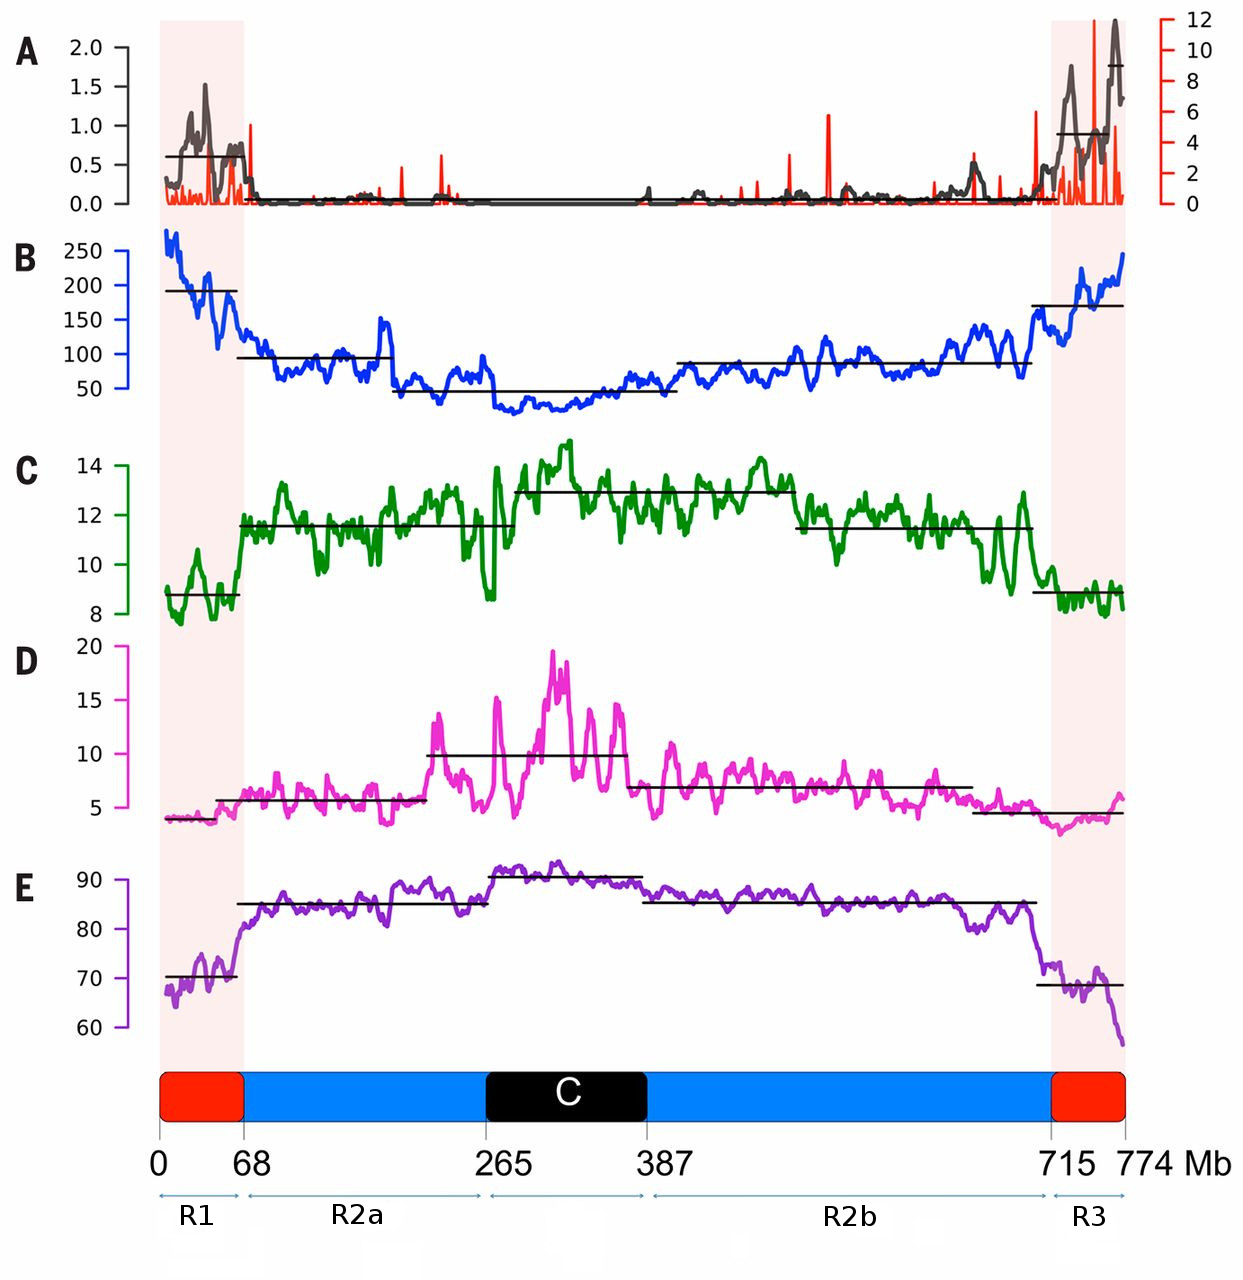
\includegraphics[scale=1.3]{Figures/Figure_1.jpg}
      \vspace{0.5cm}
      \caption{Structural partitioning of the bread wheat chromosome 3B}
      \label{fig:F1}
    \footnotesize{Distribution and segmentation analysis of (A) meiotic recombination rate (cM/Mb in sliding window of 10 Mb in black and 1 Mb in red); (B) gene density, in CDS/10 Mb; (C) expression breadth; (D) average number of alternative spliced transcripts per expressed gene; (E) TE content along the 3B pseudomolecule. 
    
    Distal regions of the chromosome R1 and R3 are represented in red; the centromeric/pericentromeric region (C) is in black and the two internal regions (R2a/R2b) are in blue. The borders of these regions are indicated in Mb. 
    
    Sliding window size: 10 Mb; step: 1 Mb.
    
          \begin{flushright}
          From Choulet \textit{et al.}, \textit{Science}, 2014
          \end{flushright}}
    \end{figure}
\addtocounter{page}{-1}
\newpage
\clearpage % - - - - - - - - - - - % % % FIGURE % % % - - - - - - - - - - - %


            \subsubsection{Sorted chromosome shotgun sequences}

An alternative to the whole genome approach resides in the use of flow cytometry to isolate individual chromosomes or chromosome arms. The development of the flow sorting chromosomes technical allowed scientists to separate the different 42 chromosomes' arms with the aim to sequence each separately in parallel \citep{Dolezel2014}. In 2014, the IWGSC produced a chromosome-based draft sequence of the hexaploid bread wheat though Illumina sequencing. This sequence contains 124,201 gene loci distributed nearly evenly across the homologous chromosomes and subgenomes \citep{Mayer2014}.

However, it's worth noting that neither the whole genome nor the sorted chromosome shotgun approaches can produce a high quality reference sequence as Feuillet \textit{et al.} have defined it \citep{Feuillet2011}. Indeed, the incompleteness of the sequence, its highly fragmented nature and the limited information in terms of locus position relative to each other hamper large scale analysis of the wheat genome organization and its relationship to function and evolution.

            \subsubsection{Physical-map based sequences}

Sorted chromosomes can also be used to construct physical maps and subsequently sequence wheat chromosomes through a so-called \textit{hierarchical shotgun sequencing} approach. This approach relies on the sequencing of individual bacterial artificial chromosome (BAC) clones covering the genome with reduced redundancy.

A pilot project aiming at demonstrating the feasibility of this approach was initiated in 2004. A first BAC library of wheat 3B chromosome was constructed \citep{Safar2004} and used to construct a physical map of this chromosome \citep{Paux2008}, which was improved three years later \citep{Rustenholz2011}. This map served as a template to produce the first reference of a wheat chromosome. It was made through an hybrid approach combining Roche GSFLX sequencing of BAC pools, whole chromosome shotgun by Illumina sequencing as well as Sanger BAC-end sequencing. Scaffolds were anchored and ordered by genetic and linkage disequilibrium (LD) mapping with $\approx$ 3,000 SNPs. Eventually, a 3B pseudomolecule covering 774 Mb was produced \citep{Choulet2k14}.

        \subsection{A giant leap: the chromosome 3B}
            
Access to the chromosome 3B pseudomolecule offered an unprecedented opportunity to analyze the wheat genome to a level that has never been reached before. By combining various approaches including genetic/LD mapping and RNAseq data covering the whole plant development, this sequence was structurally and functionally annotated (Figure \ref{fig:F1}).

\newpage % - - - - - - - - - - - % % % FIGURE % % % - - - - - - - - - - - %
\thispagestyle{empty}
    \begin{figure}
      \centering 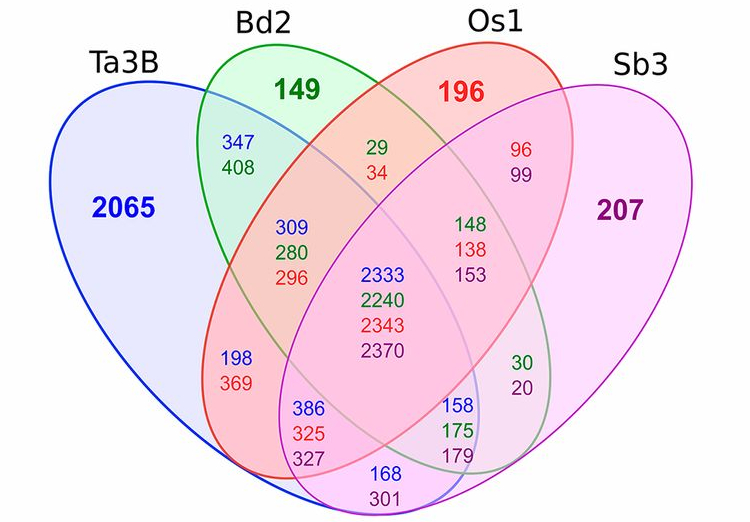
\includegraphics[scale=0.6]{Figures/Figure_2.jpg}
      \vspace{0.5cm}
      \caption{Venn diagram of unique and shared genes between 4 orthologs} 
      \label{fig:F2}
    \footnotesize{Number of conserved genes between wheat 3B chromosome (\textit{Ta3B}), and orthologous chromosomes in rice (Os1), \textit{Brachypodium} (Bd2) and Sorghum (Sb3). 
    
    Numbers shared by two or more species correspond to the number of syntenic genes. Those specific to one species are non-syntenic. An amount of gene is shared when some are specific to one or two species. Wheat seems to be close to \textit{Brachypodium} with 347 shared genes (only 168 with \textit{Shorgo}). A lot of genes (2,065) seem to be wheat-specific, which is $\approx$ 10-fold more than others.
    
          \begin{flushright}
          From Choulet \textit{et al.}, \textit{Science}, 2014
          \end{flushright}}
    \end{figure}
\addtocounter{page}{-1}
\newpage
\clearpage % - - - - - - - - - - - % % % FIGURE % % % - - - - - - - - - - - %


By studying the recombination rate along the chromosome 3B, crossing-overs (COs) were found not to be evenly distributed along the chromosome. Two distal regions, of 68 and 59 Mb on the short and long arms respectively, are showing recombination rates of 0.60 and 0.96 cM/Mb on average. A large proximal region of 648 Mb spanning the centromere with an average recombination rate of 0.05 cM/Mb.

An important fraction of this pseudomolecule was composed of TEs (85\%). 53,288 complete and 181,058 truncated copies of TE, belonging to 485 different families, were annotated by the pipeline CLARI-TE \citep{Daron2014}. The TE density distribution was not random, with a lower density in the distal regions (73\% and 68\%, respectively) compared to the proximal one (88\%). The 122-Mb pericentromeric region displayed the highest density (93\%) of TEs. The speed of elimination of these TEs was also studied, showing a burst of degradation 1 to 3 millions of years after their insertion in the 3B chromosome, especially in the distal regions.

Gene modelling led to predict 7,264 coding loci along the pseudomolecule, whose 5,326 with a functional structure and 1,938 assimilated to pseudogene. RNA-seq analysis conducted in parallel, revealed that 71\% of genes were expressed in at least one condition. Moreover, 3,692 novel transcribed loci were found, that might correspond to long intergenic non-coding RNA or news proteins \citep{Choulet2k14}. A gene density gradient was observed with an increase on both arms along the centromere-telomere axis, correlating with the distance to the centromere.

To assess which genes were conserved during the evolution (syntenic gene), 3B genes chromosome were compared to \textit{B. distachyon}, its closest relative, \textit{O. sativa} ans \textit{Sorghum}. The finding that 94\% of the conserved genes are also present on the 3B sequence suggests that no major gene loss has occurred in the B subgenome yet. In contrast, 2,065 genes on chromosome 3B (34.6\%, including pseudogenes) shared similarity with genes on nonorthologous chromosomes in the other grass genomes. This proportion of nonsyntenic genes is much higher than the 5\% (between 149 and 207) of nonsyntenic genes found in the other analyzed grass species (Figure \ref{fig:F2}). 

In addition, clear relationships between gene position, structure, evolutionary history and expression were observed \citep{Pingault2015}. By combining all these results, a strong structural and functional partitioning of the chromosome 3B was observed, with two distal regions of $\approx$ 60-70 Mb showing an accelerated evolution compared to the large proximal region. These distal regions were actually those with the highest percentage of nonsyntenic, condition-specific and adaptation-related genes. Whether this particular pattern is limited to \textit{Chinese Spring}, to bread wheat or to the whole \textit{Triticum} gender is not clearly defined.

\newpage % - - - - - - - - - - - % % % FIGURE % % % - - - - - - - - - - - %
\thispagestyle{empty}
~
\addtocounter{page}{-1}
\newpage
\clearpage % - - - - - - - - - - - % % % FIGURE % % % - - - - - - - - - - - %


    \section{Plant genomes: all for one or one for all ?}

        \subsection{Evolutionary dynamic and the genome concept}
        
Even if plants are approximately 200-fold older than \textit{Homo}'s gender, if the earth was formed one minute after midnight, plants would have appeared forty-five minutes before the end of the day. However, they spent this time improving their adaptive abilities. By looking around ourselves, it's quite easy to imagine how the plant world could be powerful. He's not only able to survive in a huge range of conditions, but even to evolve thought different offsprings.

While the genome of a given specie has long been considered as stable, the analysis of variations in plants has revealed that their genomes are characterised by high levels of structural variation. The term \textit{structural variations} (SVs) refers to rearrangements such as deletions, duplications, inversions or translocations that impact genome structure and give rise to intraspecific differences. Such variations can affect transposable elements and genes, the latter being often referred to as copy number variations (CNVs) or presence-absence variations (PAVs).

The observations of such SVs between individuals of the same specie indicate that a single genome sequence might not reflect the entire genomic complement of this species, and led to revise the genome concept accordingly. The core genome contains genomic features common to all individuals, while the dispensable genome is composed of partially shared and/or non-shared DNA sequence elements. In addition, some genes called \textit{unique genes} are specific to a single individual. The pangenome describes the full complement of genomic features for a given species and includes the core genome, the dispensable genome as well as unique genes.

While most of these SVs are very likely to be neutral, some can play a role in the adaptation of an individual or a population through the expression of given phenotypes.

        \subsection{Structural variations}
        
            \subsubsection{Types of structural variations}

                \paragraph{Microscopic SVs}
                
Structural variations have been first discovered in the late 1970's. During the 20Th century, most of the variations observed in plants genomes corresponded to changes in chromosome number, size and structure of chromosomes, visible under a microscope. During the past 3 decades, molecular genetic markers have been mostly used in this landscape \citep{Varshney2012}.

\newpage % - - - - - - - - - - - % % % FIGURE % % % - - - - - - - - - - - %
\thispagestyle{empty}
    \begin{figure}
      \centering 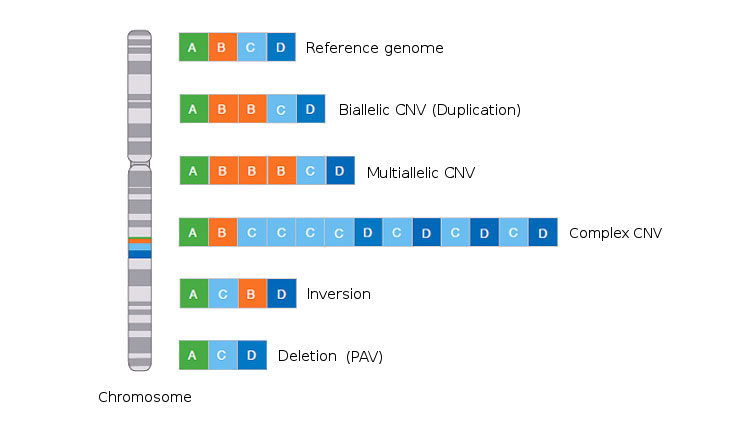
\includegraphics[scale=3]{Figures/Figure_3.jpg}
      \vspace{0.5cm}
      \caption{Different types of structural variations} 
      \label{fig:F3}
\footnotesize{Traditionally, structural variation refers to genomic alterations that are larger than 1 kb in length, but advances in discovery techniques have led to the detection of smaller events. The schematic depicts deletions, mobile-element insertions, tandem and interspersed segmental duplications, inversions and translocations in a test genome (upper line).
    
          \begin{flushright}
          From Feuk \textit{et al.}, \textit{Nat. Rev. Genet}, 2006.
          \end{flushright}}
    \end{figure}
\addtocounter{page}{-1}
\newpage
\clearpage % - - - - - - - - - - - % % % FIGURE % % % - - - - - - - - - - - %


                \paragraph{Submicroscopic SVs}
                
The advent of NGS technologies has offered the opportunity to study SVs at a higher resolution than the microscopic studies described above. Thus, Feuk \textit{et al.} have defined a submicroscopic variant (SV) as a \textit{genomic variations that involve segments of DNA larger than 1 kb in length} \citep{Feuk2006}. Two mechanisms can generate SVs: 
\begin{itemize}
\item[-] Nonhomologous end-joining is the result of an aberrant repair of double-strand break and require low-level of similarity at the breaking points \citep{Iyama2013}
\item[-] Non-allelic homologous recombination requires high-level of similarity to happen \citep{Hurles2006}
\end{itemize}

These mechanisms are able to form different SVs, classified in 3 main groups (Figure \ref{fig:F3}).

            \subparagraph{Copy number variations (CNV)}
            
The term CNV refers to loci that demonstrate a variable copy number between individuals. This polymorphism is due to duplication events, sometimes followed by deletions of a small portions of the duplicated segments \citep{Redon2006}. It can concern DNA sequences from 1 kb to several Mb, and CNVs are prevalent in most of plant genomes \citep{Zmienko2013}.

            \subparagraph{Presence/absence variations (PAV)}
                    
PAVs can be seen as an extreme case of CNVs. it defines sequences that are present in some individuals but absent from others. Deletions or insertions can create PAV in a genome, causing lacks or gains of sequences. It can affect both non-coding sequences (like TEs) or genes.

            \subparagraph{Inversions, translocations}

Beside CNVs and PAVs, inversions or translocations of genomic fragments can arise in genome. Such SVs can affect large fragments such as chromosome arms or small regions and can be the driver of speciation. This kind of variations have been charracterized in nuclear genome, leading to infertility \citep{Mach2011} or playing a role in the plant adaptation \citep{Kirkpatrick2010}, thus showing negative or beneficial potential of these SV. In addition, some of these variations were detected even in mitochondrial \citep{Mackenzie1999} or in chloroplast genome \citep{Kim2005}.
    
            \subsubsection{Detection techniques}
            
                    \paragraph{Microarray-based approaches}

Two types of microarray-based technicals are used for SVs detection. First, the comparative genomic hybridization array (aCGH) was developed since 1997 \citep{Solinas-Toldo1997}. 

\newpage % - - - - - - - - - - - % % % FIGURE % % % - - - - - - - - - - - %
\thispagestyle{empty}
~
\addtocounter{page}{-1}
\newpage
\clearpage % - - - - - - - - - - - % % % FIGURE % % % - - - - - - - - - - - %

The reference sequence is registered on a microarray and the compared genome is hybridized above, allowing to detect differences thanks to different fluorophores used as probes. The second one, SNP array, is also based on hybridization, but the DNA probes are specifically designed to detect really small differences. Thus, the sensitivity is significantly increased and  distinguishing alleles became more easy.

                    \paragraph{Sequencing / resequencing approaches}

The development of NGS technologies allowed scientist to use them for SVs detection. Several technicals are possible, but are all based on mapping strategy. Reads of sequencing from the studied organism are mapped on a reference genome to detect variations. All of the variations are detectable with this technical, which become more and more cheaper.

        \subsection{Structural variations in plants}

With the advent of NGS, the number of publications dealing with CNVs in plant genomes has increased exponentially over the past years. In human health, it's now admitted that CNV are responsible for number of diseases : psoriasis \citep{Hollox2008}, osteoporosis \citep{Yang2008}, HIV susceptibility \citep{Gonzalez2005} or many cancers \citep{Stadler2012}. But plant world wasn't stripped away with 402 \textit{Arabidopsis Thaliana}'s genes described as variants \citep{DeBolt2010}, and recently 4 genes were used for CNV analysis between 16 potato cultivars \citep{Iovene2013}.

Maize inbred line B73 was the first specie highly-genotyped for CNV detection \citep{Springer2009}. CGH analysis on maize were focused on coding regions from several lines and detected that CNV were found on most of maize chromosome, but at a lower rate near the centromer \citep{Belo2010}.

More recently, 641 CNV were identified by CGH, distinguishing two rice cultivars who have diverged 0.4 million years ago (\textit{O. sativa japonica} and \textit{O. sativa indica}). These variations were found all along the 12 chromosomes, representing 1.8\% of the total genome and are in majority shorter than 10kb \citep{Yu2011}. Lately, this analyse was performed again with 20 Asian cultivars, increasing the number of gene overlapped by a CNV at 1,321 \citep{Yu2013}.

In soybean, three cultivars were analysed for CNV array-based detection. Hundreds of variations were so detected, with a median-size of 20 kb and a heterogeneous distribution \citep{McHale2012}. In 2014, two DNA sequences from Asian cultivars were studied, revealing 4,000 stop codons present in a variety, but not in the other one \citep{Li2014}.

Cereals were thus quite studied last years. But, due to the agronomical context, \textit{Triticeaes} are since 5 years the most genomic-studied group in plant kingdom.

\newpage % - - - - - - - - - - - % % % FIGURE % % % - - - - - - - - - - - %
\thispagestyle{empty}
~
\addtocounter{page}{-1}
\newpage
\clearpage % - - - - - - - - - - - % % % FIGURE % % % - - - - - - - - - - - %


        \subsection{What about \textit{Triticeae} ?}
        
Barley was one of the first \textit{Triticeae} to be studied for CNV \citep{Munoz-Amatriain2013}. Fourteen different genotypes were used for CGH, indicating a variation in 14.9\% of the gene set, mainly located in distal regions. GO-term enrichment analysis revealed that genes affected are belonging to categories \textit{cell death} and \textit{protein modification}, genes often implicated in disease resistance.

In wheat, the use of CGH arrays is hampered by the presence of homeologous copies that prevent the efficient detection of SVs. However, in 2011, a study have permitted, thanks to NGS, to affirm that gene duplications are prevalent in cultivated wheats, while deletions occurred in wild wheats \citep{Saintenac2011}. But this analyse was focused on only 3,497 cDNA, representing 3.5 Mb of the 17 Gb in total.

One year after, it was proved that the capacity of early flowering in several wheats is coming from a CNV. A duplication of the \textit{Ppd-B1} gene, implied in measure of photoperiod, cause an early flowering, while a duplication of \textit{Vrn-A1}, implied in vernalization process, cause a late-flowering \citep{Diaz2012}. The same year, it was showed that the dwarf gene \textit{Rht-D1} can be under CNV pressure. Thus, two copies of Rht-D1b were three-fold more effective in reducing plant height than a single copy \citep{Li2012}.

However, no genome-wide studies has been performed in wheat and the lack of reference has long made impossible to investigate SVs in regard to the genome organization.

    \section{Internship's subject}

        \subsection{Resequencing of 45 varieties}
        
In addition to the reference cultivar \textit{Chinese Spring}, forty-four 3B chromosomes were sequenced with a depth ranging between 13 and 57x (Appendix 1). This panel was selected to maximize geographic, ploidy and genetic diversity. Indeed, 7 tetra or hexaploid species are represented: \textit{T. carthlicum, T. diccocoides, T. dicoccum, T. durum, T. spelta, T. macha} and \textit{T. aestivum}.

Thus, this sampling covers all continents and different phenotypical traits of interest. For example, a variety can have a high tillage (\textit{Triticum durum desf.}, Svevo), while another can be cold-resistant (\textit{Triticum aestivum aestivum}, Marquis).

        \subsection{From CGH to NGS}

As shown before, most of the CNV studies conducted in the past years used CGH array-based technology. However, microarray do have several intrinsic limitations. 

\newpage % - - - - - - - - - - - % % % FIGURE % % % - - - - - - - - - - - %
\thispagestyle{empty}
~
\addtocounter{page}{-1}
\newpage
\clearpage % - - - - - - - - - - - % % % FIGURE % % % - - - - - - - - - - - %

First, it is quite hard and expensive to design microarray for an unknown or incomplete reference genome. Then, the noise, detected with these array, limits the range of high-confidence data, making the detection of low-abundance sequences difficult. Finally, some limits were observed concerning the reproducibility of microarray data \citep{Ioannidis2009}.

Whole genome sequencing is now widely used to characterize genetic variations \citep{Rubin2010}. Thus, the use of NGS data for CNV detection allows to avoid obstacles brought by CGH. Indeed, assembled reference genome isn't required, quantification of signal from sequence-based approaches is accurate. Finally it is more cost-efficient and requires less input DNA than an array \citep{Hurd2009}.

        \subsection{Transpositional, then transcriptional}

By studying transpositional landscape (TE presence or absence on 3B chromosome between those 45 varieties) among the \textit{Triticeae} last year, the intraspecific diversity was described as quite variable in this group. Indeed, an average of 15\% of the ISBP markers are different between a variety and the reference \textit{Chinese Spring}. Differences ranged from 7\% to 45\% between \textit{Chinese Spring} and the forty-four others 3B chromosome. These variations can certainly explain part of the diversity observable between different wheat accessions (like diseases resistance, grow time, nitrogen need ...) but not only. 

Even if the non-coding regions are the main constituents of the 3B chromosome, completing this intraspecific diversity analysis through CNV in genic portion is essential. Genes are often carried by TEs during their moves along the DNA, so the results from these two analysis will be easy to correlate.

        \subsection{Objectives}

This work aimed at studying the diversity in the coding fraction of the 3B chromosome of forty-four resequenced wheat accessions compared to the reference sequence of \textit{Chinese Spring}'s 3B chromosome. The CNV occurring in genic segments were identified for each variety, leading to large polymorphism detection among homogeneous wheat population.

\newpage % - - - - - - - - - - - % % % FIGURE % % % - - - - - - - - - - - %
\thispagestyle{empty}
~
\addtocounter{page}{-1}
\newpage
\clearpage % - - - - - - - - - - - % % % FIGURE % % % - - - - - - - - - - - %


% ----------------------------------------
% ----------------------------------------
% MAT&MET
% ----------------------------------------
% ----------------------------------------
\part{Material and methods}
\setcounter{section}{0}

    \section{Biological material and DNA sequences}
    
Forty-four \textit{Triticum} accessions were selected for this analysis from the Biological Resource Center (CRB) of the INRA GDEC research unit (Appendix 1). A maximum diversity is represented in this panel, involving differences at several levels. This set includes twenty \textit{Triticum aestivum}, three \textit{T. spelta}, three \textit{T. macha}, seven \textit{T. durum}, four \textit{T. dicoccum}, four \textit{T. carthlicum} and three \textit{T. dicoccoides}. They are also coming from a large part of the land cultivating cereals (19 countries).

Chromosome 3B was isolated from these 44 accessions through flow cytometry \citep{Dolezel2014}. Following whole-genome amplification, sorted chromosomes were sequenced on an Illumina HiSeq2000, with 2 x 100-bp paired reads. Sequencing depth ranged from 13X (\textit{Arche}) to 57x (\textit{33800}). 

    \section{Read mapping process}
    
Sequencing reads were mapped to the chromosome 3B reference sequence \citep{Choulet2k14} using BWA-mem 0.7.10 algorithm \citep{LiBWA2009}. Mapping data were then processed using Samtools 1.1 \citep{LiSAMTOOLS2009} and Bedtools 2.18.2 \citep{Quinlan2010}. Theses informatic tools allow to manipulate files from the mapping process (extracting coverage data, select trimmed reads ...). 

All analyses were performed on the high-performance cluster \textit{Saruman}, (864 threads) located at URGI, Versailles, France. A bioinformatic pipeline incorporating all the different steps has been developed for automated analysis (Appendix 2).

    \section{Normalization and statistics}
    
Alignments were finally visualized using Integrate Genome Browser \citep{Thorvaldsdottir2013}. The number of reads mapped to each genic feature was extracted using Bedtools Coverage script. A five-step normalization process was then applied to raw mapping data. 

\newpage % - - - - - - - - - - - % % % FIGURE % % % - - - - - - - - - - - %
\thispagestyle{empty}
~
\addtocounter{page}{-1}
\newpage
\clearpage % - - - - - - - - - - - % % % FIGURE % % % - - - - - - - - - - - %

\vspace{0.5cm}
(1) \hspace{2cm} $R_{1} = R \cdot \frac{\bar{x}}{X_{GC\%}}$
\vspace{0.5cm}

With R being the average read count mapped in a given feature, $\bar{x}$ the average coverage of all features for a given accession and $X_{GC\%}$ the average coverage of genes having similar GC content (from 29, 30, 31 ... to 80\%). This normalization allows getting rid  of the mapping bias caused by GC content differences between regions. 

\vspace{0.5cm}
(2) \hspace{2cm} $R_{2} = \frac{R_{1} \cdot S_{genes}}{R_{genes} \cdot S_{read}}$
\vspace{0.5cm}

With $R_{1}$ being the result of the previous normalization step (1), $S_{genes}$ the cumulative feature length (19.82 Mb) along \textit{Chinese} 3B chromosome, $R_{genes}$ the total number of reads mapped in genic features for a given accession, and $S_{read}$ the read length (100 bp). This steps normalize differences in sequencing depth for all accessions.

\vspace{0.5cm}
(3) \hspace{2cm} $R_{3} = \frac{R_{2}}{\frac{\%C_{Accession}}{\%C_{ChineseSpring}}}$
\vspace{0.5cm}

With $R_{2}$ being the result of the previous normalization step (2), $\%C_{Accession}$ the percentage of the feature covered in a given accession, and $\%C_{ChineseSpring}$ the percentage covered in \textit{Chinese Spring}.

\vspace{0.5cm}
(4) \hspace{2cm} $R_{4} = \frac{R_{3}}{R_{3 Chinese}}$
\vspace{0.5cm}

With $R_{3}$ being the result of equation (3) and $R_{3 Chinese}$ the normalized $R_{3}$ value for \textit{Chinese Spring}. This is the comparison between studied variety and the reference.

\vspace{0.5cm}
(5) \hspace{2cm} $R_{5} = \log_2{R_{4}}$
\vspace{0.5cm}

With this final calculation, \textit{Chinese Spring} have no difference at each locus with himself and every $R_{5}$ value is directly comparable with this reference.

Thus, the different analysis were made on a 45 x 7264 matrix containing all of the corrected means of coverage $R_{5}$ for the 7,264 genes for 45 wheat accessions. Every plots and statistical analysis were then processed with R scripts under Rstudio development tool \citep{Ihaka1996}.

% - - - - - - - - - - - % % % FIGURE % % % - - - - - - - - - - - %
\newpage 
\thispagestyle{empty}
    \begin{figure}
    \vspace{-1.5cm}
      \centering 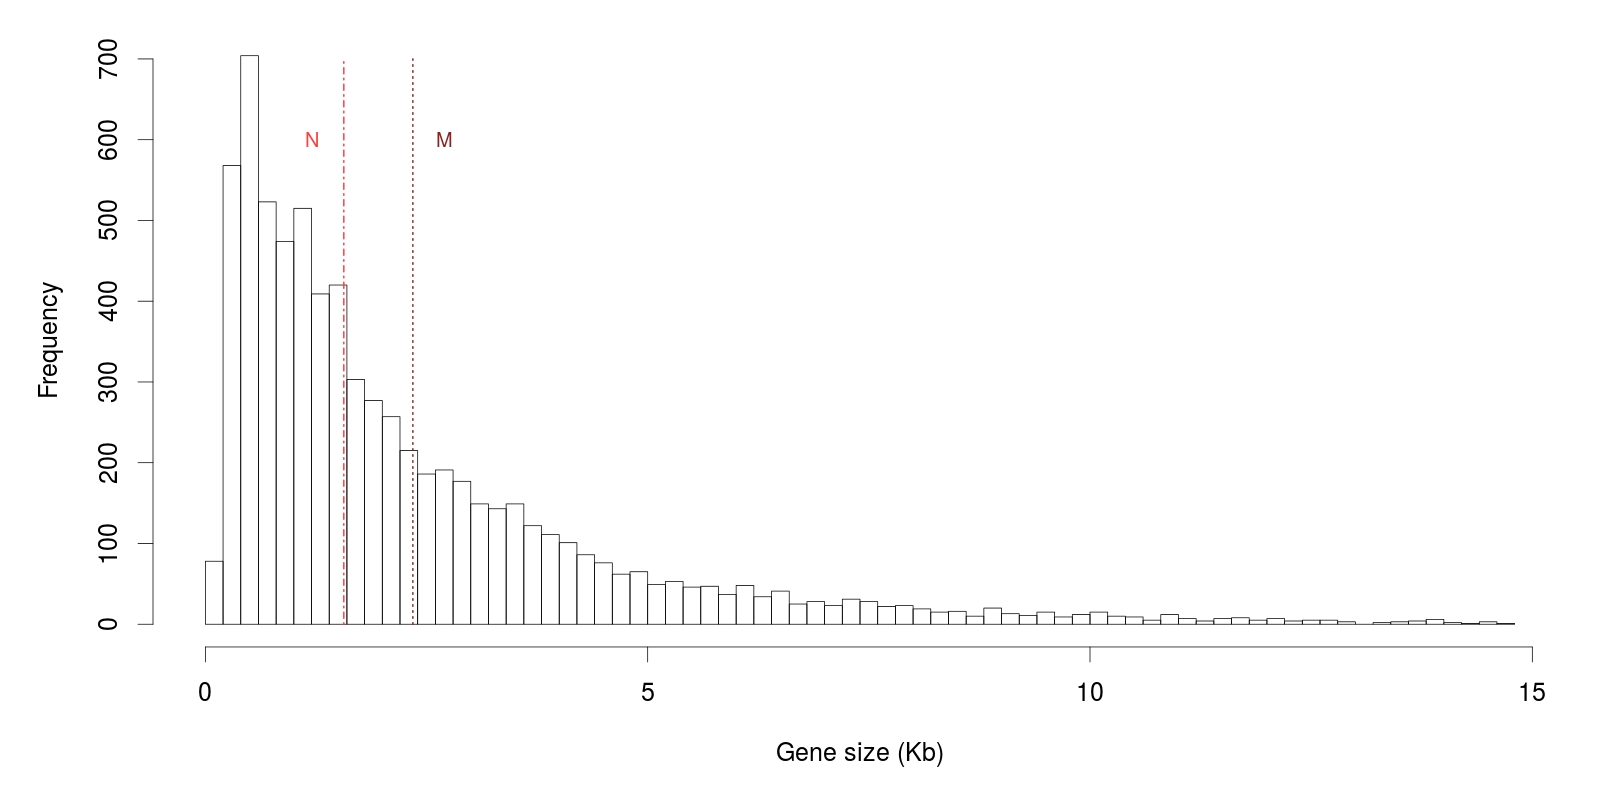
\includegraphics[scale=0.19]{Figures/Figure_4.jpg}
      \vspace{0.5cm}
      \caption{Distribution of the \textit{Chinese Spring} chromosome 3B gene lengths} 
      \label{fig:F4}
\footnotesize{Each bar represents the number of genes in a given size class. A large amount of gene is smaller than 5 kb, but the mean is centred on 2.7 kb (brown dotted line, M). The N50 is at 1.2 kb (red dashed line, N) indicating that 50\% of the genes are smaller than 1.2 kb. The high amount of small genes is due to the presence of pseudogenes along the 3B pseudomolecule.}
    \end{figure}
% - - - - - - - - - - - % % % FIGURE % % % - - - - - - - - - - - %    
    \begin{figure}
    \vspace{-0.7cm}
      \centering 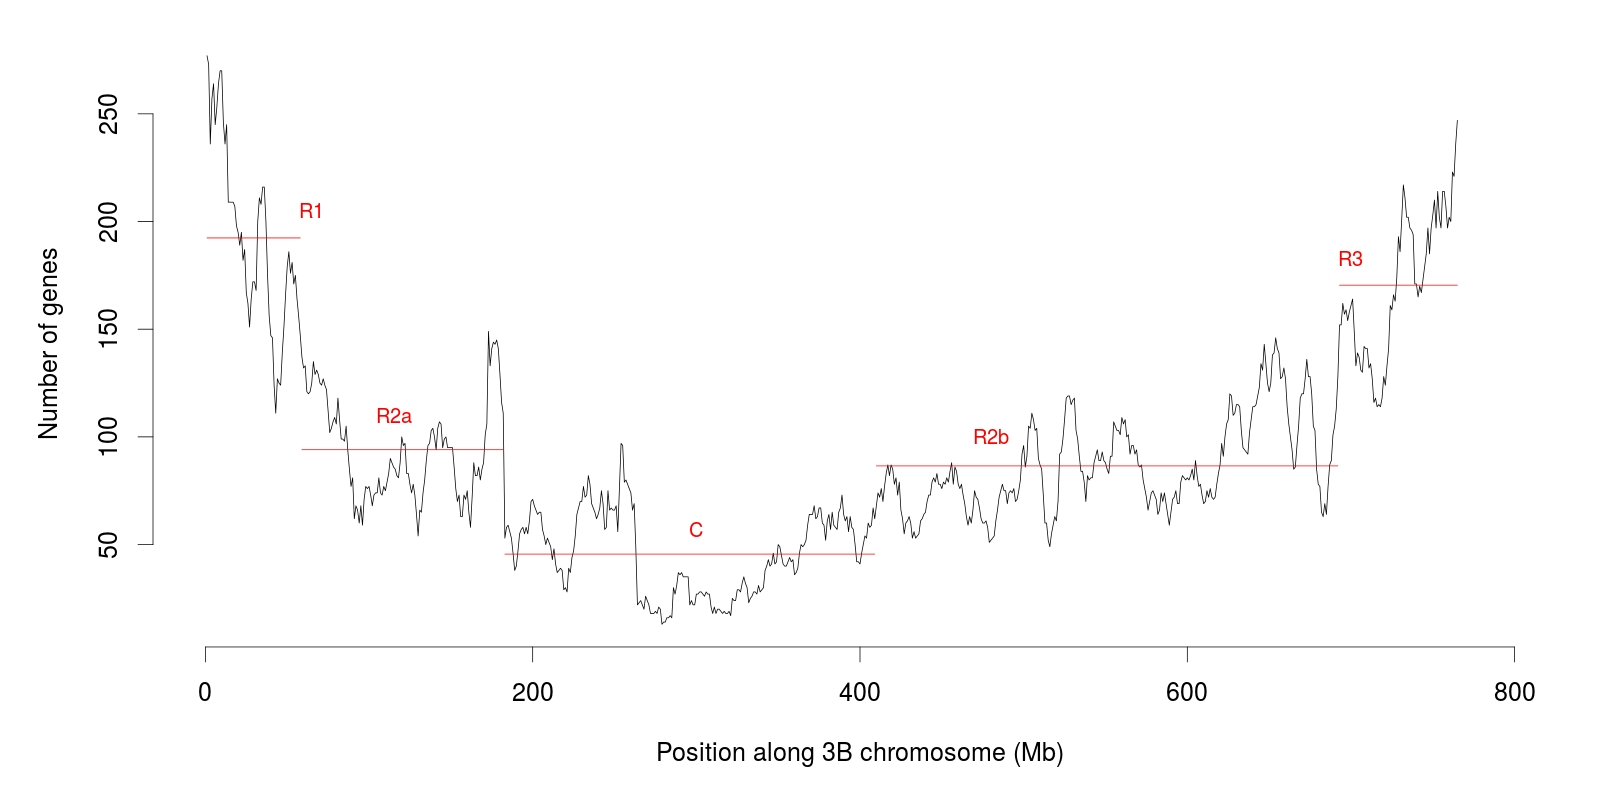
\includegraphics[scale=0.19]{Figures/Figure_5.jpg}
      \vspace{0.5cm}
      \caption{Distribution of the gene density along \textit{Chinese Spring} 3B chromosome} 
      \label{fig:F5}
\footnotesize{This segmentation of the gene number in a 10 Mb windows sliding with a 1 Mb step along 3B shows five regions on the chromosome. Two distal regions R1 and R3, two proximal regions R2a and R2b and a pericentromeric region C. This segmentation is reliable to the one detected by Choulet \textit{et al.} during their analyses. The gene density is higher in the distal regions compared to the pericentromeric one, with $\approx$ 4-fold more genes.}
    \end{figure}
% - - - - - - - - - - - % % % FIGURE % % % - - - - - - - - - - - %
    \begin{figure}
    \vspace{-0.7cm}
      \centering 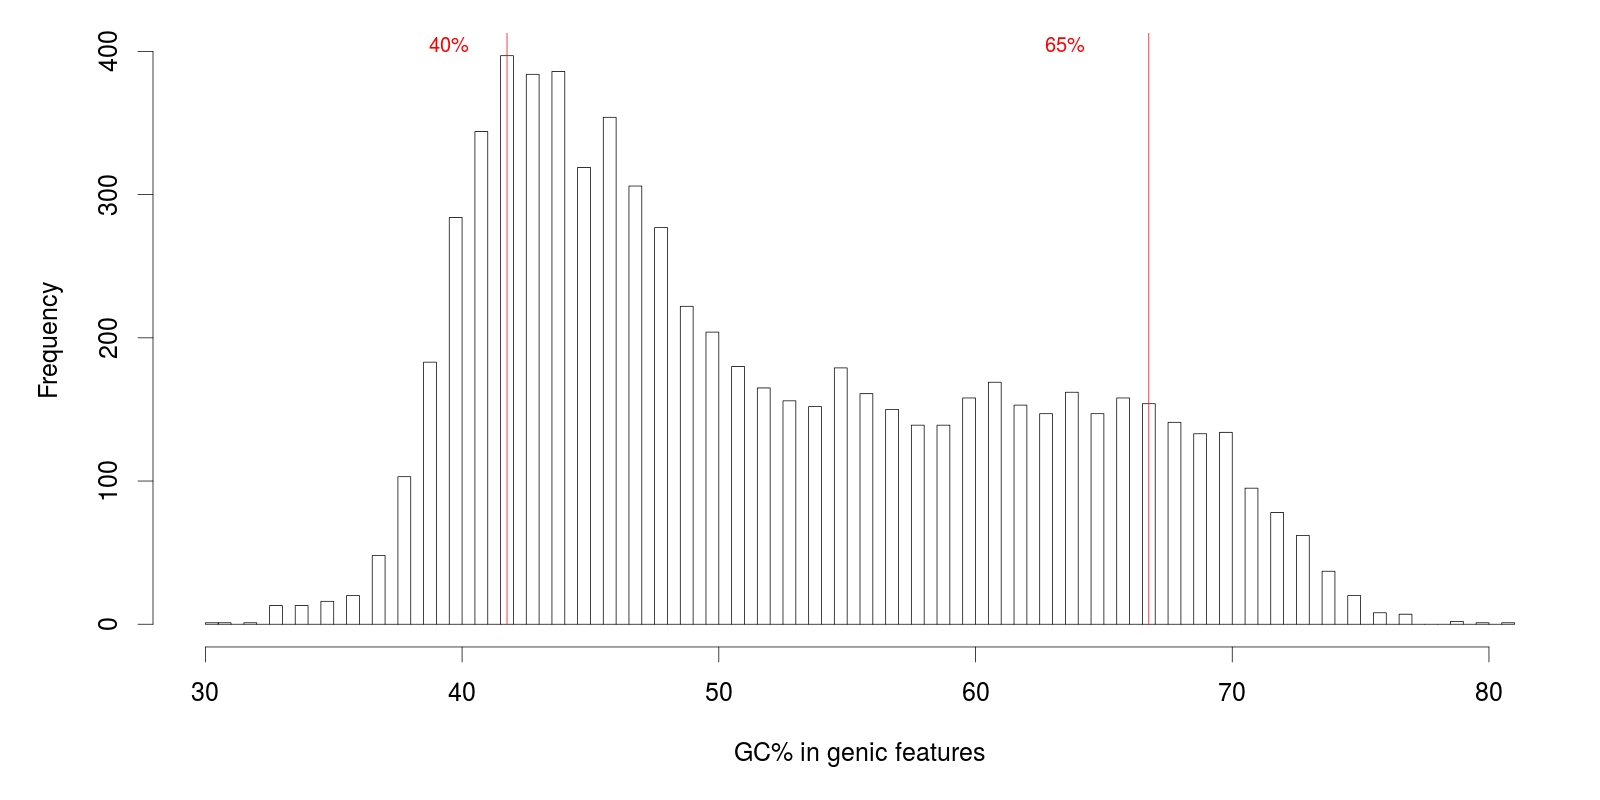
\includegraphics[scale=0.19]{Figures/Figure_6.jpg}
      \vspace{0.5cm}
      \caption{Distribution of GC content in genic regions} 
      \label{fig:F6}
\footnotesize{Each bar represents the number of genes in a given \%GC class. The GC percentage of each gene was calculated with a local Perl script. This representation fit a bimodal distribution centred around 40 and 65\% (red lines).}
    \end{figure}
\addtocounter{page}{-1}
\newpage
\clearpage 
% - - - - - - - - - - - % % % FIGURE % % % - - - - - - - - - - - %

% ----------------------------------------
% ----------------------------------------
% RESULTS
% ----------------------------------------
% ----------------------------------------
\part{Results}
\setcounter{section}{0}

    \section{Genic fraction along \textit{Chinese Spring}'s 3B}

A total number of 7,264 genes were annotated along the \textit{Chinese Spring}'s 3B chromosome reference sequence, with a variable size from 110 bp to 334 kb (Figure \ref{fig:F4}). The gene set, visible on the graph, has an average size of 2.35 kb (brown dotted line, M) and a N50 of 1.57 kb (red dashed line, N), indicating that half of the total number of gene are smaller than this value. Most of genes have a length around 0.5 kb and then, the amount of gene decrease for each size. However, only 71 genes have a length smaller than 0.2 kb (0.97\%). These tiny portions are not complete genes, but pseudogenes, which can be functional or not.

The total number of gene was then estimated in a 10 Mb visualisation window sliding with a 1 Mb step along the 3B chromosome from \textit{Chinese Spring} (Figure \ref{fig:F5}). Genes are not equally distributed, with an average number of 190 genes per 10 Mb-windows in distal regions \textit{vs.} 50 in the proximal one. Segmentation of the plot with \textit{SegNeigh} method allowed to recover the different sections of the 3B chromosome found before by Choulet \textit{et al}. Distal regions, exhibiting the highest numbers of genes are called R1 and R3. Proximal region, annotated C, is around the centromere and is flanked by two intermediary regions (R2a and R2b). By knowing that recombination is more important around telomeres, the distal gene content is largely prone to evolution.

The GC content was also calculated for each genic fraction (Figure \ref{fig:F6}). The amount of GC bases in a genic sequence range from 29.7 to 80.5\%, but the graphic representation fit a bimodal distribution, with the main shoulder centred on 40\%. It fits the expected result, the average GC content in genes is 45\% in monocot plants and 41\% in animals.

    \section{Validation of NGS data}

        \subsection{Depth of sequencing comparison}
        
Each accession was sequenced at different depth of sequencing, involving different coverage at the same nucleotidic position for each variety and representing the theoretical coverage. Following every raw sequences mapping, the number of mapped reads from all accessions gave an observed coverage.

% - - - - - - - - - - - % % % FIGURE % % % - - - - - - - - - - - %
\newpage 
\thispagestyle{empty}
        \begin{figure}
        \vspace{-1.5cm}
          \centering 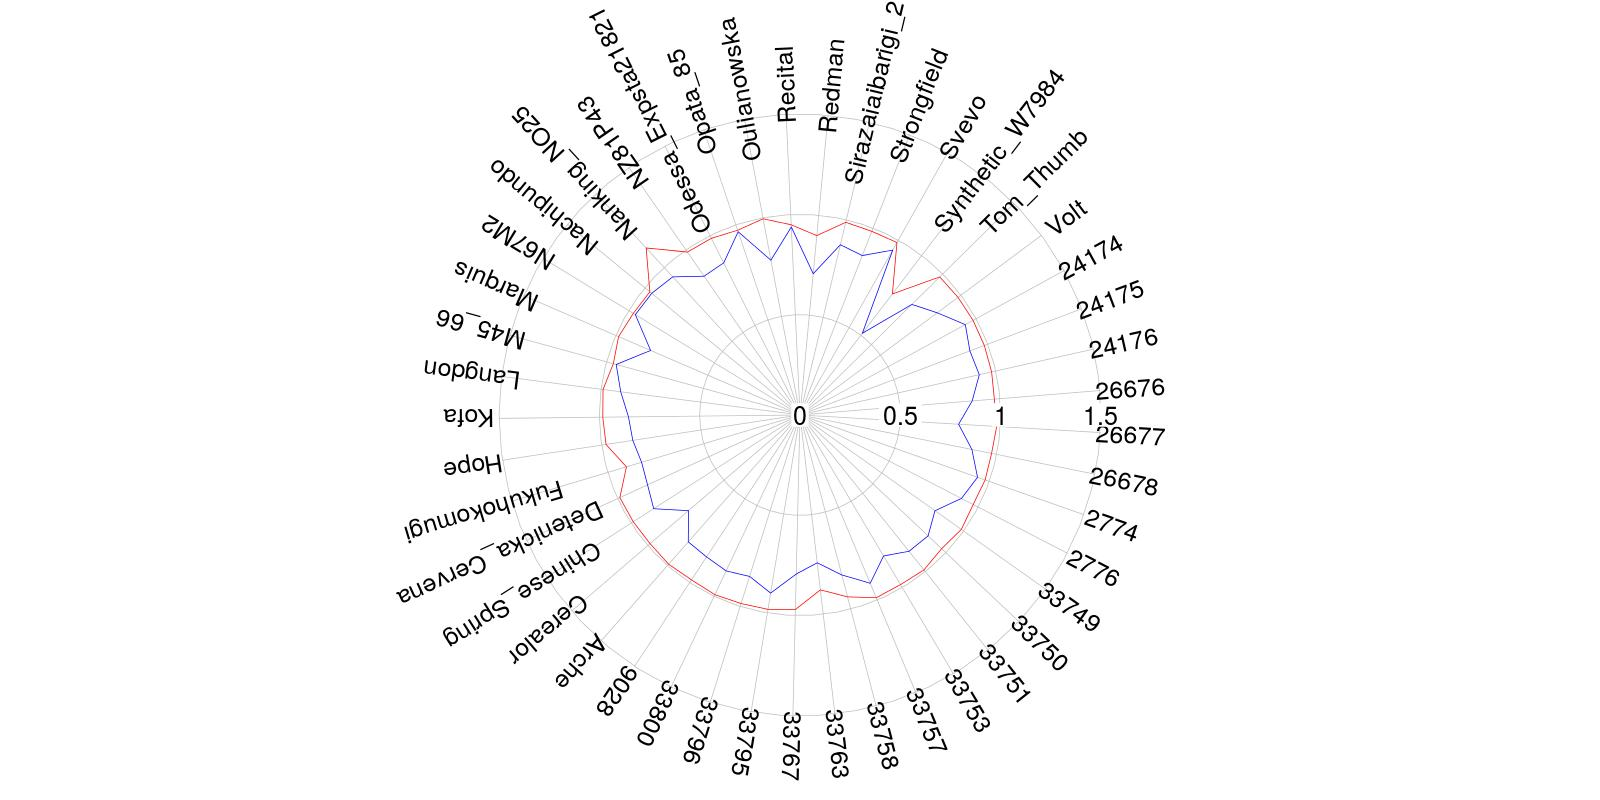
\includegraphics[scale=0.2]{Figures/Figure_7.jpg}
          \vspace{0.5cm}
          \caption{Ratio between expected and observed sequencing depth}
          \label{fig:F7}
        \footnotesize{The expected sequencing depth is calculated with the total number of reads in the sequencing file and the observed one is the mean of the coverage of each nucleotide after mapping, without (red line) and with (blue line) removal of optical duplicate reads created by sequencing. This \textit{red} ratio is close to 1 for every accession (red line), while the \textit{blue} one is slightly lower as a result of a lower number of mapped reads.}
        \end{figure}
% - - - - - - - - - - - % % % FIGURE % % % - - - - - - - - - - - %
        \begin{figure}
        \vspace{-0.7cm}
          \centering 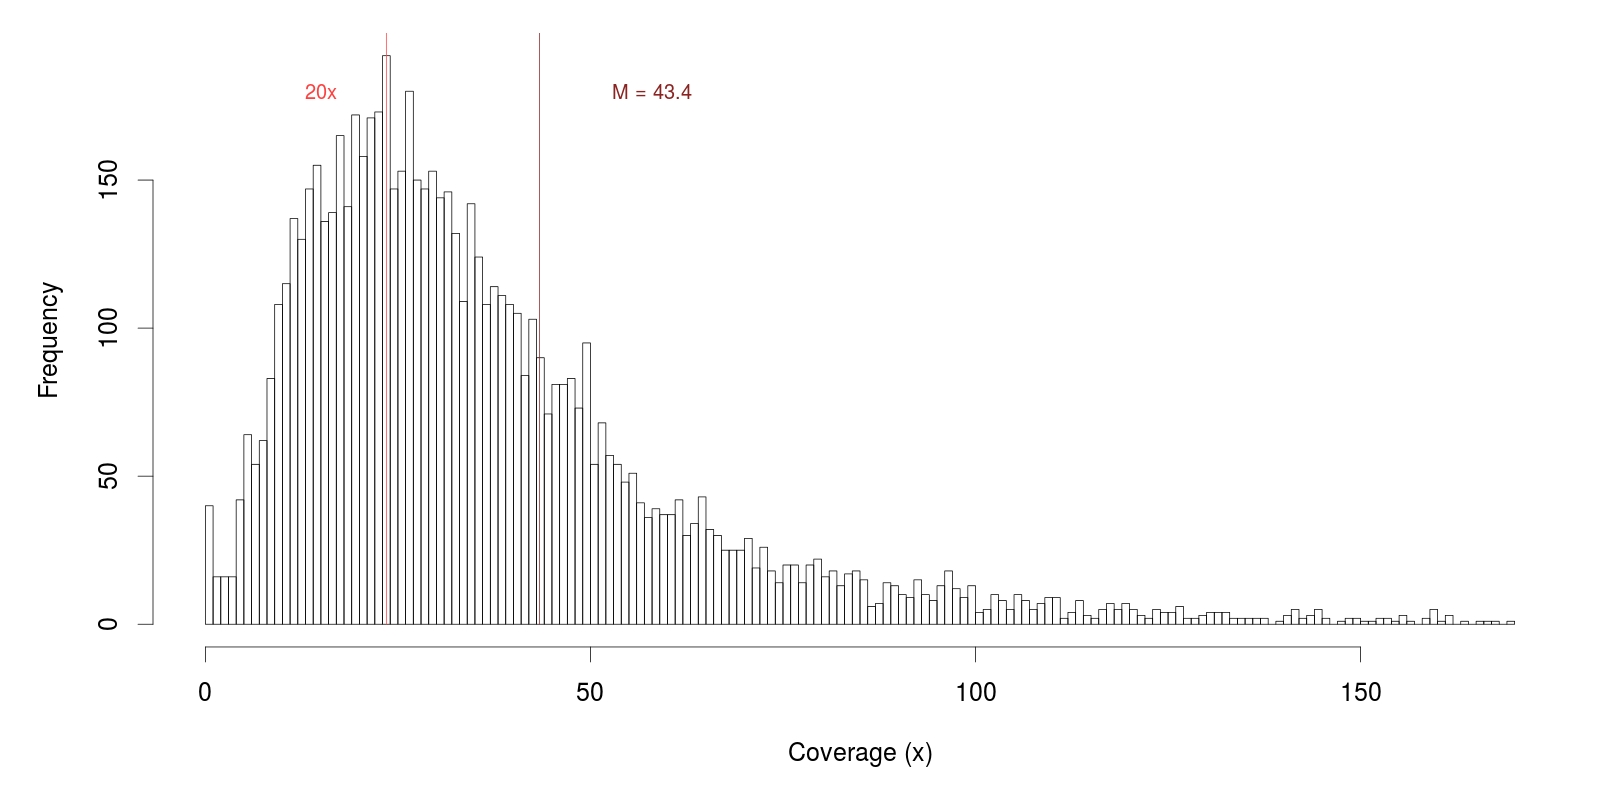
\includegraphics[scale=0.2]{Figures/Figure_8.jpg}
          \vspace{0.5cm}
          \caption{Frequency of gene coverage in the CSvCS mapping} 
          \label{fig:F8}
        \footnotesize{Gene coverage was calculated following mapping of \textit{Chinese Spring} sorted chromosome 3B reads onto the 3B pseudomolecule. Each bar represents the number of genes in a given coverage class. The curve is centred around 20x (red line), but the average coverage is 43.4x (brown line), corresponding to the expected coverage (40X).}
        \end{figure}
% - - - - - - - - - - - % % % FIGURE % % % - - - - - - - - - - - %
        \begin{figure}
        \vspace{-0.7cm}
          \centering 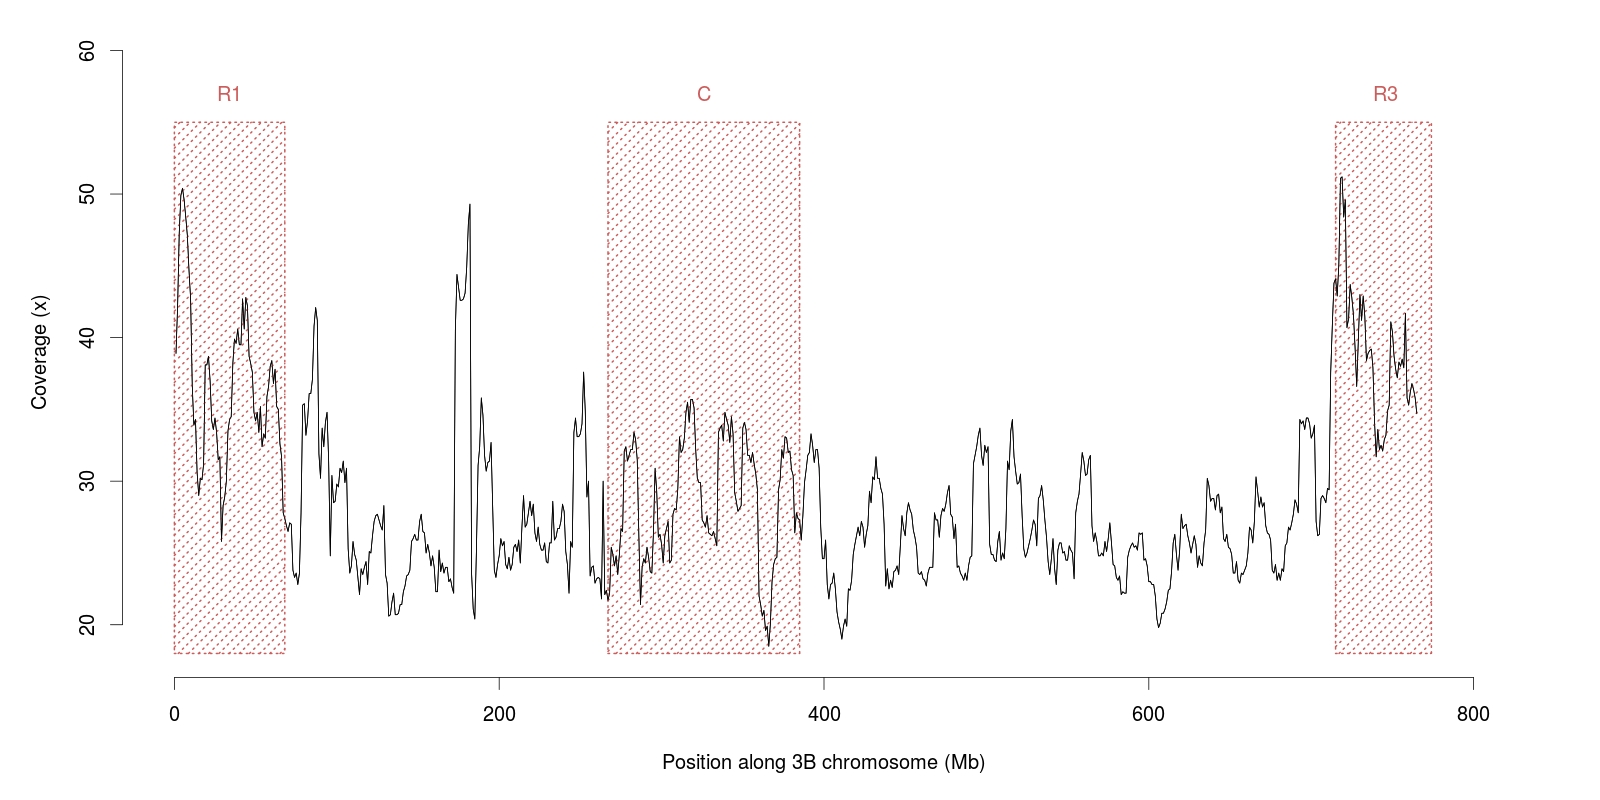
\includegraphics[scale=0.2]{Figures/Figure_9.jpg}
          \vspace{0.5cm}
          \caption{Distribution of gene coverage in the CSvCS mapping} 
          \label{fig:F9}
        \footnotesize{The average gene coverage was calculated in a 10-Mb sliding window. The gene coverage is higher in the distal regions ($\approx$ 40x) than in the centromeric one ($\approx$ 25-30x). The red dashed areas are the chromosomal regions R1, C and R3 defined by Choulet \textit{et al.}.}
        \end{figure}

\addtocounter{page}{-1}
\newpage
\clearpage 
% - - - - - - - - - - - % % % FIGURE % % % - - - - - - - - - - - %

The \textit{theoretical/observed} coverage ratio was thus calculated, and varies from 0.86 for \textit{Nanking No25} to 1.29 for \textit{Tom Thumb} (Figure \ref{fig:F7}, red curve) but is centred on an average ratio of 0.97. The percentage of mapped reads was also calculated, ranging from 88.46\% (\textit{Fukuhokomugi}) to 97.15\% (\textit{Marquis}) of the total number of reads generated by sequencing.
    
        \subsection{\textit{Chinese Spring} \textit{vs.} \textit{Chinese Spring} mapping}
        
Raw NGS data from \textit{Chinese Spring}'s 3B chromosome resequencing were mapped on the reference sequence to validate the method, mapping referred to as \textit{CSvCS}. Considering that sequencing reads and reference sequence are coming from the same variety, every annotated gene along the pseudomolecule should be covered by resequencing reads. An amount of 6,425 genes (88\%) were covered at 100\% by reads. The other 839 genes were covered from 0\% for 2 genes to 99.9994\%. In other terms, the frequency of each depth of coverage was plot (Figure \ref{fig:F8}). Thus, a majority of genes should be covered. The curve reach the peak around 20x with more than 200 genes with this coverage but considering all the genes, the average coverage in these features is 43.4x, as planned by the calculation of the expected coverage.

Average coverage of \textit{Chinese}'s genes by its reads was also plotted along 3B chromosome (Figure \ref{fig:F9}). Obviously, every sections of the 3B chromosome aren't covered equally. Indeed, this mapping exhibit coverages from 20x (mainly in C region) to more than 50x (in R1/R3 regions), indicating regions more amplified during whole genome amplification (WGA), just before sequencing. Some TEs have already been described as absent after a WGA process, thus some regions of the 3B chromosome could have be more amplified (distal parts) when C region could have been less.

A peak can also be observed at position $\approx$ 180 Mb: it is due to mitochondrial DNA inserted in the 3B chromosome, strongly repeated. Thus, all of these values allow the use these data for CNV/PAV detection, thanks to their good quality.

    \section{Mapping. Who's absent ?}
    
        \subsection{Verification of mapping data}

Mapping was so carried by using \textit{BWA-mem} algorithm. First of all, a really strong correlation is visible between the total number of reads and the expected coverage of each accession (Figure \ref{fig:F10}). Every dot is around the red dotted correlation line with a $R^{2}$ = 0.996, indicating that the coverage of mapped reads for each accession is a function of the total number of reads coming from the sequencing.

% - - - - - - - - - - - % % % FIGURE % % % - - - - - - - - - - - %
\newpage 
\thispagestyle{empty}

    \begin{figure}
    \vspace{-1.8cm}
      \centering 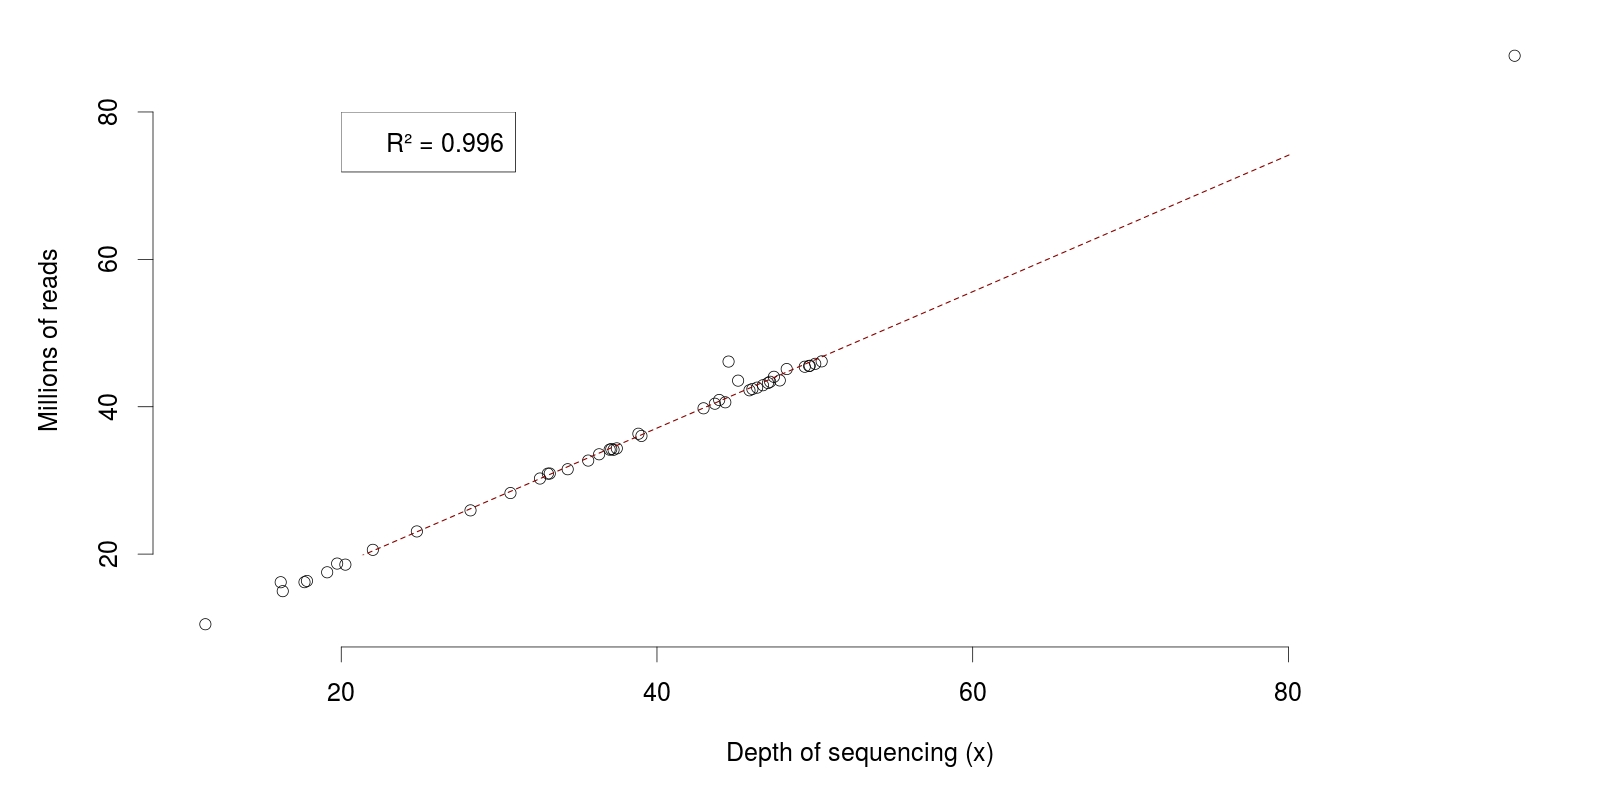
\includegraphics[scale=0.2]{Figures/Figure_10.jpg}
      \vspace{0.5cm}
      \caption{Correlation between the number of mapped read and the expected coverage} 
          \label{fig:F10}
        \footnotesize{Each dot represents an accession. The number of mapped reads is a linear function of the total number of reads for the 45 accessions.}
    \end{figure}
% - - - - - - - - - - - % % % FIGURE % % % - - - - - - - - - - - %
    \begin{figure}
    \vspace{-1cm}
      \centering 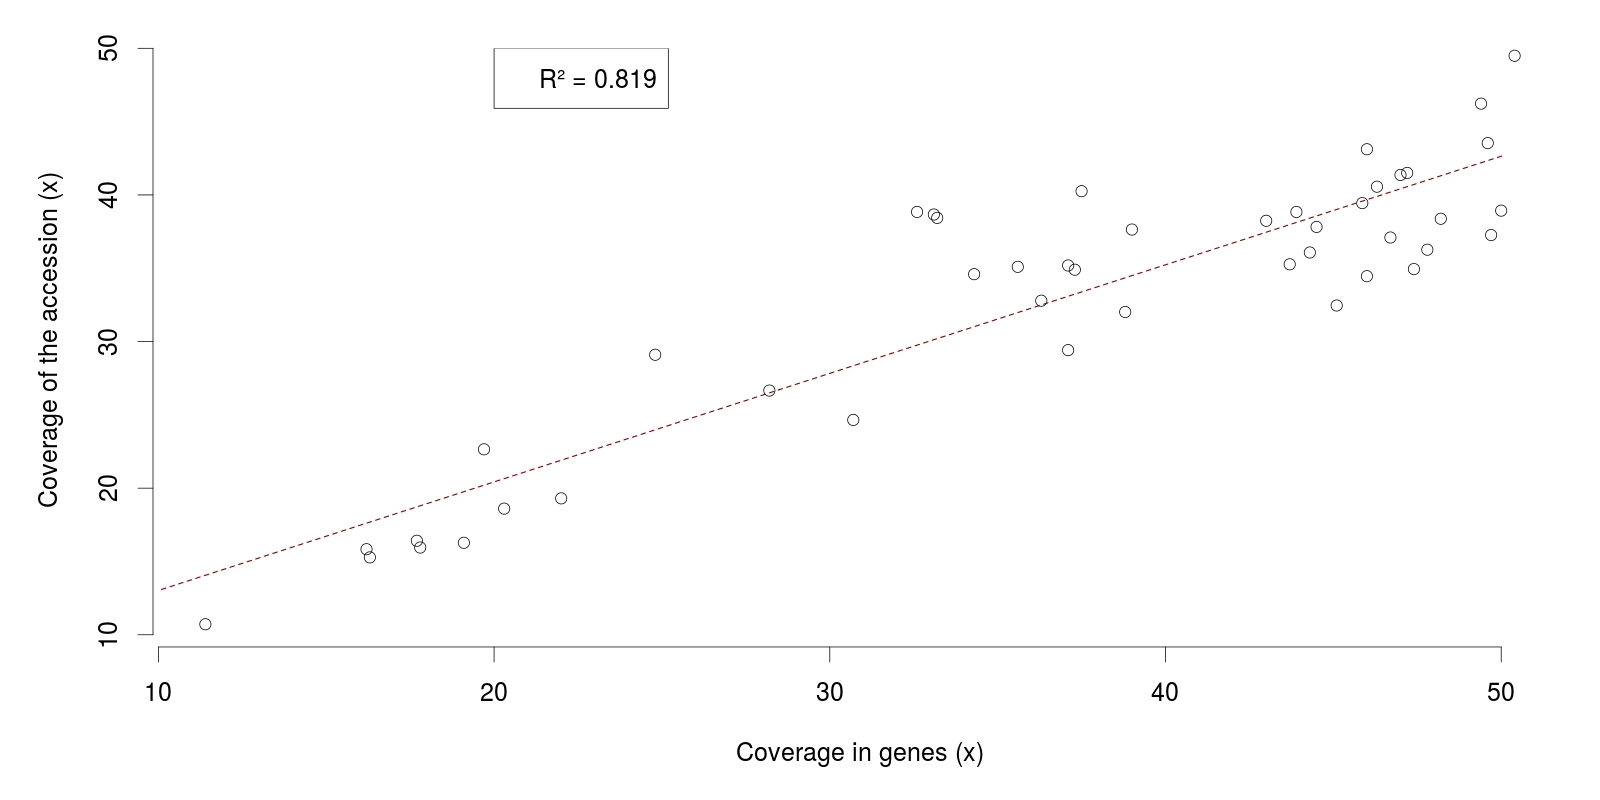
\includegraphics[scale=0.2]{Figures/Figure_11.jpg}
      \vspace{0.5cm}
      \caption{Correlation between the overall coverage and the coverage in genes} 
      \label{fig:F11}
    \footnotesize{Each dot represents an accession. The number of reads mapped in genes is a linear function of the total number of reads mapped on the 3B pseudomolecule, demonstrating that mapping is not biased towards any specific region in any of the 45 accessions.}
    \end{figure}
% - - - - - - - - - - - % % % FIGURE % % % - - - - - - - - - - - %
    \begin{figure}
    \vspace{-0.5cm}
      \centering 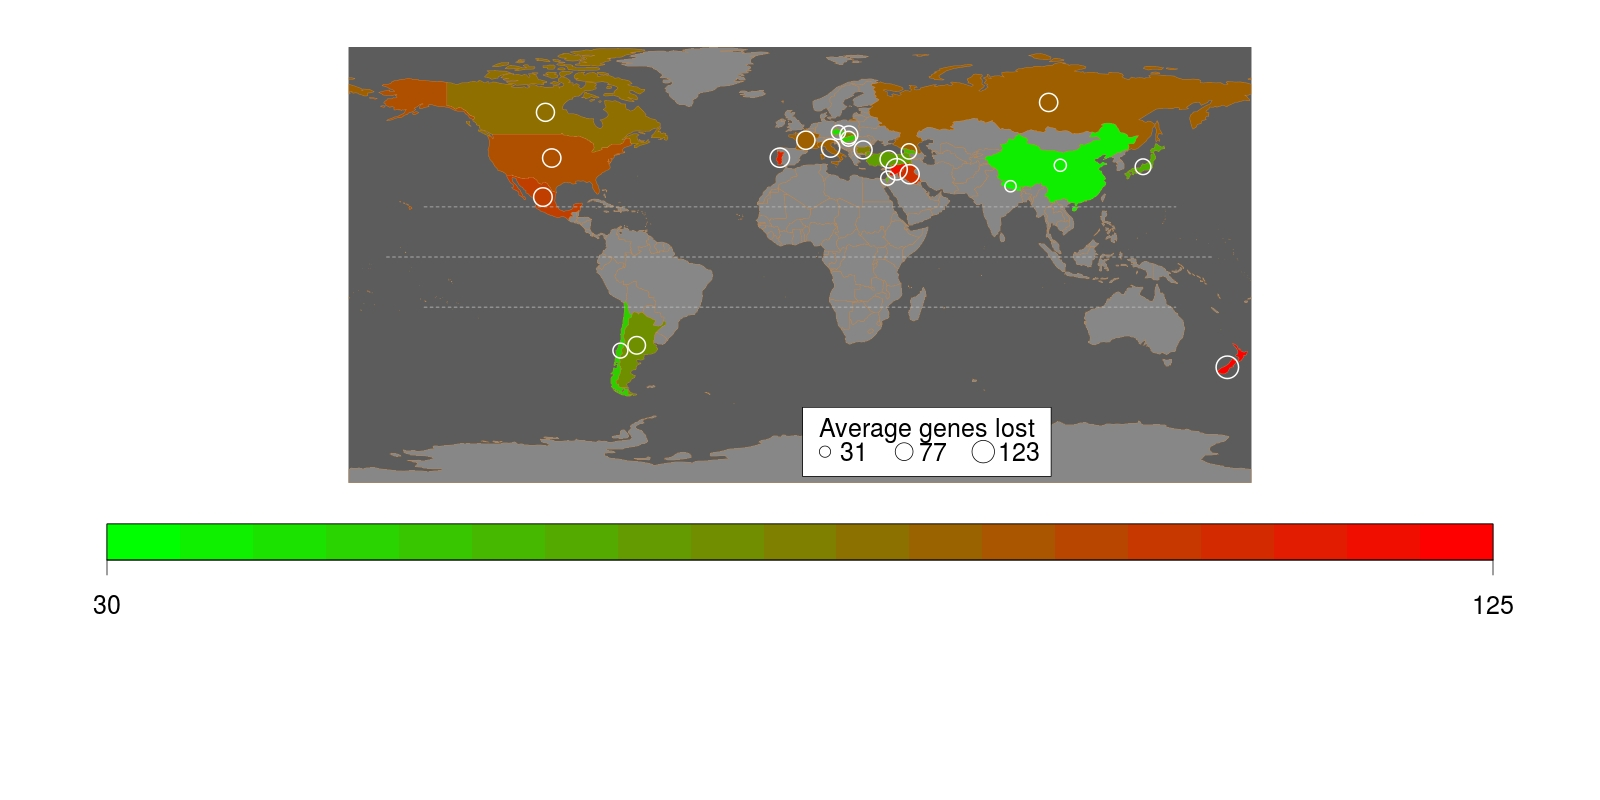
\includegraphics[scale=0.28]{Figures/Figure_12.jpg}
      \vspace{-1.5cm}
      \caption{World map of the lost genes compared to \textit{Chinese Spring}} 
      \label{fig:F12}
   \footnotesize{World map of the lost genes compared to \textit{Chinese Spring} for 44 variety coming from cross in diverse countries. The mean of lost genes by accessions coming from the same country was calculated and plot on this world map. It is clearly visible that Asian wheats are closer to \textit{Chinese Spring}, as the south-American wheats. The most divergent wheats are coming from north America, New-Zealand and middle-east with an average of 120 lost genes.}
    \end{figure}
\addtocounter{page}{-1}
\newpage
\clearpage 
% - - - - - - - - - - - % % % FIGURE % % % - - - - - - - - - - - %

To validate the absence of bias in genes coverage, the correlation between coverage in genes and along the total chromosome was assessed in figure \ref{fig:F11}. This graph allows to assess that every accession is covered equally in and out the genes, indicating no bias induced by genes during mapping process.

        \subsection{Recorded PAV and geographical data}

The total reads count in a gene, as well as the percentage of the feature covered were calculated thanks to \textit{Bedtools} package. Genes covered at less than 10\% of their total length were considered as absent in the corresponding variety. The position of each absent gene was then extracted for each accession, and was plotted on a graph (Appendix 3). Studying all varieties, the closest accession in an Israeli \textit{Triticum aestivum} wheat, \textit{N67M2} who exhibits only 24 missing genes compared to \textit{Chinese Spring}. On the other hand, the most different variety is a French \textit{Triticum aestivum} wheat, \textit{Arche} with 128 absent genes.

With an average of 71.9 genes lost per accession compared to \textit{Chinese Spring}, this panel represents 7 different species. The most divergent are the \textit{Triticum durum}, with an average of 92 genes lost per variety (sd : 22.1). \textit{Triticum macha} seem to be the closest species from the reference with an average of 49 genes lost per accession (sd : 11.3).

The number of lost genes between each accession and \textit{Chinese Spring} was then plot on a world map (Figure \ref{fig:F12}). The closest geographical origin to the reference are the Nepalese wheats (31 genes lost on average) while accessions coming from New-Zealand seem to be the most divergent from \textit{Chinese Spring} with 123 missing genes. But these data have to be taken with caution. Indeed, the country indicated is that one where the cross was done, not the one where the wheat variety came from, that's why a geographical correlation is hard to establish.

        \subsection{Lost genes and position along 3B chromosome}

Regarding the appendix 3, the different variable regions along 3B chromosome are fairly well conserved between wheat varieties. The D1 and D2 regions, from 0 to 68 and 715 to 774 Mb are the most variable, regardless of the species. The pericentromeric region is the most conserved during the evolution.

It is interesting to notice that 23 out of the 45 accessions display a small cluster of 15 genes than are often deleted, around 400 Mb. One of them is deleted in only one accession (\textit{26677}) whereas 11 genes are deleted in 14 or more varieties. 

Ten out of these eleven genes were annotated as \textit{Unknown Function} in the local database, but one of them shares homologies with a glycosyltransferase called Monogalactosyldiacylglycerol Synthase and is deleted in 23 accession on 44 in total. This gene is known to contribute to the photosynthesis process regulation by being studied thanks to the \textit{A. Thaliana} mutant \textit{mgd1-1}.

% - - - - - - - - - - - % % % FIGURE % % % - - - - - - - - - - - %
\newpage 
\thispagestyle{empty}
    \begin{figure}
      \centering 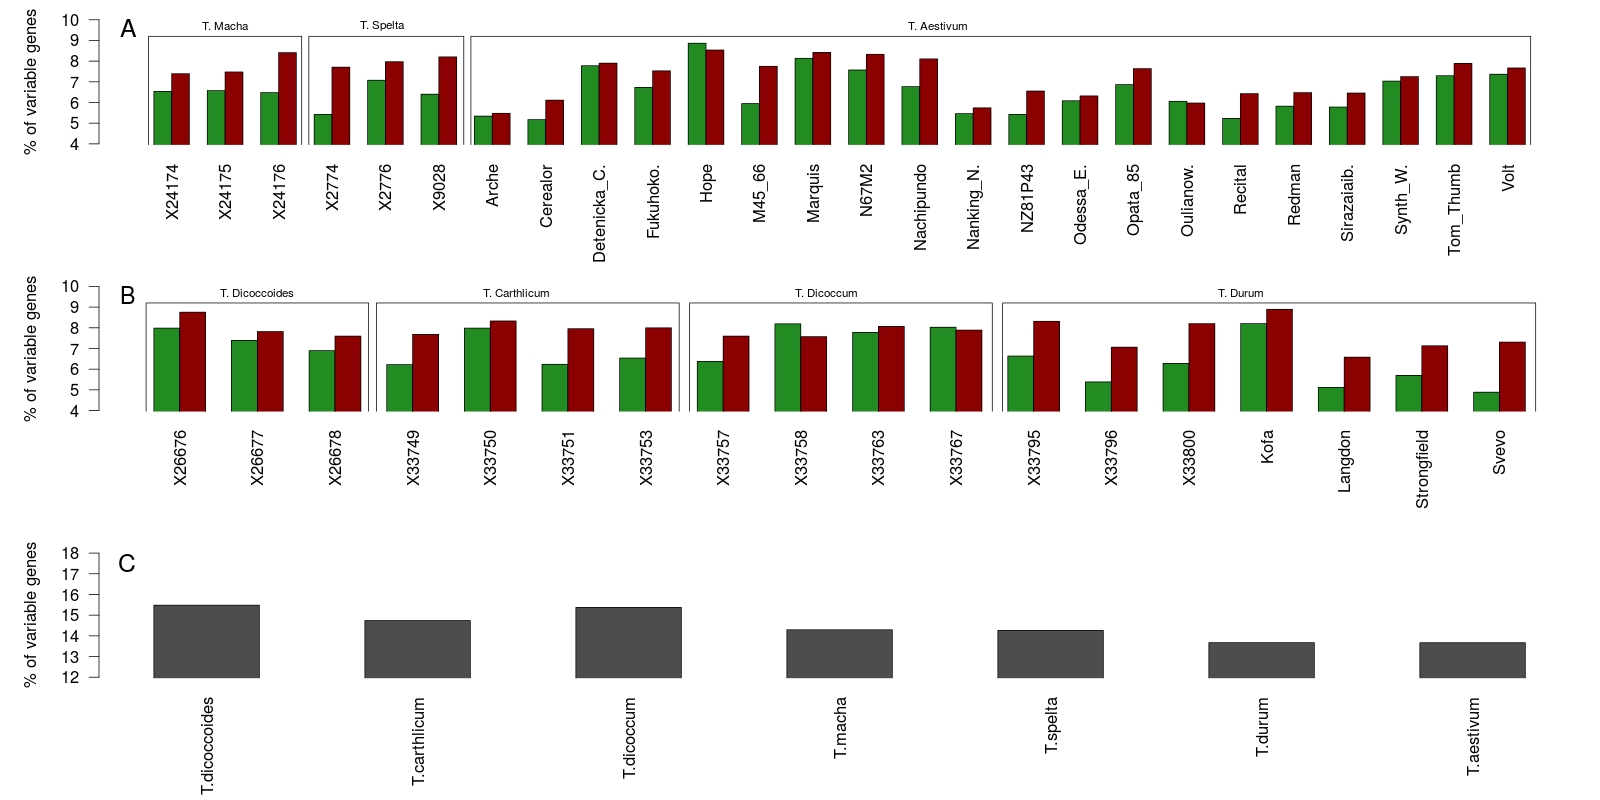
\includegraphics[scale=0.28]{Figures/Figure_13.jpg}
      \vspace{0.5cm}
      \caption{Percentage of gene structural variations compared to \textit{Chinese Spring}} 
      \label{fig:F13}
    \footnotesize{(A) Variation in hexaploid wheat accessions. Each bar represents the percentage of CNVdown (red bars) and CNVup (green bars) in each accession
    (B) Variation in hexaploid wheat accessions. Each bar represents the percentage of CNVdown (red bars) and CNVup (green bars) in each accession
    (C) Variations in \textit{Triticum} species. Each bar represents the total percentage of structural variations in each species.}
    \end{figure}
\addtocounter{page}{-1}
\newpage
\clearpage 
% - - - - - - - - - - - % % % FIGURE % % % - - - - - - - - - - - %

    \section{Variation in copy number}
    
        \subsection{Methodology development}

The most difficult part resided in the development of a normalization process to assess CNVs. Indeed, using NGS to detect CNV is usually used in human science field, and not for complex genomes such as wheat. All of the normalizations found in the literature were so adapted to human where there is no impact of the species, the number of gene per chromosome is quite low and the GC content in genes is less variable.

Several different normalization processes were tested. Finally one was selected that gave the most accurate results. As a matter of fact, it takes into account the GC percentage and the size of the gene, the coverage of the gene in \textit{Chinese Spring} and is finally $Log_{2}$ transformed for a better visualization. This process thus allows to use the number of mapped reads in a feature to detect CNV in complex and larges genomes, such as wheat.
    
        \subsection{Threshold, where is there a CNV ?}

Following the normalization process of numbers of reads mapped in each gene, every value from an accession is directly comparable to the \textit{Chinese Spring}'s value. Variations in copy number were defined using the following thresholds:

\vspace{0.5cm}
$T_{low} = \bar{X}_{accession} - SD$ 
\vspace{0.5cm}

$T_{up} = \bar{X}_{accession} + SD$
\vspace{0.5cm}

With $\bar{X}_{accession}$ being the average value for a given accession (\textit{i.e} the mean of the normalized number of read from a given accession, which have mapped in each gene) and SD the standard deviation. If a gene from a variety have a value smaller than $T_{low}$, a decrease in copy number is expected (deletion), hereafter referred to as \textit{CNVdown}. If greater than $T_{up}$, an increase is expected (duplication), hereafter referred to as \textit{CNVup}.

Thanks to these thresholds, the PAV data were verified. Indeed, every gene marked as \textit{absent} (covered by less than 10\% during mapping) was also found as \textit{CNVdown} with this methodology.

        \subsection{Increases, decreases, recorded variations}
        
Regarding all of the 44 accessions compared with \textit{Chinese Spring}, deletion was more important than duplication, with 7.5 and 6.6\% of the gene content respectively on average (Figure \ref{fig:F13} A and B). The species exhibiting the more deletions is the \textit{Triticum dicoccoides}, with an average of 585 CNVdown. 

% - - - - - - - - - - - % % % FIGURE % % % - - - - - - - - - - - %
\newpage 
\thispagestyle{empty}
    \begin{figure}
      \centering 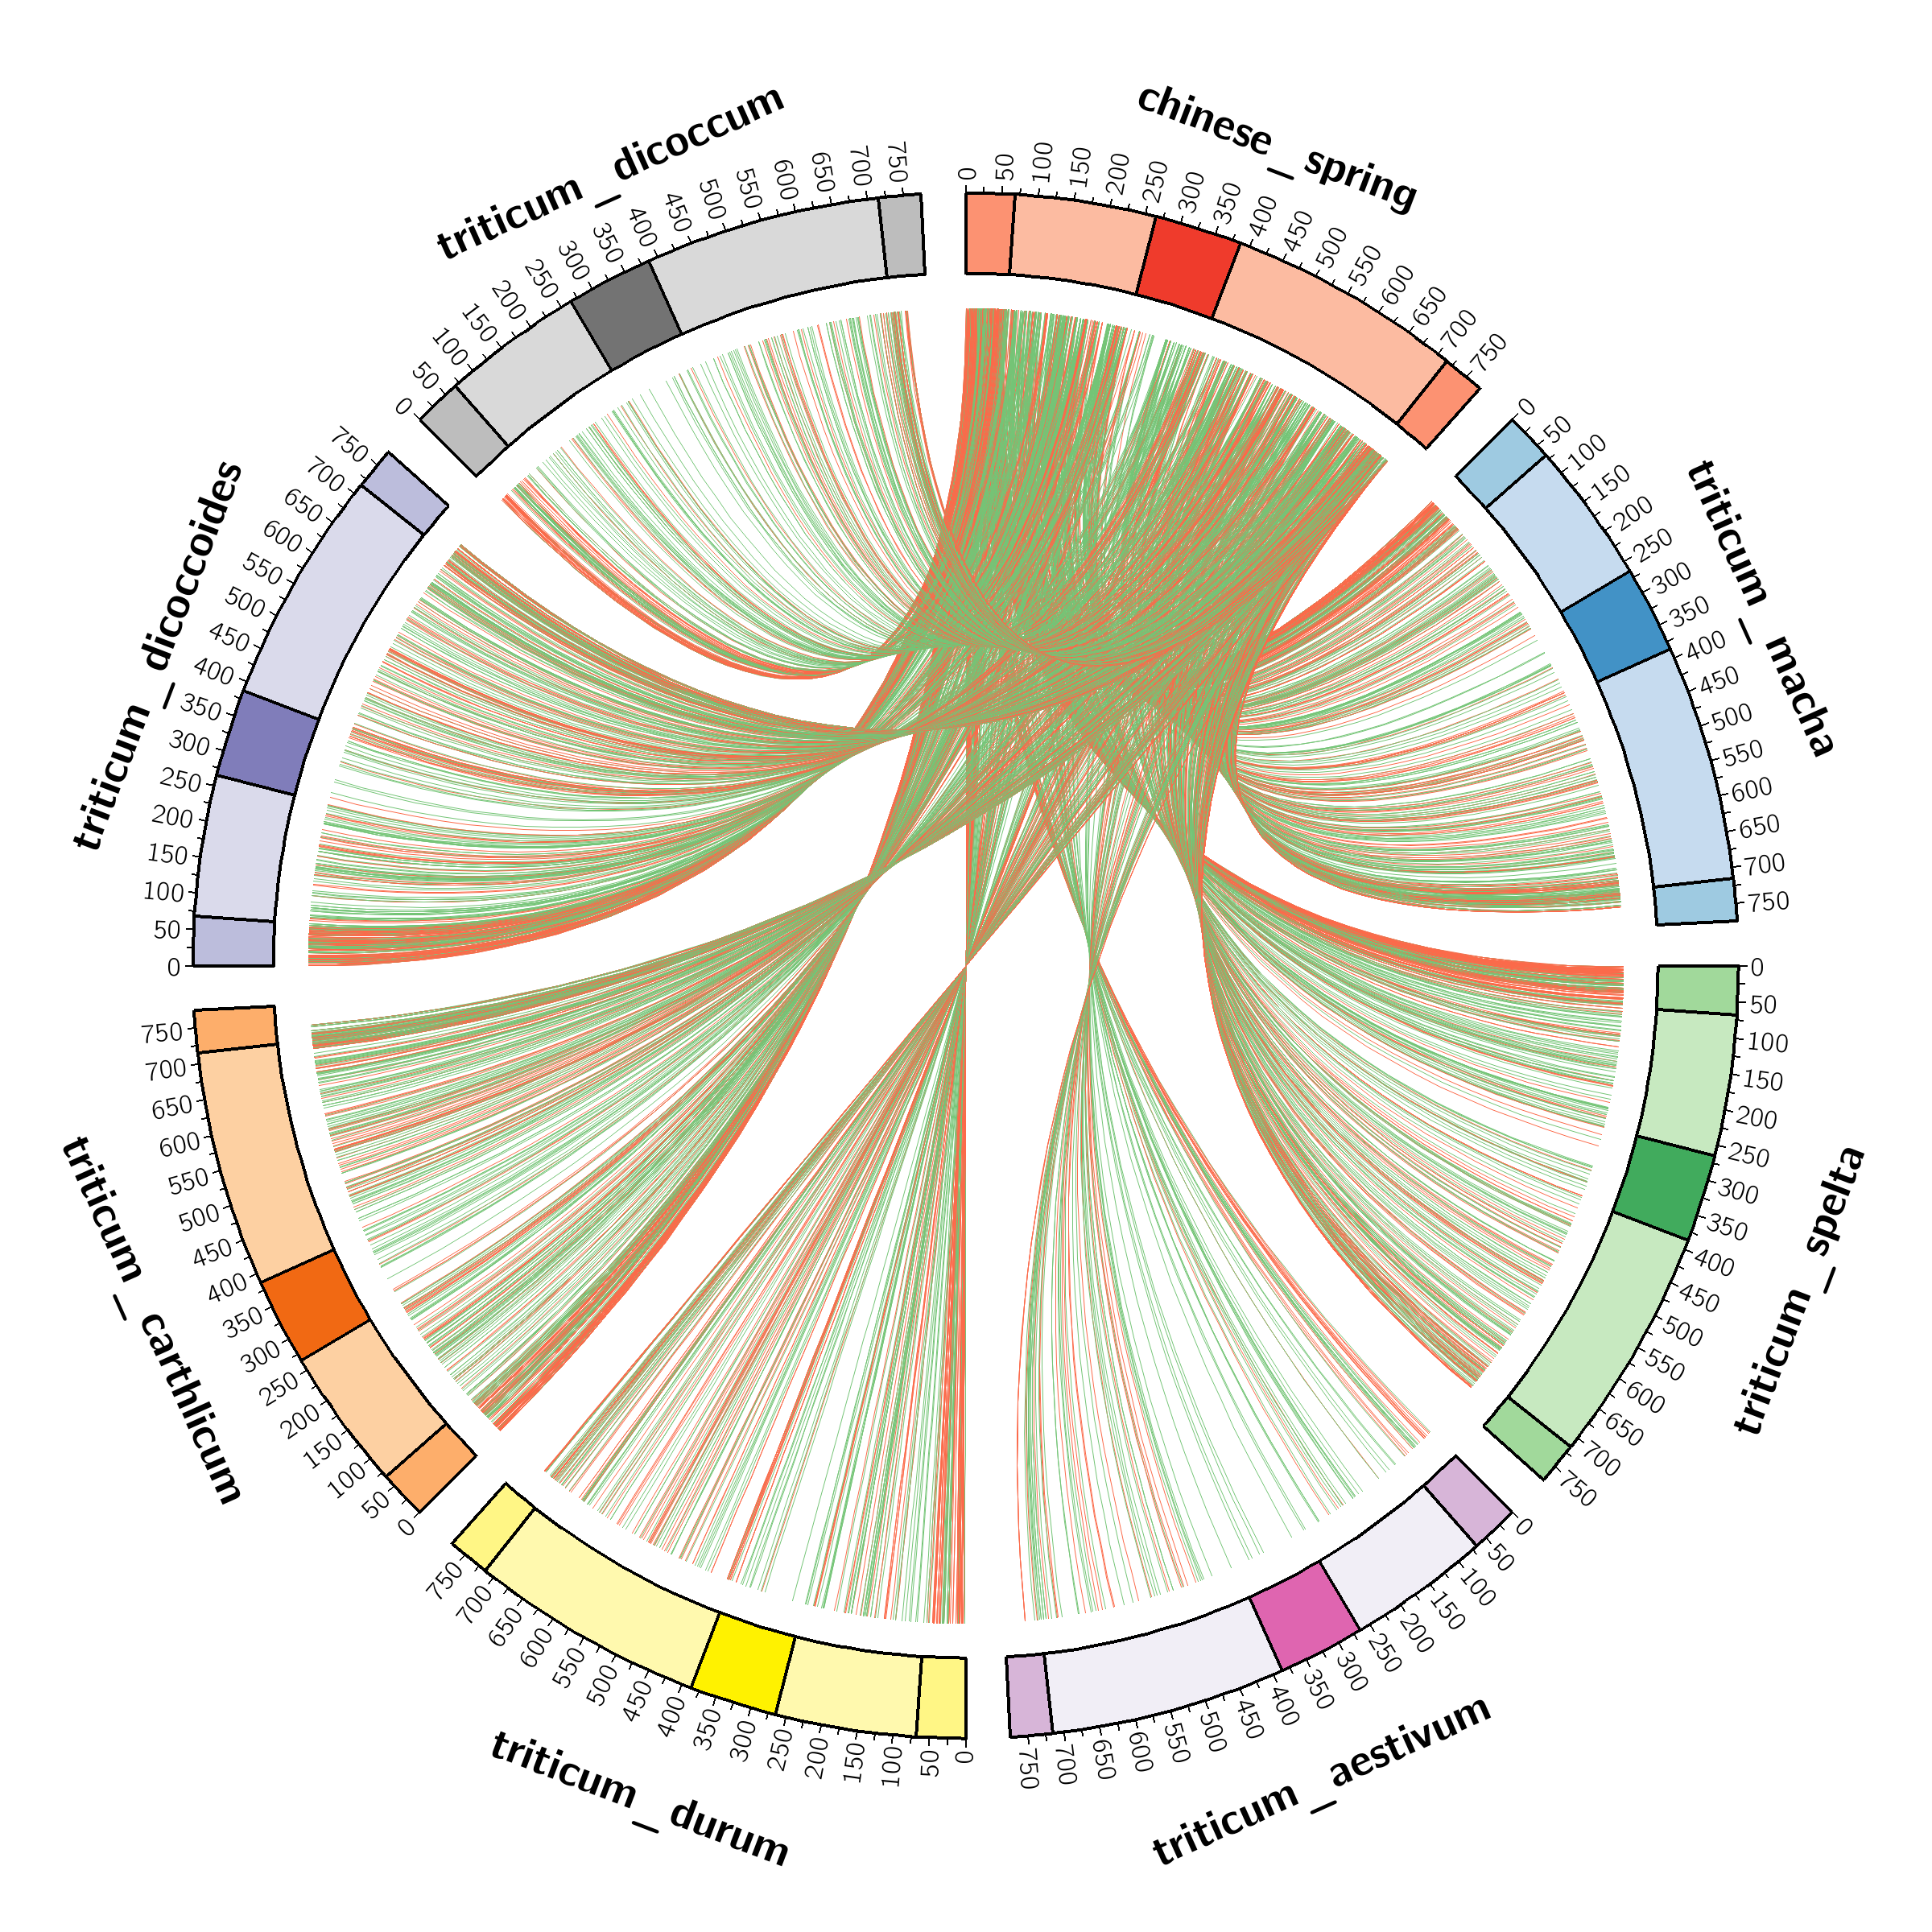
\includegraphics[scale=0.09]{Figures/Figure_14.png}
      \vspace{0.5cm}
      \caption{Circos diagram illustrating the distribution of SVs along 3B chromosomes} 
      \label{fig:F14}
    \footnotesize{Circos plot of the variations shared between every members of a subgroup and \textit{Chinese Spring}. The losses (red lines) and gains (green lines) in copy number are really higher in the distal regions for every subfamily. The \textit{T. aestivum} show the smallest number of variations, as expected.}
    ~
    \end{figure}
% - - - - - - - - - - - %
    \begin{figure}
    \vspace{-0.01cm}
      \centering 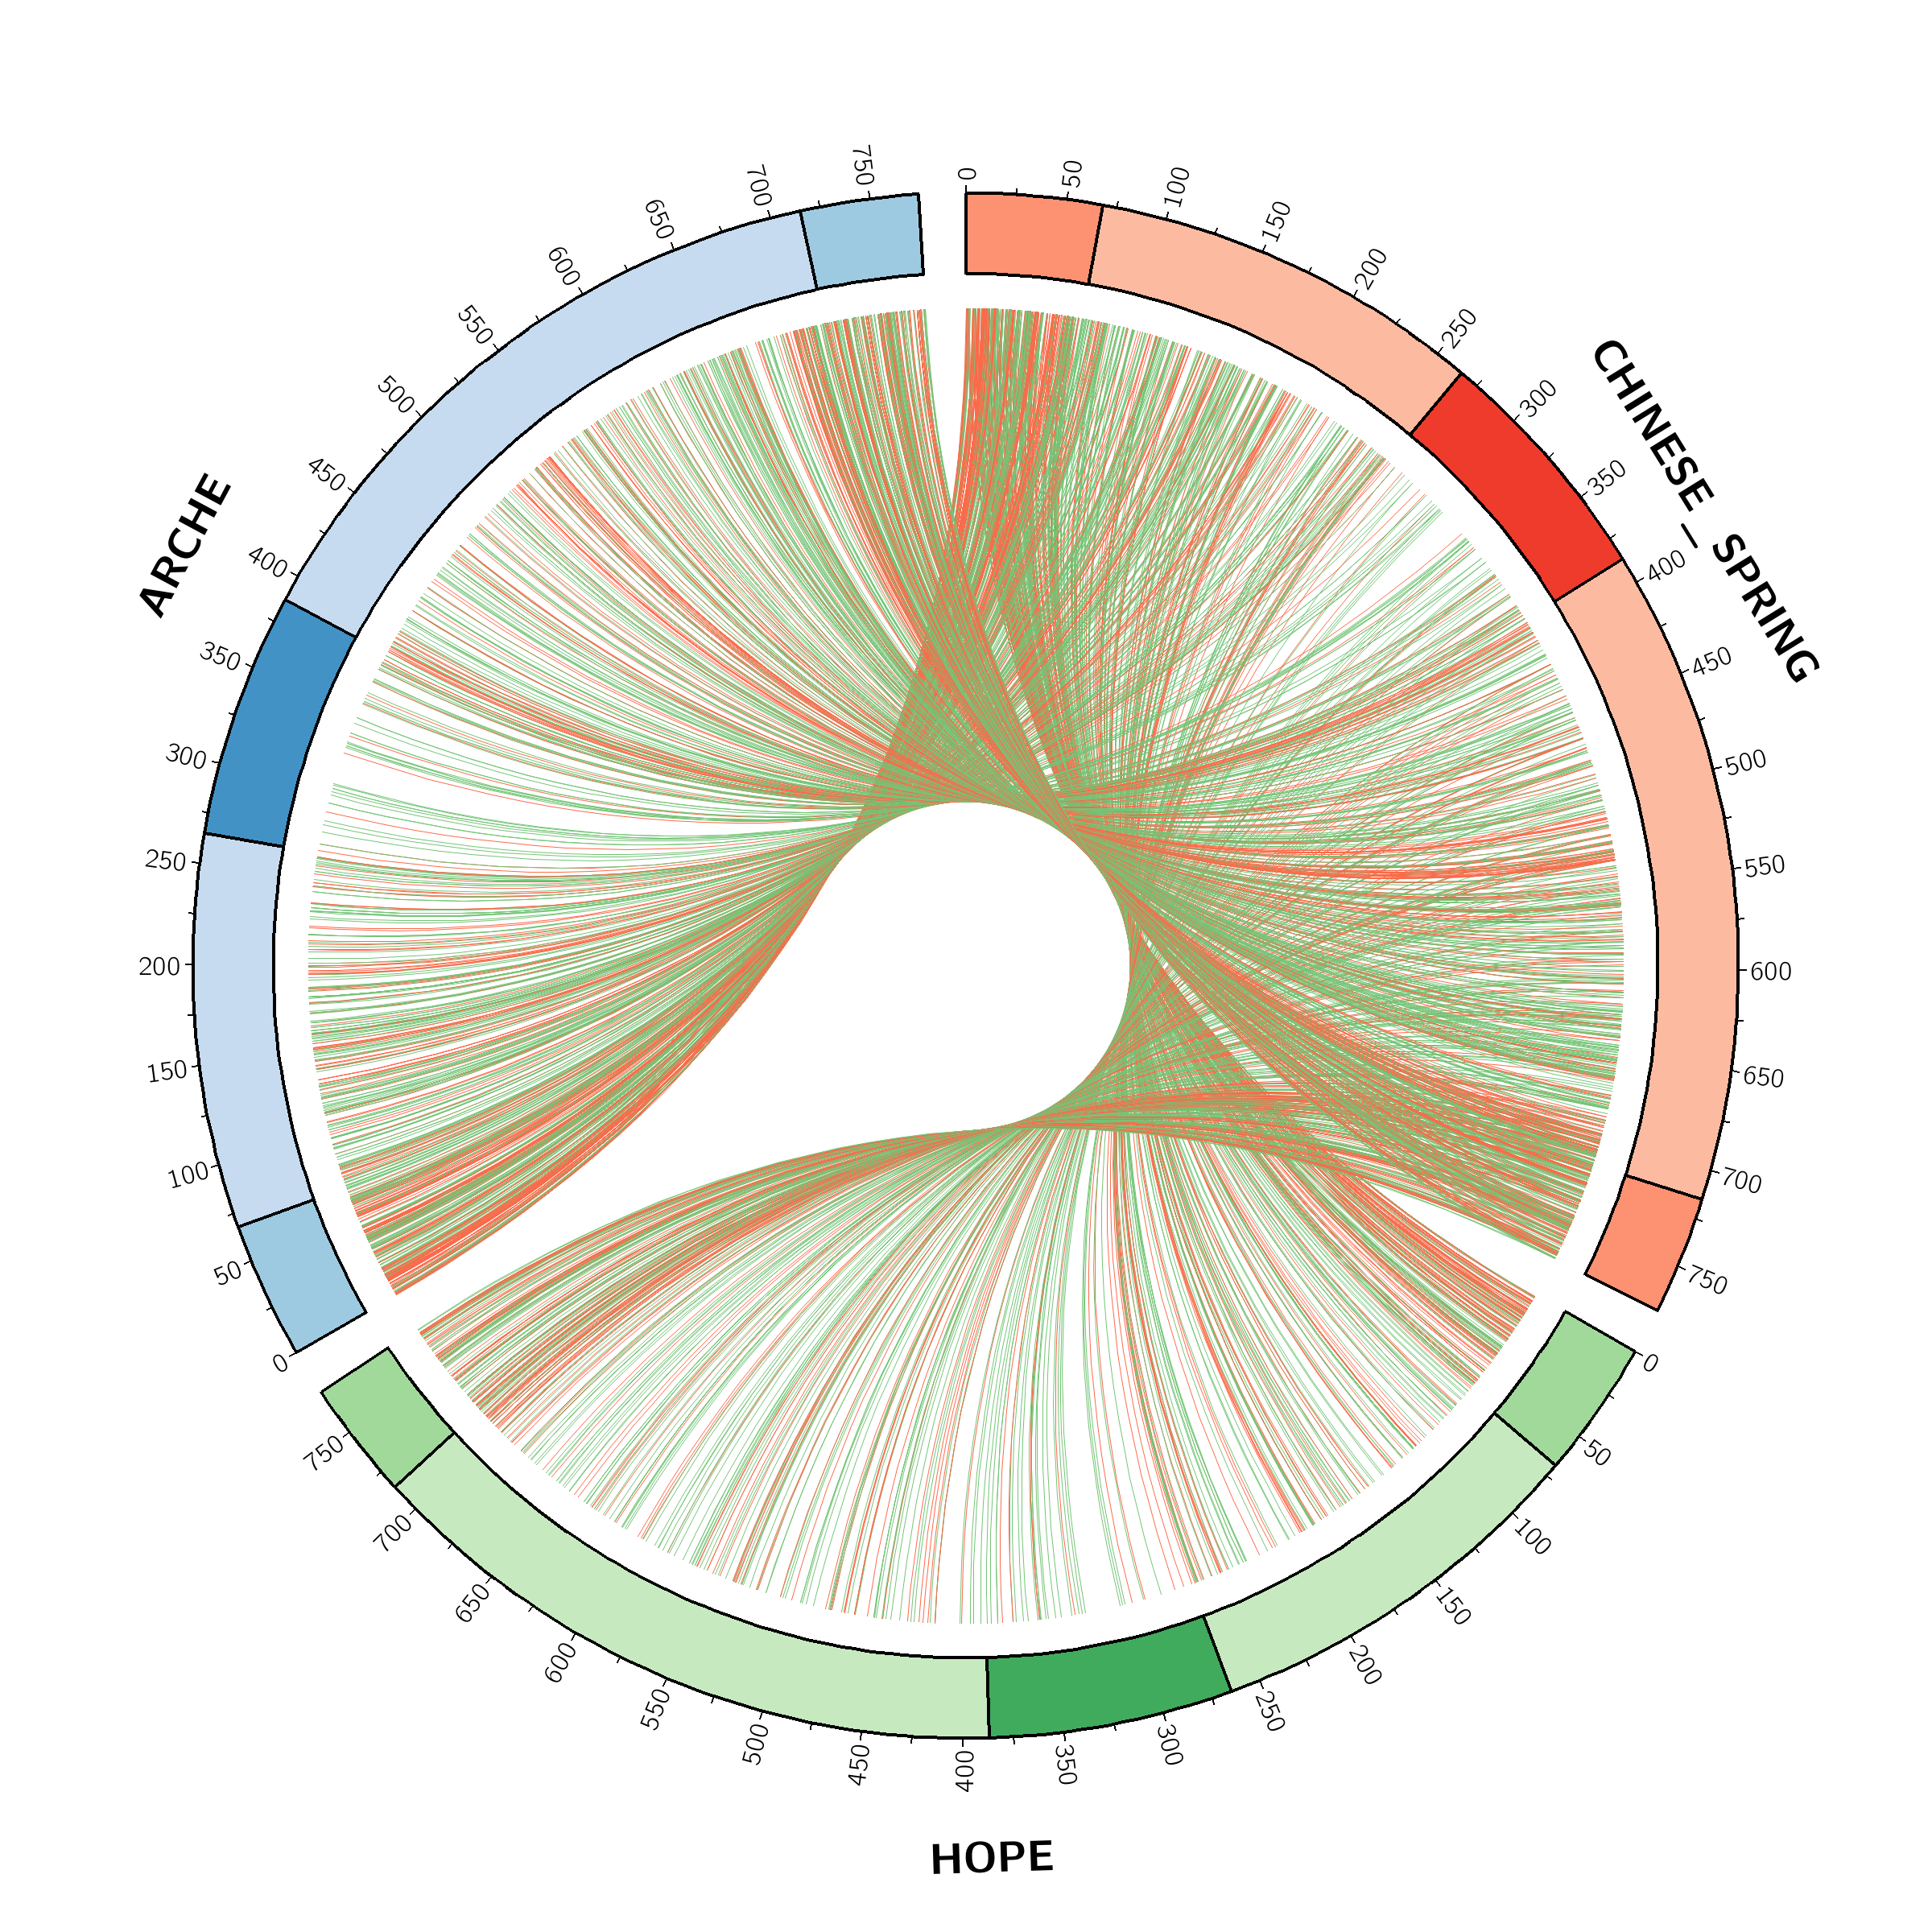
\includegraphics[scale=0.09]{Figures/Figure_15.png}
      \vspace{0.5cm}
      \caption{Representation of CNVs between \textit{Chinese Spring} and closest/farthest wheats}
      \label{fig:F15}
    \footnotesize{Regarding CNV events, \textit{Hope} is the most divergent wheat (17.4\% of genic variation) and \textit{Arche} the closest (10.82\%) compared to \textit{Chinese Spring}. It is visible that the gains in copy number (green lines) and the loss (red lines) happen more often in the distal regions compared to the pericentromeric one. A small area in the centromer show no variations at all and can contain the most important genes for wheat survival.}
    \end{figure}
\addtocounter{page}{-1}
\newpage
\clearpage 
% - - - - - - - - - - - % % % FIGURE % % % - - - - - - - - - - - %

The \textit{Triticum dicoccum} seem to be the most divergent in duplication with an average of 552 CNVup. The closest species regarding the decrease in copy number is the other \textit{Triticum aestivum} (518 CNVdown in average) and the \textit{Triticum durum} for the increase (438 CNVup).

Differences are visible even regarding the ploidy level. By taking in account both duplication and deletions, it is clearly visible that hexaploid (AABBDD) wheats have less events  than tetraploids (AABB) wheats (Figure \ref{fig:F13} C). The three hexaploid species from the panel have 14.07\% of variable genes on average compared to \textit{Chinese Spring} (SD: 0.35) and the closest species are the \textit{T. spelta} with 14.26\% of their genes different (as expected, \textit{T. aestivum} have an average of 13.67\% of variable genes compared to \textit{Chinese Spring}). The four tetraploid species have an average of 14.8\% of variables genes (SD: 0.83) and the most different from the reference are the \textit{T. dicoccoides} with up to 15.5\% of their genes divergent. Surprisingly, the \textit{T. durum}, tetraploids, seem to be more close to \textit{T. aestivum} than the other hexaploids. But it is visible on the graph 13B that \textit{Langdon}, \textit{Strongfield} and \textit{Svevo} have less duplication events compared to the others tetraploids, thus pulling the mean.

A circos plot of the variation between \textit{Chinese Spring} and the 7 species was also designed (Figure \ref{fig:F14}). The distal parts of the 3B chromosome are always more variable than the pericentromeric one. It is also clearly visible than the \textit{Chinese Spring} have less genic variation with the \textit{T. aestivum}, as expected.

By considering each variety individually instead of the entire species, the two extremes in terms of deletions are \textit{Arche} (\textit{Triticum aestivum}) (398 genes) and \textit{Kofa} (\textit{Triticum durum}) (646 genes). For duplications, the most different accession is \textit{Hope} (\textit{Triticum aestivum}), with 644 CNVup, while  \textit{Svevo} (\textit{Triticum durum}) displays only 355.

Regarding all of the recorded variations, \textit{Arche} seems to be the closest wheat to \textit{Chinese spring} with 10.8\% of the gene content variable (398 CNVdown and 388 CNVup) (Figure \ref{fig:F15}). The most divergent, \textit{Hope}, is variable at 17.4\%  (620 CNVdown and 644 CNVup). On the Circos representation, it become obvious that the distal parts of the 3B chromosome are the main targets of these modifications. A short deletion cluster is even visible around 550 Mb for \textit{Arche}.

        \subsection{Using the assembly, where does it vary?}
        
The percentages of genes having more or less copies compared to \textit{Chinese Spring} in a 10 Mb sliding windows were plotted along the 3B chromosome (Appendix 4). First of all, it is clearly visible that the distal regions are more polymorphic than the pericentromeric region for all accessions. A region, around 400 Mb, is more variable compare to adjacent ones, regarding the deletions or duplications. This position was also found on PAV study, representing a short deletion cluster. 

% - - - - - - - - - - - % % % FIGURE % % % - - - - - - - - - - - %
\newpage 
\thispagestyle{empty}
    \begin{figure}
    \vspace{-2cm}
      \centering 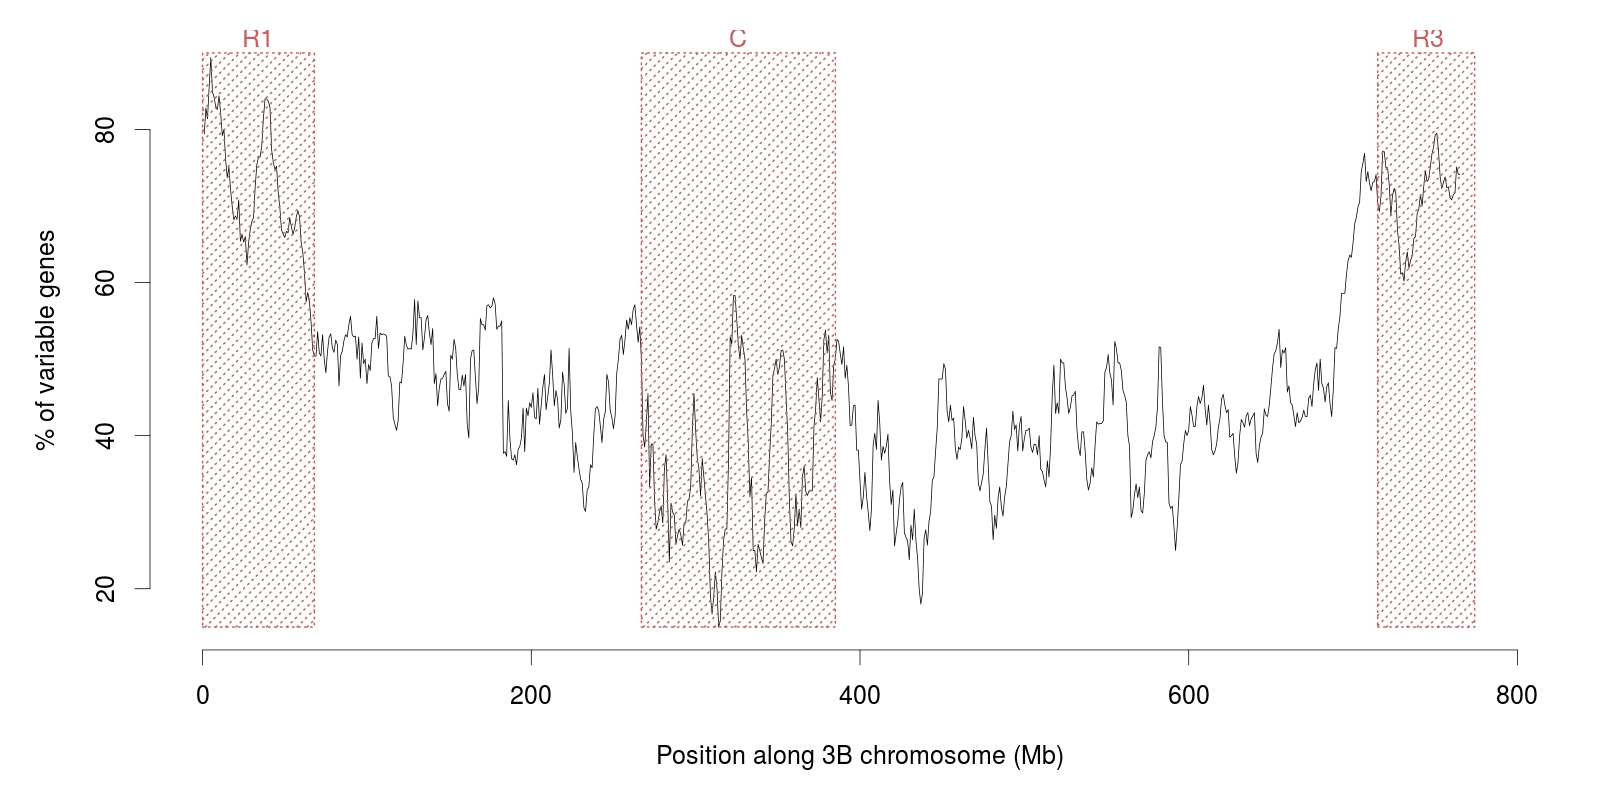
\includegraphics[scale=0.19]{Figures/Figure_16.jpg}
      \vspace{0.5cm}
      \caption{Distribution of the percentage of variable genes along chromosome 3B} 
      \label{fig:F16}
    \footnotesize{The average percentage of CNV was calculated in a 10-Mb sliding window (step 1 Mb).  The red dashed areas are the chromosomal regions R1, C and R3 defined by Choulet \textit{et al.}.}
    \end{figure}
% - - - - - - - - - - - % % % FIGURE % % % - - - - - - - - - - - %
    \begin{figure}
    \vspace{-1cm}
      \centering 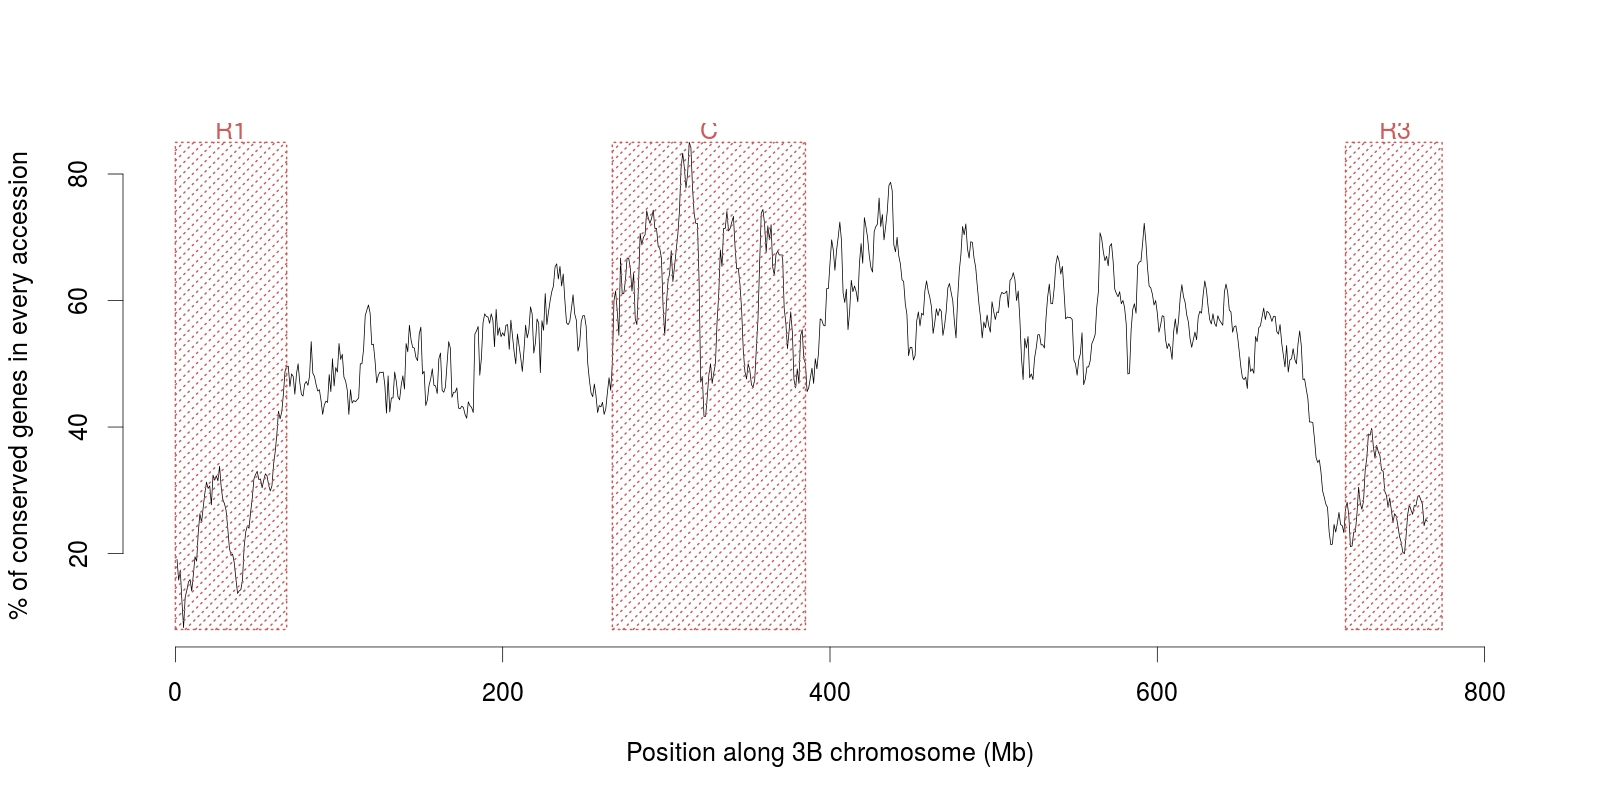
\includegraphics[scale=0.19]{Figures/Figure_17.jpg}
      \vspace{0.5cm}
      \caption{Distribution of the percentage of non variable genes along chromosome 3B}
      \label{fig:F17}
    \footnotesize{The average percentage of genes showing no variation among the panel was calculated in a 10-Mb sliding window (step 1 Mb).  The red dashed areas are the chromosomal regions R1, C and R3 defined by Choulet \textit{et al.}.}
    \end{figure}
% - - - - - - - - - - - % % % FIGURE % % % - - - - - - - - - - - %
    \begin{figure}
    \vspace{-1cm}
      \centering 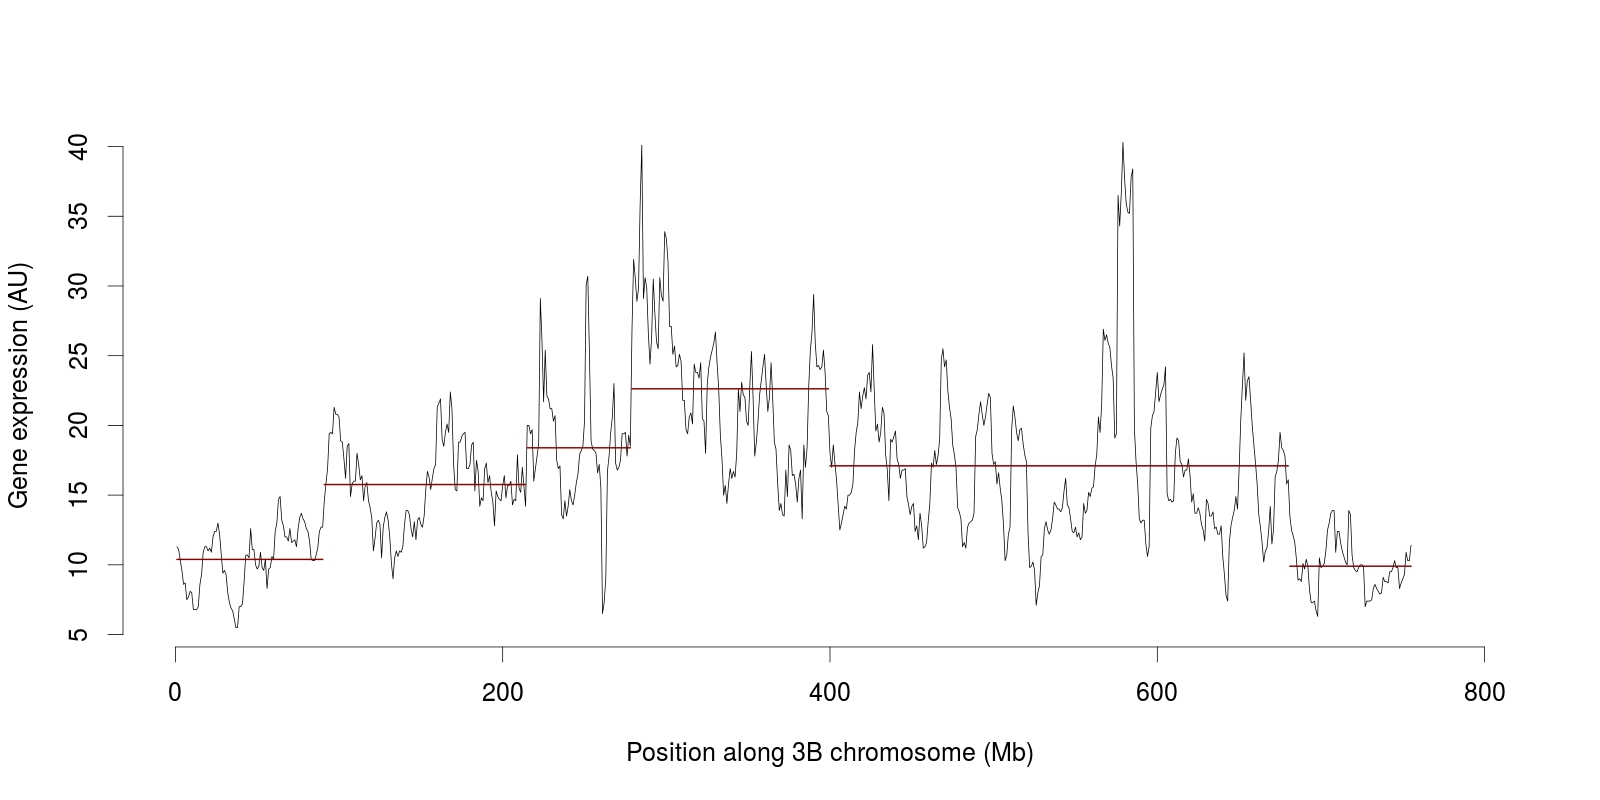
\includegraphics[scale=0.19]{Figures/Figure_18.jpg}
      \vspace{0.5cm}
      \caption{Genic expression depending of the position on the 3B chromosome}
      \label{fig:F18}
   \footnotesize{ Genic expression was calculated with the ratio between the average expression in 15 condition and the number of condition where the gene is transcribed. The segmentation of this graph shows 6 areas along the 3B (red lines), indicating different expression patterns. Genes located in R1/R3 regions are expressed in fewer condition and in at a lower rate. Those in the C regions are constitutively transcribed, strengthening the idea of a core genome located in the middle of the 3B chromosome. (AU: arbitrary units).}
    \end{figure}
\addtocounter{page}{-1}
\newpage
\clearpage 
% - - - - - - - - - - - % % % FIGURE % % % - - - - - - - - - - - %

The percentage of variable genes in at least one accession in a 10 Mb-windows was plotted (Figure \ref{fig:F16}). It confirms that the D1 and D2 regions are more variable than pericentromeric one (from 50 to 80\% of variable genes versus $\approx$ 40\%). By taking this information in account, it is possible to rise a question about the importance of every part of the 3B chromosome. Some of them, around C region, seem to be more conserved, indicating a greater importance for a proper development of the individual. 

    \section{Wheat gene set, a story about evolution} 
    
        \subsection{Study of the core genome}
        
In an organism, its gene set is responsible of the ability to survive in an environment. Some gene, belonging to the \textit{core genome}, are mandatory for the proper development and their deletion may be lethal for the individual. Other, composing the \textit{dispensable genome} were acquired during evolution by a family, a specie or an individual, as a result of adaptation.

By studying variations on a wheat gene set, it is now possible to search for its \textit{core genome}. Thus, 3,243 genes show no variations in any individual of the panel. By looking at their position on figure \ref{fig:F17}, it is obvious that the percentage of invariable genes is higher in the pericentromeric region ($\approx$ 60\%) than in the distal ones ($\approx$ 25 \%). Thus, it occurs that genes located at the ends of the 3B are more variable in copy number than those around the C region. 

By using the RNA-seq results produced by the lab, the expression of the total gene set of the 3B chromosome from \textit{Chinese Spring} was studied. The expression of the 7,264 genes was recorded on 5 tissues and 3 development conditions (15 in total). Their mean expression level was plotted on chromosome 3B (figure \ref{fig:F18}). It showed that the genes in the pericentromeric region tend to have higher expression level and expression breadth (data not shown) than those located on the distal parts of the chromosome, suggesting their potential role in house-keeping functions.

Thus, it becomes obvious that the 3,243 genes of the \textit{core genome} are more often transcribed and mainly located in the pericentromeric region of the 3B chromosome. Out of the 4,021 remaining genes, 728 are absent in at least one accession and correspond to the \textit{dispensable genome}. The remaining 3,293 genes are variable in copy number in one accession or more and form the \textit{variable genome}. Such variations in copy number are likely to play a role in the specific adaptation of individuals or species to a specific environment  or to lead intrinsic properties.

% - - - - - - - - - - - % % % FIGURE % % % - - - - - - - - - - - %
\newpage 
\thispagestyle{empty}
    \begin{figure}
    \vspace{-1cm}
      \centering 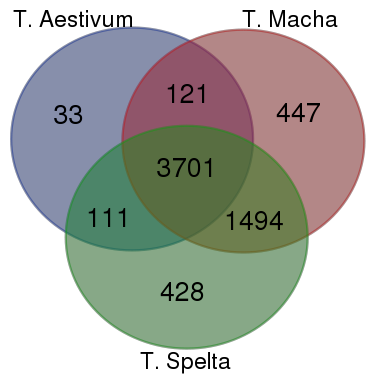
\includegraphics[scale=0.3]{Figures/Figure_19.png}
      \vspace{0.3cm}
      \caption{Venn diagram of shared genes between three hexaploid wheat species} 
      \label{fig:F19}
    \footnotesize{Number of genes shared between \textit{T. aestivum}, \textit{T. macha} and \textit{T. spelta} are indicated.}
    \end{figure}
% - - - - - - - - - - - %
    \begin{figure} 
    \vspace{-1.2cm}
      \centering 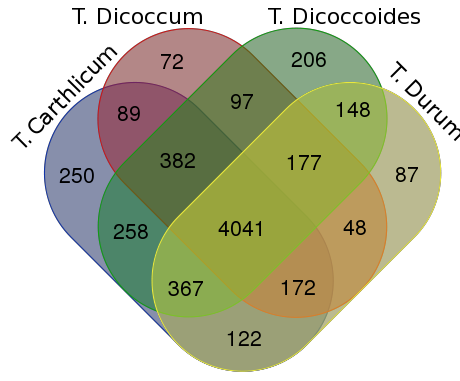
\includegraphics[scale=0.3]{Figures/Figure_20.png}
      \vspace{0.3cm}
      \caption{Venn diagram of shared genes between four tetraploid wheat species} 
      \label{fig:F20}
    \footnotesize{Number of genes shared between \textit{T. durum}, \textit{T. carthlicum}, \textit{T. dicoccum} and \textit{T. dicoccoides} are indicated.}
    \end{figure}
% - - - - - - - - - - - %
    \begin{figure}
    \vspace{-1.2cm}
      \centering 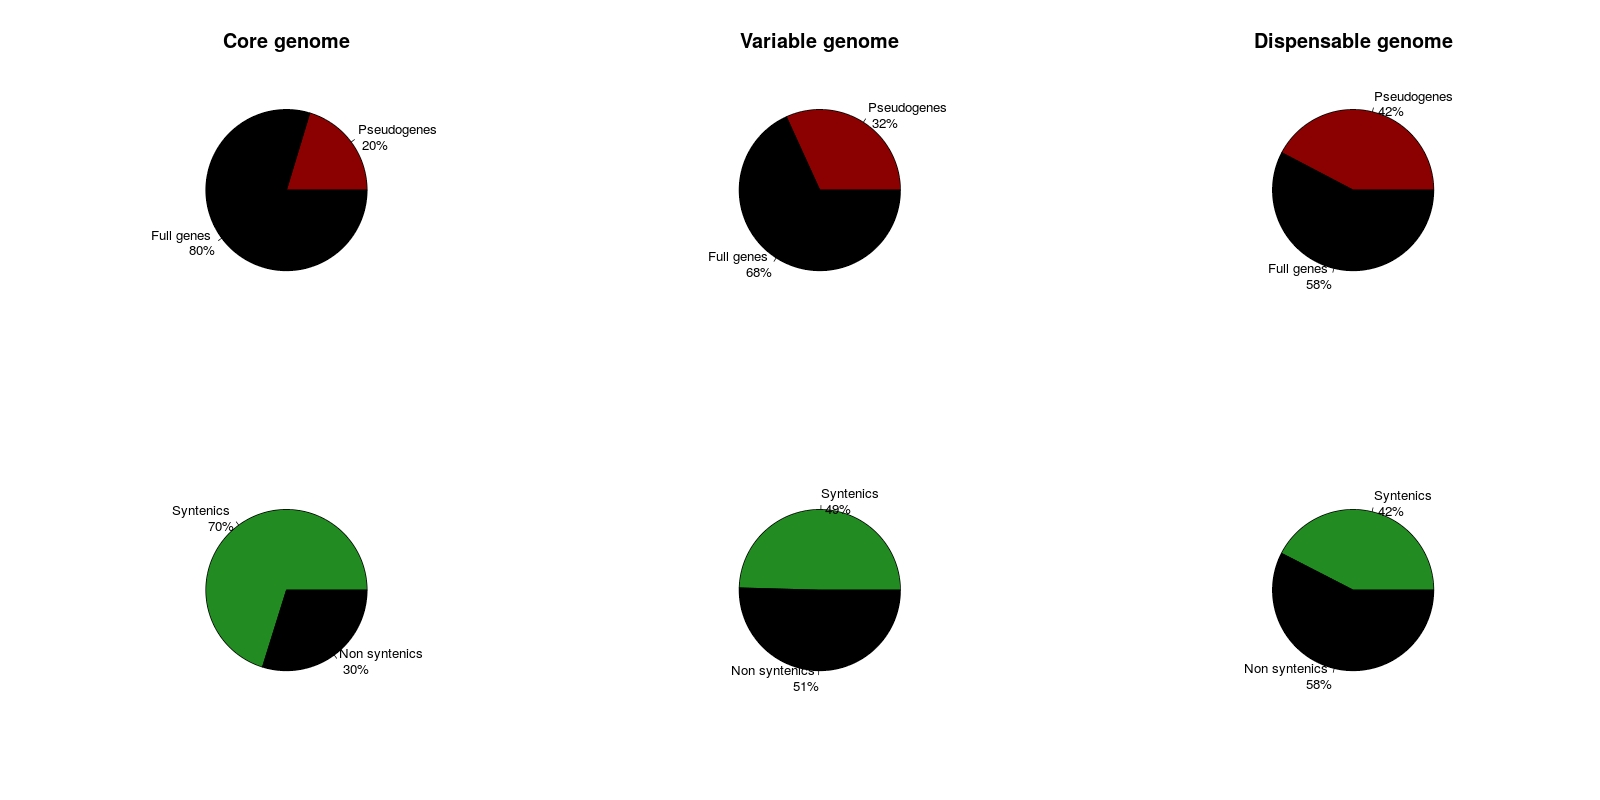
\includegraphics[scale=0.28]{Figures/Figure_21.jpg}
      \caption{Proportion of gene categories in the \textit{Triticum} genomes} 
      \label{fig:F21}
    \footnotesize{Upper part: proportion of syntenic (black) and nonsyntenic (red) genes in the core, variable and dispensable genomes of \textit{Triticum}.
    
    Lower part: proportion of full genes (black) and pseudogenes / gene fragments (green) in the core, variable and dispensable genomes of \textit{Triticum}.}
    \end{figure}
\addtocounter{page}{-1}
\newpage
\clearpage 
% - - - - - - - - - - - % % % FIGURE % % % - - - - - - - - - - - %

It was also checked how genes could be shared between the different species depending on their ploidy level. The figure \ref{fig:F19} shows how  conserved genes are shared among hexaploids. Thus, 3701 genes seem to be shared by all hexaploid species. 

The \textit{T. macha} and \textit{T. spelta} share a large amount of 1,494 genes compared to those shared with the \textit{T. aestivum}. The tetraploid species, on figure \ref{fig:F20}, shared together 4,041 genes, with 258 between \textit{T. carthlicum} and \textit{T. dicoccoides} and 48 between \textit{T. durum} and \textit{T. dicoccum}.

        \subsection{Synteny, non synteny?}
        
A syntenic gene is defined by its simultaneous presence on two or more loci in the same chromosome, in regions derived from a common ancestor. Based on previous results from the group, genes were classified as being syntenic or nonsyntenic. So, what about the core fraction of the wheat genome ?

By looking at the proportion of syntenic or non-syntenic genes in the previously defined core genome (3,243 genes), it is clear that syntenic genes are more conserved among the wheat species (2,276 genes, 70\%) than the non-syntenic (967 genes, 30\%). This can be linked to the global proportion of 73\% of syntenic genes along the 3B chromosome. However, it is visible on figure \ref{fig:F21} that the proportion of syntenic genes decrease for the variable genome (49\%) and even more for the dispensable genome (42\%). 

A second analysis was performed on a filtered gene set in which species-specific genes and pseudogenes and gene fragments have been removed. Thus, no differences were visible, regardless the different species. Indeed, every defined subgenome contains 70\% of syntenic genes and 30\% of non-syntenic genes. This strongly suggests that pseudogenes and gene fragments might be responsible for the difference between core and variable genomes. To assess whether this is the case or not, the proportion of syntenic and non-syntenic genes was calculated among the non-variable genes (Figure \ref{fig:F22}). Thus, it was showed that the proportion of syntenic/non-syntenic in the \textit{core genome} remain steady among the species, indicating a large amount of pseudogenes in the R1/R3 regions. The fact than \textit{T. aestivum} are lower than the others is due to the size of this subgroup (20 members), which is higher than for others species (ranged from 3 to 7). It is harder to find genes which remain constant in every members of the subgroup.

    \section{A phylogenetic story}
        
Based on the matrix, a clustering was performed with \textit{pvclust} R package (Figure \ref{fig:F23}). This phylogenetic tree shows a clear separation between \textit{T. aestivum} and other species. Surprisingly, \textit{T. macha} and \textit{T. spelta} were found to be more related to tetraploid species than to \textit{T. aestivum}. 

% - - - - - - - - - - - % % % FIGURE % % % - - - - - - - - - - - %
\newpage 
\thispagestyle{empty}
    \begin{figure}
    \vspace{-0.8cm}
      \centering 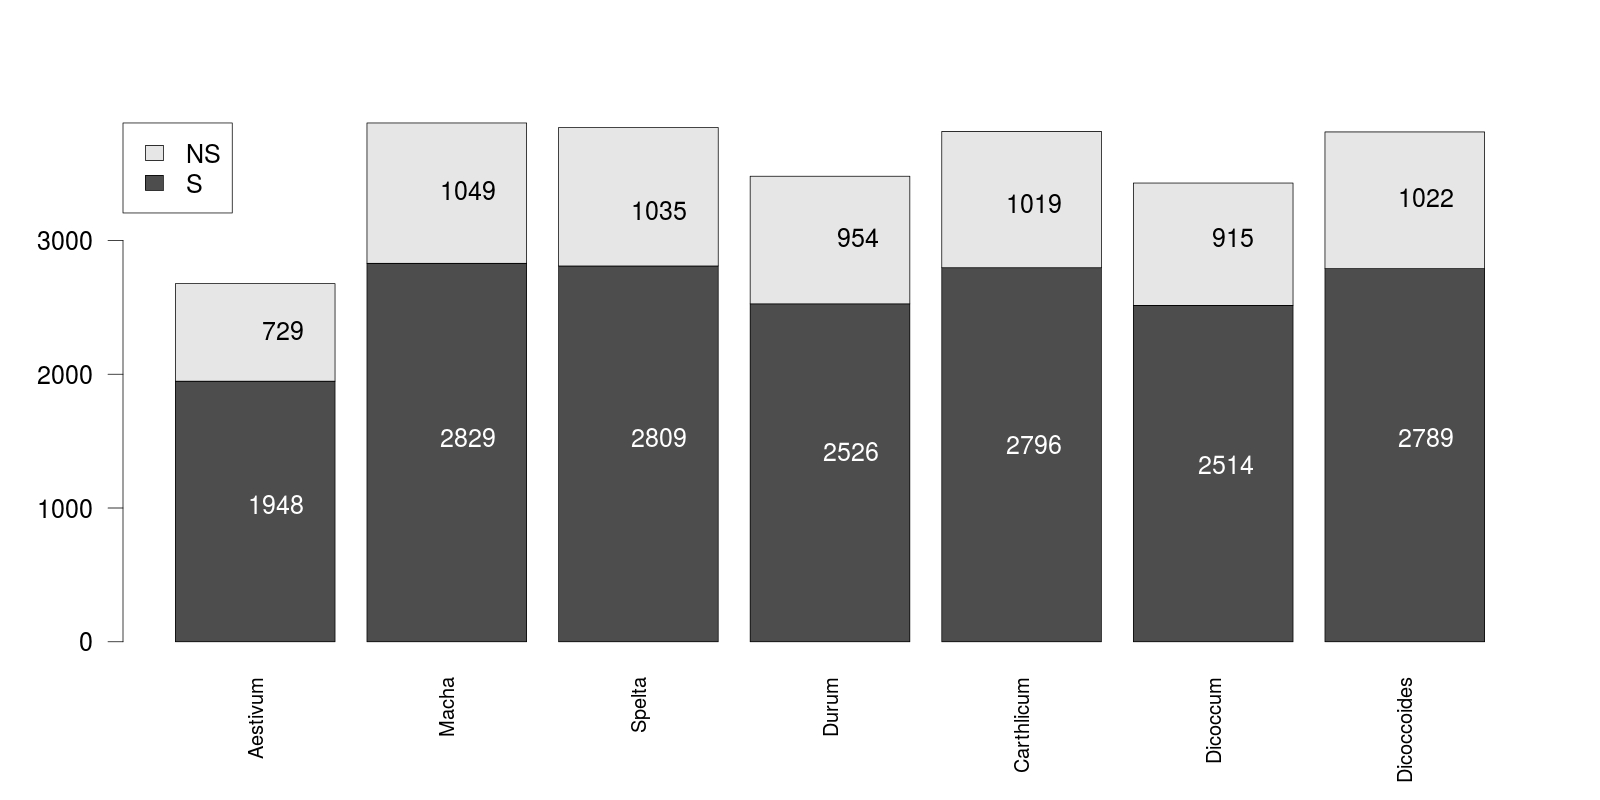
\includegraphics[scale=0.28]{Figures/Figure_22.jpg}
      \vspace{0.3cm}
      \caption{Syntenic and nonsyntenic genes in the non-variable genome of 7 \textit{Triticum}}
      \label{fig:F22}
    \footnotesize{Each bar represents the number of syntenic (dark grey) and nonsyntenic (light grey) genes in each species.}
    \end{figure}
% - - - - - - - - - - - %
    \begin{figure} 	
      \centering 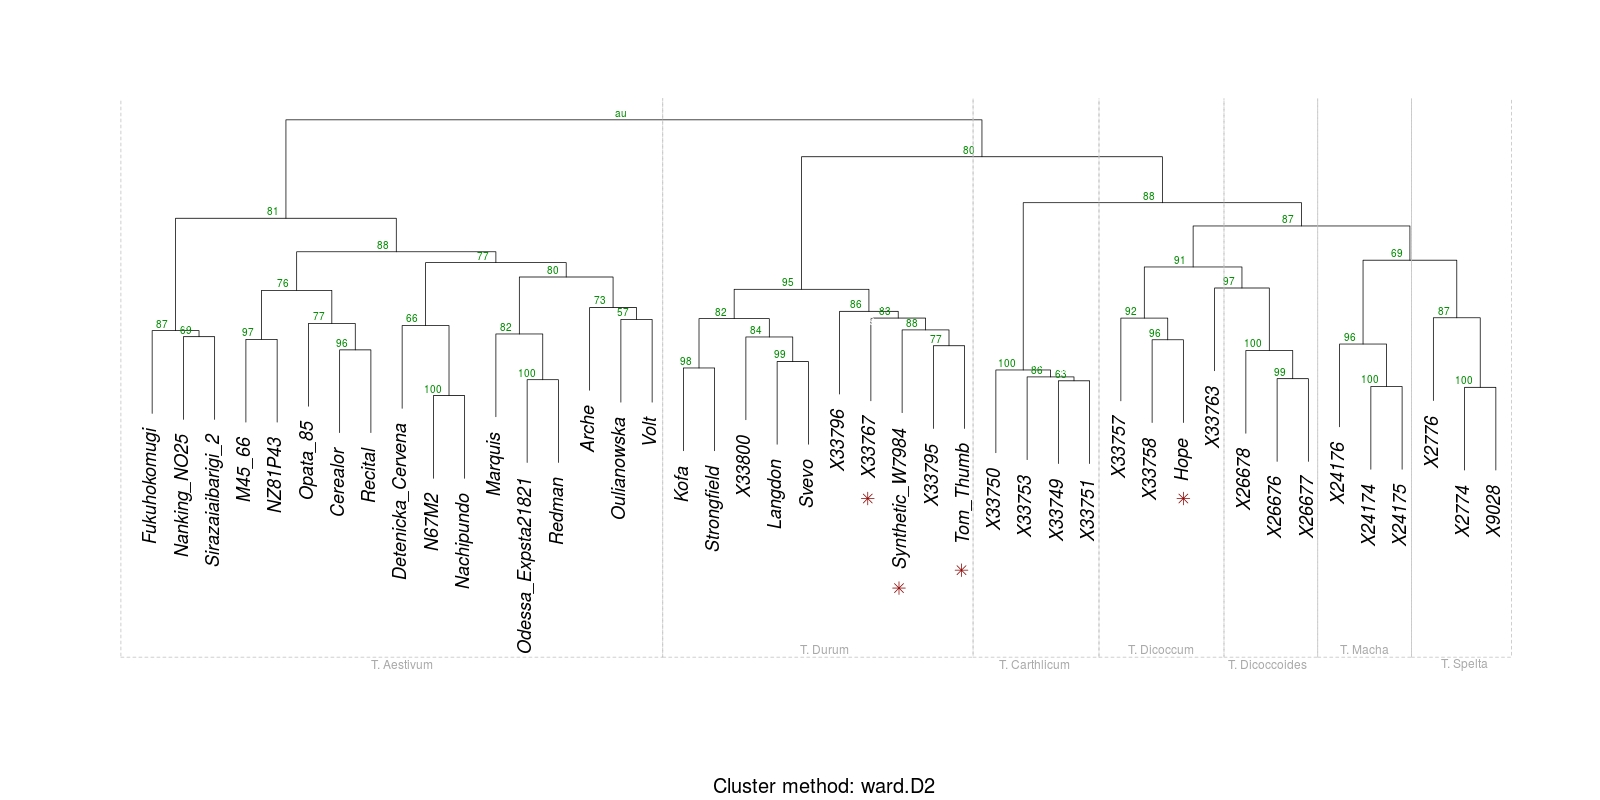
\includegraphics[scale=0.28]{Figures/Figure_23.jpg}
      \vspace{0.5cm}
      \caption{Phylogenetic tree of 44 \textit{Triticum} accessions} 
      \label{fig:F23}
    \footnotesize{The clustering by correlation with \textit{pvclust} R package uses the variation matrix to calculate distance between individuals, and gave a reliable representation. Every subfamily is grouped together except individuals marked by a red cross. Even the ploidy level is observable here, with tetraploids species grouped in the middle and flanked by hexaploid species.}
    \end{figure}
\addtocounter{page}{-1}
\newpage
\clearpage % - - - - - - - - - - - % % % FIGURE % % % - - - - - - - - - - - %

Few accessions were not placed properly according to their species. However, this can be explained when analysing their pedigree. \textit{Synthetic W7984}, \textit{Tom Thumb} and \textit{Hope} are placed on the wrong group regarding their ploidy. The \textit{T. dicoccum} specie \textit{3367} is grouped with \textit{T. durum} wheats instead of the other \textit{T. dicoccum}. 

\begin{itemize}
\item[$-$] \textit{Tom Thumb} (\textit{T. aestivum}) come from a cross with a Tibetan local variety and a \textit{T. durum}, hence their proximity.
\item[$-$] \textit{Hope} (\textit{T. aestivum}) was created by crossing \textit{Marquis} with a \textit{T. dicoccum}, that's why this accession is grouped here
\item[$-$] \textit{Synthetic W7984} (\textit{T. aestivum}) is the result of a cross between a \textit{T. durum} and \textit{Ae. tauschii}, he is thus grouped with the others \textit{durum}.
\item[$-$] \textit{33767} (\textit{T. dicoccum}) was obtained by crossing a \textit{T. dicoccum} and a \textit{T. durum}. Its 3B chromosome should have more similarities with others \textit{durum} compared to others \textit{dicoccum}.
\end{itemize}

Interestingly, beside being grouped by species, accessions were also clustered according to their geographical origin. For example, all Asian lines (\textit{Fukuhokomugi}, \textit{Nanking No25} and \textit{Sirazaiaibarigi 2}) are grouped together on the left side of the tree. Whereas the specie effect seems to have a higher impact on the clustering, this origin-based clustering suggests that SVs might be linked to specific adaptation to given environments.

    \section{Linking the studies}

        \subsection{Study of the 3B chromosome}

Last year, a work based on TEs polymorphism was done during my M1's internship. We showed that the polymorphism on the same wheat accession panel ranged from 15.8 (\textit{NZ81P43}) to 7\% (\textit{Siraizaiaibarigi 2}) of variable markers along the 3B chromosome (237,777 ISBPs in total, created with junctions between a TE and the low-copy DNA at its border).

This approach allowed to study the 85\% of the 3B chromosome composed of TEs and checked how evolution have conserved them. On the remaining 15\%, 19.81Mb (representing 2.56\% of the 3B pseudomolecule) were characterized as genes. To go deeper in the study of this chromosome, this present study was designed on genic fraction.

\newpage % - - - - - - - - - - - % % % FIGURE % % % - - - - - - - - - - - %
\thispagestyle{empty}
        \begin{figure} 	
          \centering 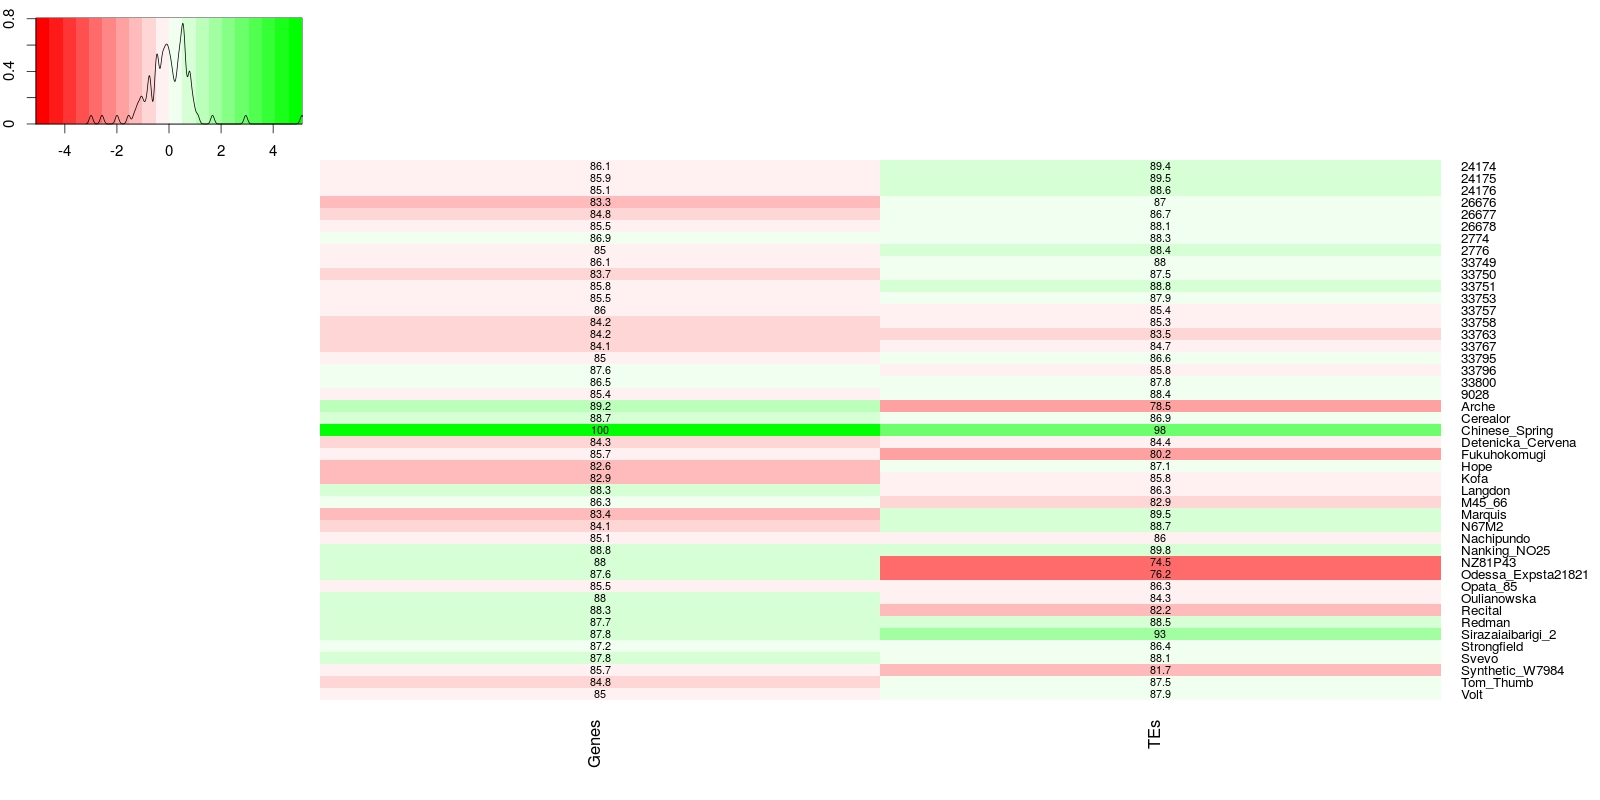
\includegraphics[scale=0.28]{Figures/Figure_24.jpg}
          \vspace{0.5cm}
          \caption{Percentage of conserved genes or TEs for each accession} 
          \label{fig:F24}
        \footnotesize{Heatmap showing the percentage of conserved marker (presence of the TE; 237,777 TEs in total) or of conserved gene (no CNV; 7,264 genes in total) between each accession and the reference \textit{Chinese Spring}. Some wheats are close to \textit{Chinese Spring} regardless the marker (\textit{Nanking No25}) and some are far (\textit{33763}). But for the majority, when TE fraction is conserved, genes are more variable, and vice-versa. The selection pressure that occurs in the DNA is different, regarding TEs or genes (Legend axis: AU).}
        \end{figure}
\addtocounter{page}{-1}
\newpage
\clearpage % - - - - - - - - - - - % % % FIGURE % % % - - - - - - - - - - - %

        \subsection{Transpositionnal and transcriptionnal}
        
By looking at the figure \ref{fig:F24}, it seems to be quite hard to establish a direct correlation between the polymorphism on repeated fraction and on genic segments on the 3B wheat chromosome. Indeed, some accession like \textit{Odessa Expsta 21821} are really divergent from \textit{Chinese Spring} regarding the TE fraction (74.5\% of conserved markers only) but quite close by looking at the genic polymorphism (88\% of conserved genes).

Some species, like \textit{T. macha} of \textit{T. spelta} seem to share more TEs with \textit{Chinese Spring}, when \textit{T. aestivum} are more conserved on genes. The tetraploids species are generally more distant from \textit{Chinese Spring}, regarding TEs or genes. The selection pressure should be thus different for these two genetic features.


% ----------------------------------------
% ----------------------------------------
% DISCUSSION
% ----------------------------------------
% ----------------------------------------
\part{Discussion / Conclusion}
\setcounter{section}{0}

Structural variations have been more and more documented over the past few years. But in plants, with large and complex genomes, only a limited number of experiments were done, and often with hybridization-based techniques. During this work, a strategy to use mapped read counts to detect CNV in genes was developed. It was so possible to detect variations with a more accurate resolution. However, several intrinsic limitations remain.

First of all, it is almost impossible to know how many copies are created or deleted by a CNV. Indeed, just increase or decrease in copy number are detectable. But it can be useful to know how many copies of a gene are deleted or duplicated, to allow a more precise correlation between genotype and phenotype. The normalization process could be improved for CNV detection in complex plant genomes for assessing exact copy number.

Then, thresholds were chosen to detect CNVs, but a more precise clustering method could be developed. As a matter of fact, instead of considering a gene as undergoing copy number variation based on an arbitrary threshold,  a statistical method such as Fisher Linear Discriminant could be used. It could create groups of individuals not only by comparison with a value, but by using the weight of each point to group them. Indeed, sometimes the normalized score of an accession is really close to the threshold, but without reaching it. In this case, it can be an error to declare there is no CNV due to the use of threshold instead of statistical method to group the points. 

\newpage % - - - - - - - - - - - % % % FIGURE % % % - - - - - - - - - - - %
\thispagestyle{empty}
~
\addtocounter{page}{-1}
\newpage
\clearpage % - - - - - - - - - - - % % % FIGURE % % % - - - - - - - - - - - %

Finally, the limited number of accessions per species analysed in this study brought some limitations. Indeed, for several analyses, a higher number of individuals could give more precise results. For example in the Venn diagrams showing the number of shared genes (Figure \ref{fig:F21}, a bias is brought by the low number of members in the \textit{T. macha} and in the \textit{T. spelta} compared to the \textit{T. aestivum}. Because of this small number of individuals in these groups, it is harder to find an accession with a variation in a gene, thus leading to a lot of shared genes between these two species. 

\vspace{0.5cm}

However, this new strategy have brought some reliable results. First, a complete methodology of CNV discovery by using mapping was developed. The mapping process indicates no bias, regardless of the position, in or out of genes and the validation with CSvCS or with the calculation of the theoretical / observed coverage. The normalization steps allow the use the number of mapped reads in a gene instead of the percentage of coverage, which can induce a covering bias by being not homogeneous along the gene. It also takes into account gene size, GC content and gene coverage in the reference accession \textit{Chinese Spring}. It is also the first work looking for CNVs in a complete gene set from a complex and highly repetitive chromosome. Indeed, Saintenac \textit{et al.} studied CNV in wheat genome, but only for two tetraploid varieties and with only 2,175 kb of coding region, versus 19.53 Mb in this work \citep{Saintenac2011}. 

Regarding the CNV results, an aCGH work made in 2013 by Muñoz-Amatriaín \textit{et al.} on barley genome revealed 14.9\% of the sequence variable in copy number and 9.5\% of the coding sequence. here we found  an average proportion of 14.49\% of the 7,264 genes variable in the 44 compared varieties. This significantly increase of variation could come from the fact that barley isn't a polyploid variety. Thus, a gene loss can be more severe for this organism, with no other subgenome available to take over, opposite to wheat which have 3 subgenomes.

Yu \textit{et al.} have defined in 2013, following a CGH work made on rice, that \textit{higher recombination rates and the presence of homologous gene clusters are probably predispositions for generation of the higher number of CNVs}, which is exactly that occurs in wheat 3B distal regions. In maize, Springer \textit{et al.} have found several short conserved clusters along chromosomes without any particular segmentation, instead of the clear partitioning of conserved and variable genes in bread wheat. However, the variations in copy number are also often found in the distal parts of the chromosomes \citep{Springer2009}. This distribution can be linked to two mechanisms:

\begin{itemize}
\item[-] Distal parts of chromosomes are more often subject to recombination. Thus, several genes could be created by DNA segments exchanges.

\newpage % - - - - - - - - - - - % % % FIGURE % % % - - - - - - - - - - - %
\thispagestyle{empty}
~
\addtocounter{page}{-1}
\newpage
\clearpage % - - - - - - - - - - - % % % FIGURE % % % - - - - - - - - - - - %

\item[-] We showed that R1/R3 regions are composed of more pseudogenes. A lot of those genic fragments could be carried by TEs, and are so more often variable in copy number. 
\end{itemize}

During the study of \textit{Arabidopsis thaliana}'s genome in 2000 by the consortium responsible for its sequencing, it was shown that genes are less present and expressed in the distal part of chromosomes, just like for the 3B ones. It so confirms the hypothesis for a wheat core genome, and more widely, a core genome of the \textit{Triticeae} localized around centromeres. 

\vspace{0.5cm}

In term of perspective, this work has to be continued on several points. First, a GO enrichment analysis has to be performed on genes designated as \textit{core} or \textit{dispensable} genome. Indeed, the core genome is expected to be enriched in genes involved in basics cellular functions, energy production, metabolic processing pathways or some other essentials cell functions. On the contrary, dispensable genes should be more involved in adaptation-related functions such as disease resistance or response to stress.

The short deletion cluster, located around 400 Mb have to be investigate. Indeed, it can come from TE activity, a tandem-duplicated gene or being an artifact.

This CNV-detection method have to be validated. Indeed, a small gene set could be chosen among the more variable and specific primers designed for their amplification by qPCR or digital PCR. Thus, we could be able to assess is a variation in copy number is really detected.

Then, the study should be redesigned as soon as more wheat 3B chromosome from others accession will be sequenced. As a matter of fact, having larger groups could give more precise results, especially for the study of shared genes among families. It could even allow to cluster more precisely each accession in the dendrogram. The panel has to be more studied too, with the aim to find the real origin of each wheat. Indeed, we just have the information about where the cross was made, and so our geographical data are not really reliable. 

However, clues were bought here concerning a core genome among the \textit{Triticeae} and is composed of 3,243 genes on the 3B chromosome, mainly located around the centromere. These genes are more often and strongly expressed. Distal parts are largely targets of CNV events, with an average of 15\% of the 3B gene set variable between the reference \textit{Chinese Spring} and an accession. 

This work is the first large scale analysis of structural variations in the wheat genome. By setting up processes to efficiently detect PAVs as well as CNVs, it paves the way for future whole-genome analyses. With the access to reference sequences of all wheat chromosomes, the availability of a growing number of resequenced accessions as well as the progresses made in sequencing technologies, such as long reads, it makes no doubt that SV analyses in wheat will soon bridge the gap with other crops species.

\end{onehalfspace}


% ----------------------------------------
% ----------------------------------------
% BIBLIOGRAPHY
% ----------------------------------------
% ----------------------------------------
\clearpage
\newpage
\pagestyle{empty}

    \part*{Bibliography}
    \renewcommand{\section}[2]{}   
    \bibliographystyle{bib_style}
    \bibliography{full_bib_2015.bib}


% ----------------------------------------
% ----------------------------------------
% APPENDIX
% ----------------------------------------
% ----------------------------------------
\newpage
\pagestyle{empty}

\begin{vcenterpage}
\part*{Appendix}
\end{vcenterpage}

\newpage
\pagestyle{empty}
\textbf{Appendix 1}: Panel of the 44 wheat varieties selected for this work.
\setlongtables
\begin{longtable}{|c|c|c|c|c|}
\hline
Name & Variety & Ploidy & Genome & Origin \\
\hline
\endfirsthead
\hline
Name & Variety & Ploidy & Genome & Origin \\
\hline
\endhead
24174 & T. macha & 6X & AABBDD & GEO \\
24175 & T. macha & 6X & AABBDD & GEO \\
24176 & T. macha & 6X & AABBDD & GEO \\
26676 & T. dicoccoides & 4X & AABB & CSK \\
26677 & T. dicoccoides & 4X & AABB & HUN \\
26678 & T. dicoccoides & 4X & AABB & CHL \\
2774 & T. spelta & 6X & AABBDD & FRA \\
2776 & T. spelta & 6X & AABBDD & FRA \\
9028 & T. spelta & 6X & AABBDD & FRA \\
33749 & T. carthlicum & 4X & AABB & GEO \\
33750 & T. carthlicum & 4X & AABB & GEO \\
33751 & T. carthlicum & 4X & AABB & GEO \\
33753 & T. carthlicum & 4X & AABB & GEO \\
33757 & T. dicoccum & 4X & AABB & IRQ \\
33758 & T. dicoccum & 4X & AABB & BGR \\
33763 & T. dicoccum & 4X & AABB & SVK \\
33767 & T. dicoccum & 4X & AABB & ISR \\
33795 & T. durum & 4X & AABB & RUS \\
33796 & T. durum & 4X & AABB & SYR \\
33800 & T. durum & 4X & AABB & TUR \\
Langdon & T. durum & 4X & AABB & USA \\
Kofa & T. durum & 4X & AABB & USA \\
Strongfield & T. durum & 4X & AABB & CAN \\
Svevo & T. durum & 4X & AABB & ITA \\
Hope & T. aestivum & 6X & AABBDD & USA \\
Marquis & T. aestivum & 6X & AABBDD & CAN \\
Arche & T. aestivum & 6X & AABBDD & FRA \\
Cerealor & T. aestivum & 6X & AABBDD & FRA \\
Chinese Spring & T. aestivum & 6X & AABBDD & CHN \\
Detenicka  Cervena & T. aestivum & 6X & AABBDD & CZE \\
Fukuhokomugi & T. aestivum & 6X & AABBDD & JPN \\
M45/66 & T. aestivum & 6X & AABBDD & ARG \\
N67M2 & T. aestivum & 6X & AABBDD & ISR \\
Nachipundo & T. aestivum & 6X & AABBDD & NPL \\
Nanking No25 & T. aestivum & 6X & AABBDD & CHN \\
NZ(81)P43 & T. aestivum & 6X & AABBDD & NZL \\
Odessa Expsta21821 & T. aestivum & 6X & AABBDD & PRT \\
Opata 85 & T. aestivum & 6X & AABBDD & MEX \\
Oulianowska & T. aestivum & 6X & AABBDD & RUS \\
Recital & T. aestivum & 6X & AABBDD & FRA \\
Redman & T. aestivum & 6X & AABBDD & CAN \\
Sirazaiabarigi 2 & T. aestivum & 6X & AABBDD & JPN \\
Tom Thumb & T. aestivum & 6X & AABBDD & USA \\
Volt & T. aestivum & 6X & AABBDD & HUN \\
W7984 (Synthetic) & T. aestivum & 6X & AABBDD & MEX \\
\hline
\end{longtable}

\newpage
\pagestyle{empty}
\textbf{Appendix 2}: Workflow of the mapping process. Reads coming from the 44 3B chromosomes were mapped onto the reference sequence from \textit{Chinese Spring}. The genic fractions were extracted from the mapping data and the number of reads for each accession in each gene was calculated. After a normalization process, a matrix containing coverages for every gene for the 44 varieties was created.

\vspace{3cm}

\centering 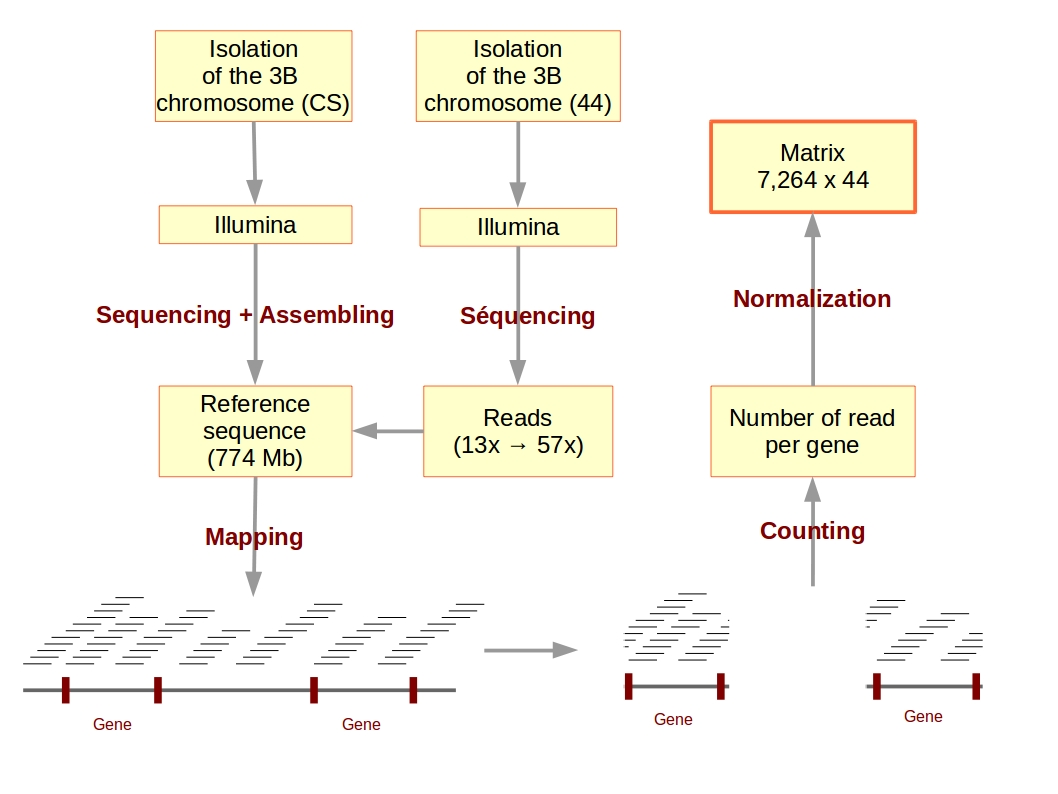
\includegraphics[scale=0.4]{appendix/Appendix_3.jpg}

\newpage
\pagestyle{empty}
    \textbf{Appendix 3}: Representation of every lost gene for each accession along the 3B chromosome. Each bar represent a lost gene and the colours are function of the specie (red \textit{macha}, blue \textit{dicoccoides}, orange \textit{spelta}, purple \textit{carthlicum}, green \textit{dicoccum}, brown \textit{durum} and light blue \textit{aestivum}. A short cluster around 400 Mb is visible and each distal region is subject to more gene loss than the C region.
    
\vspace{1cm}

\centering 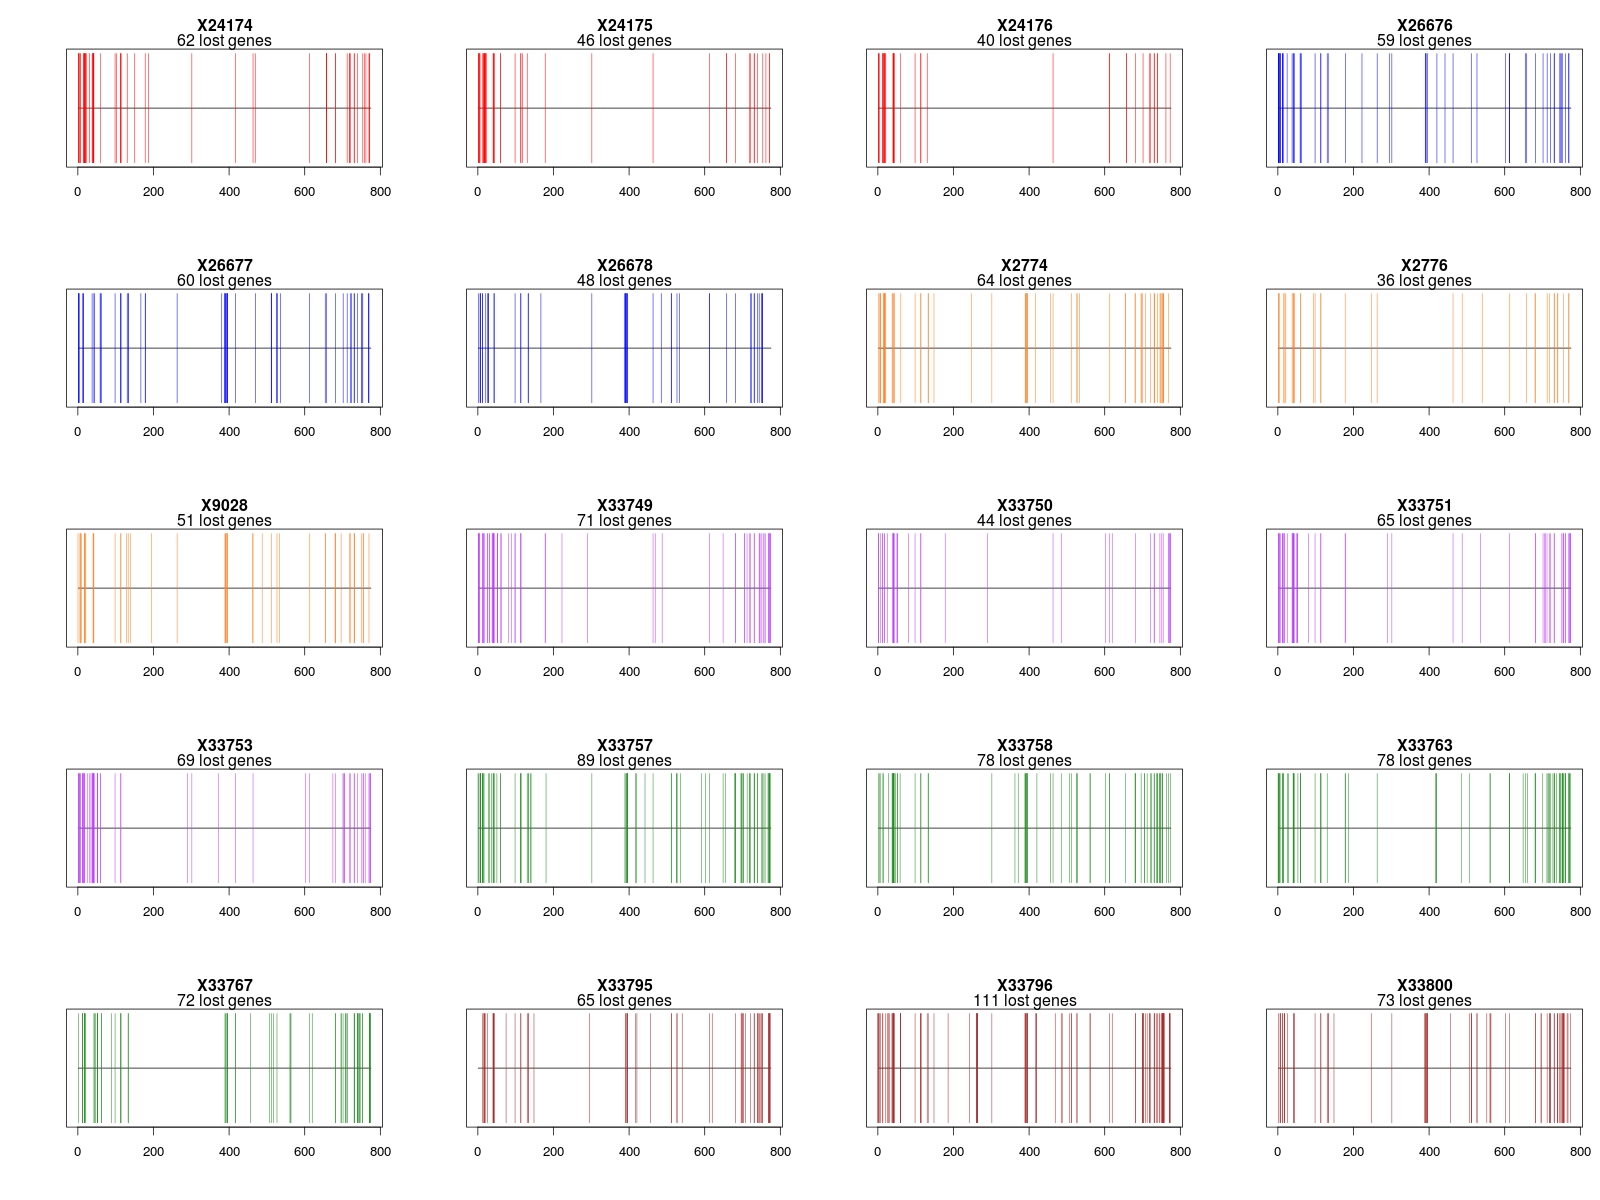
\includegraphics[scale=0.28]{appendix/Appendix_4_1.jpg}
\newpage
\pagestyle{empty}
\centering 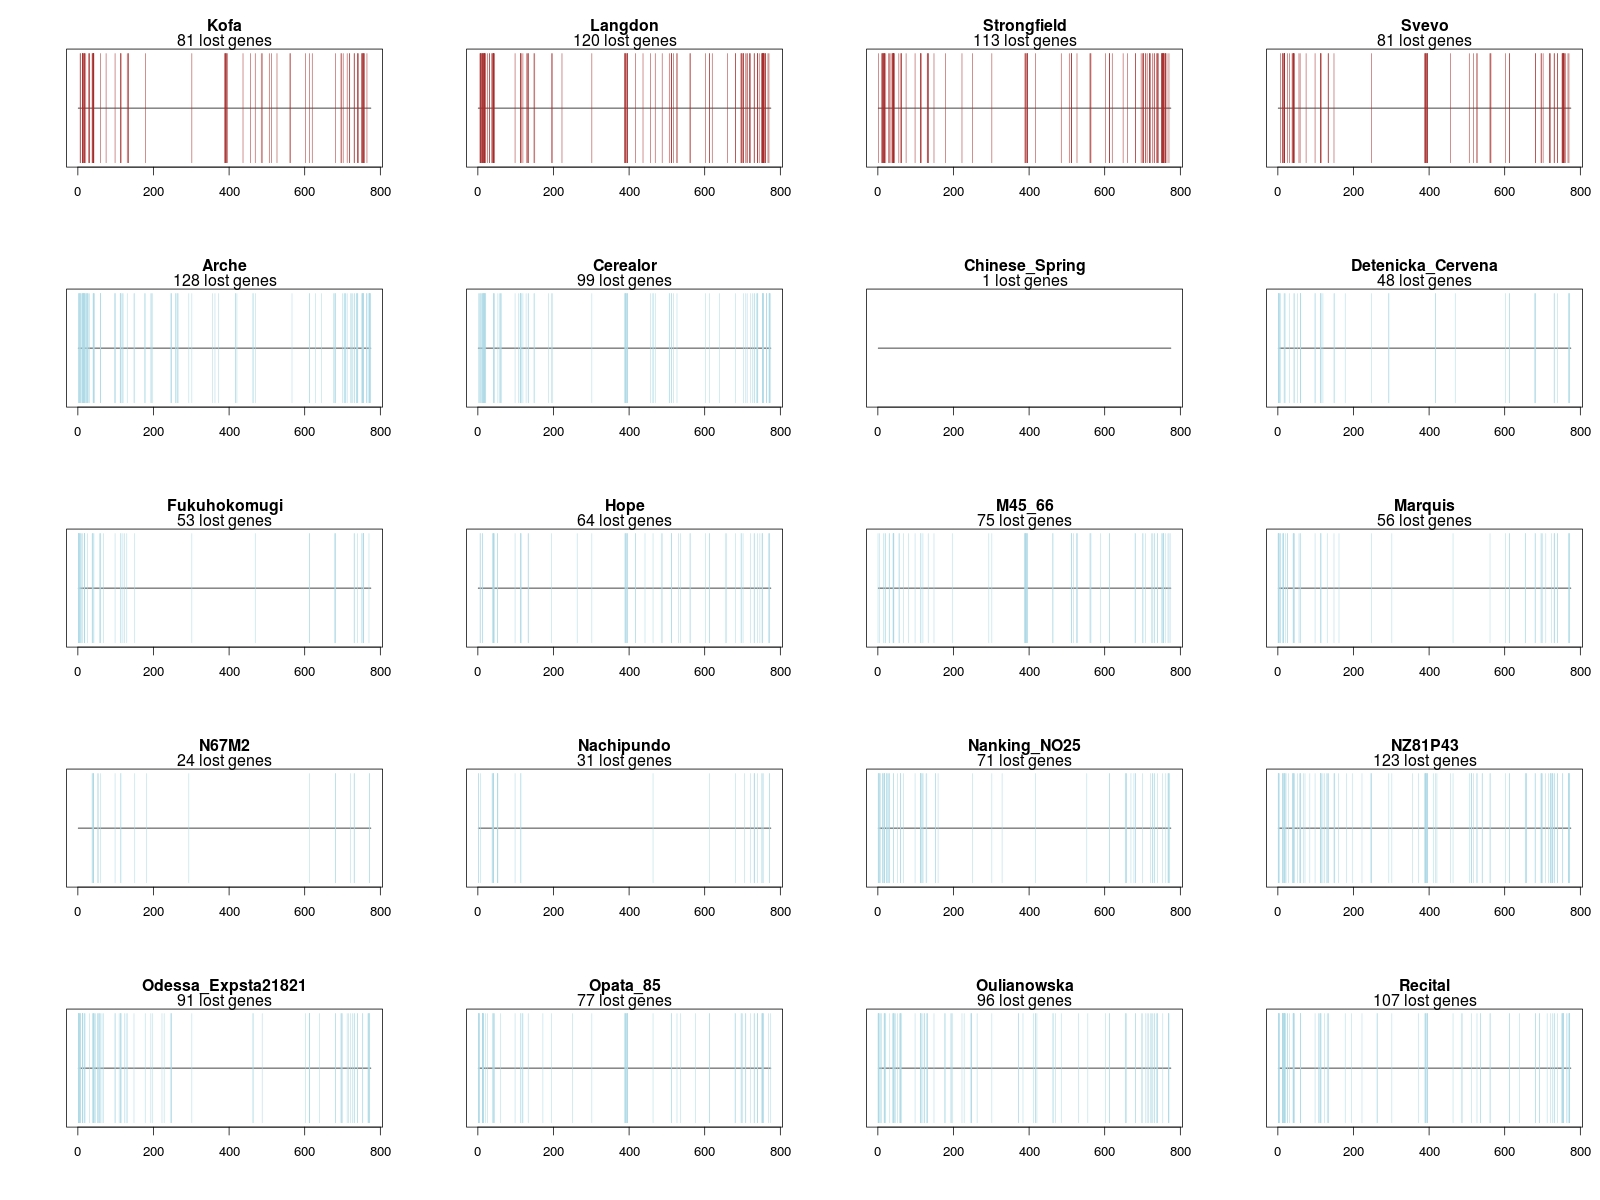
\includegraphics[scale=0.28]{appendix/Appendix_4_2.jpg}
\centering 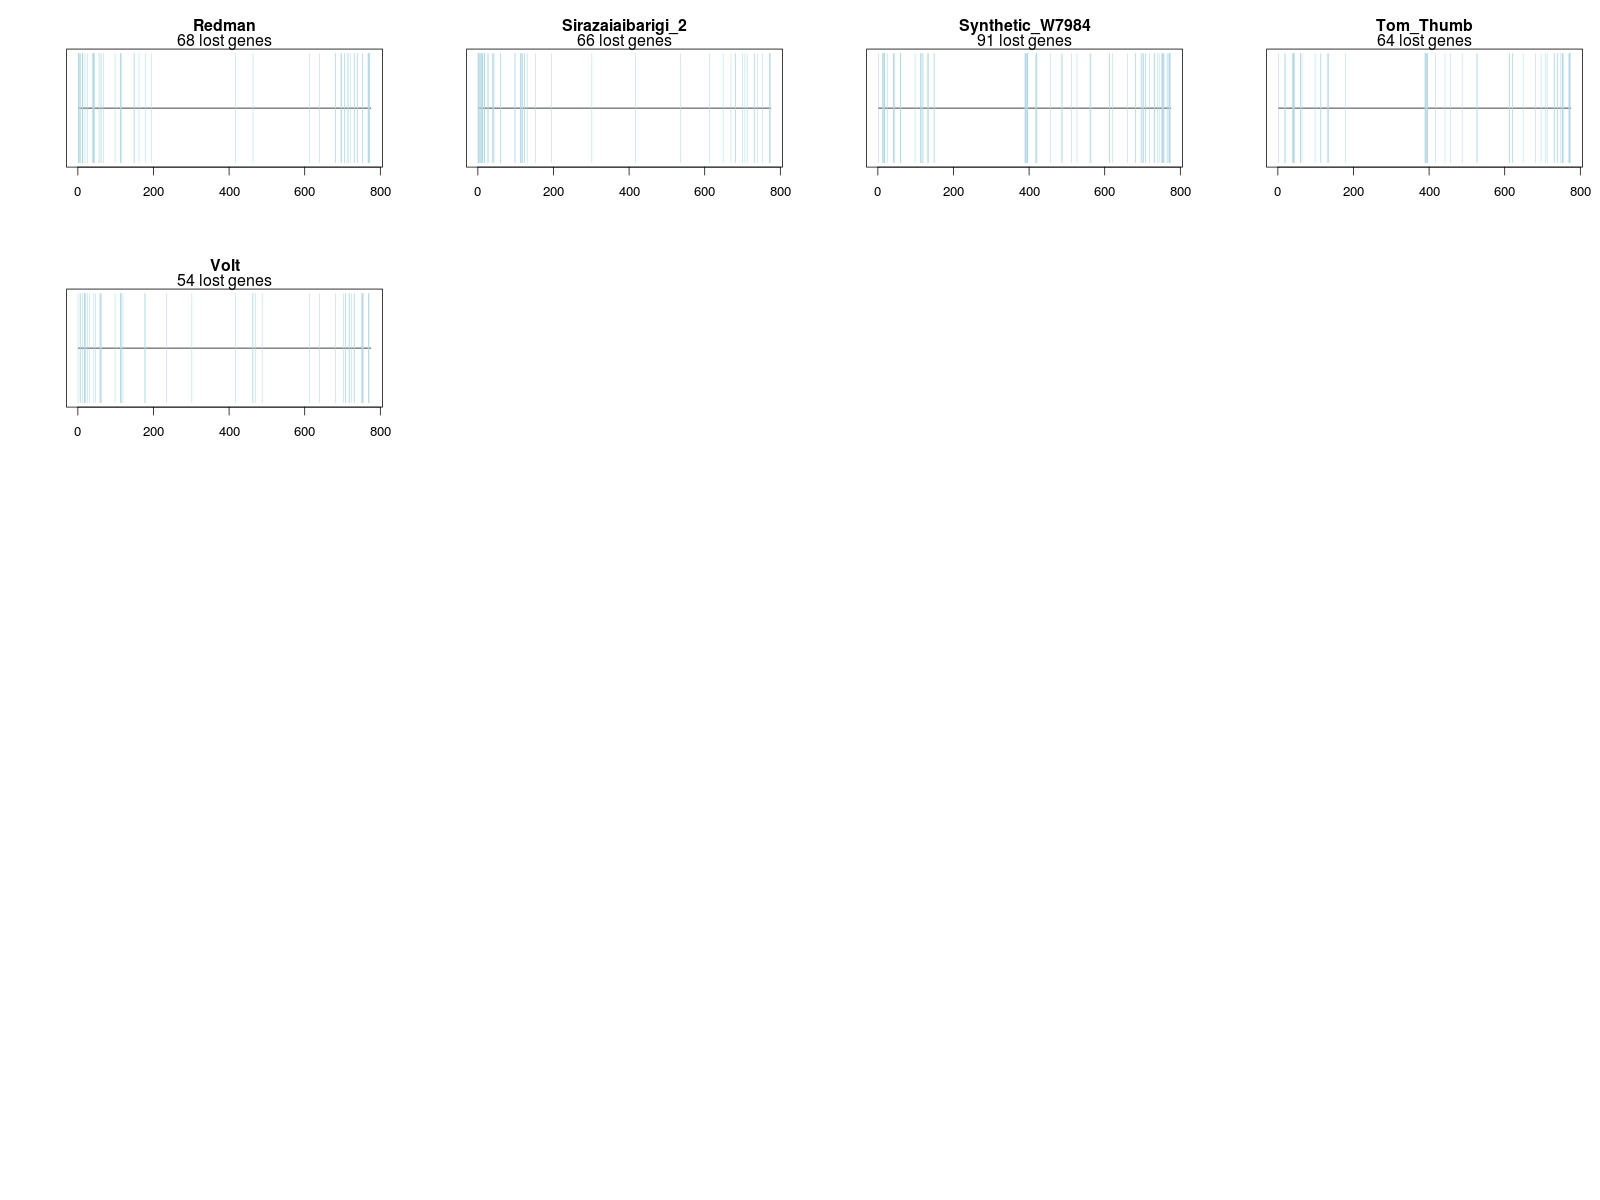
\includegraphics[scale=0.28]{appendix/Appendix_4_3.jpg}

\newpage
\pagestyle{empty}
    \textbf{Appendix 4}: Representation of the decreases in copy number (deletions, red curves) and increases in copy number (duplications, green curves) for every accession. Genes are largely more variable in the distal part of the chromosome arms.
    
\vspace{1cm}

\centering 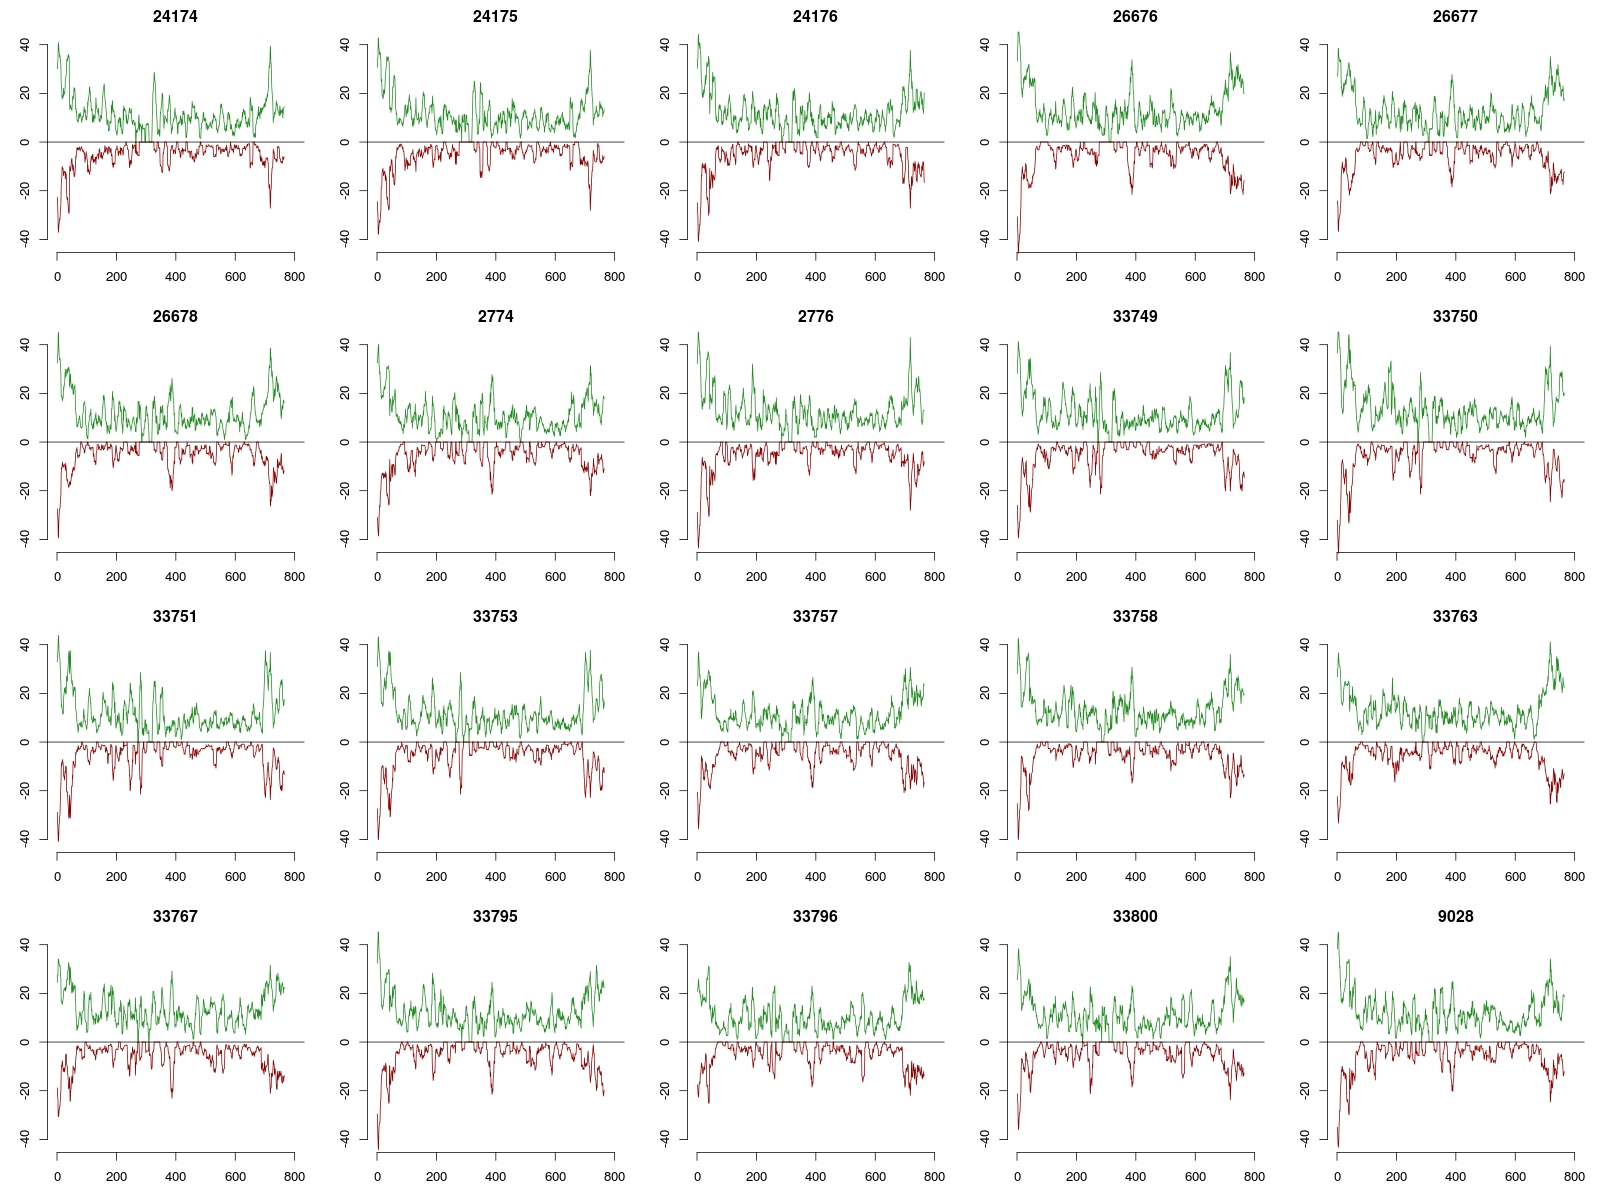
\includegraphics[scale=0.28]{appendix/Appendix_5_1.jpg}
\newpage
\pagestyle{empty}
\centering 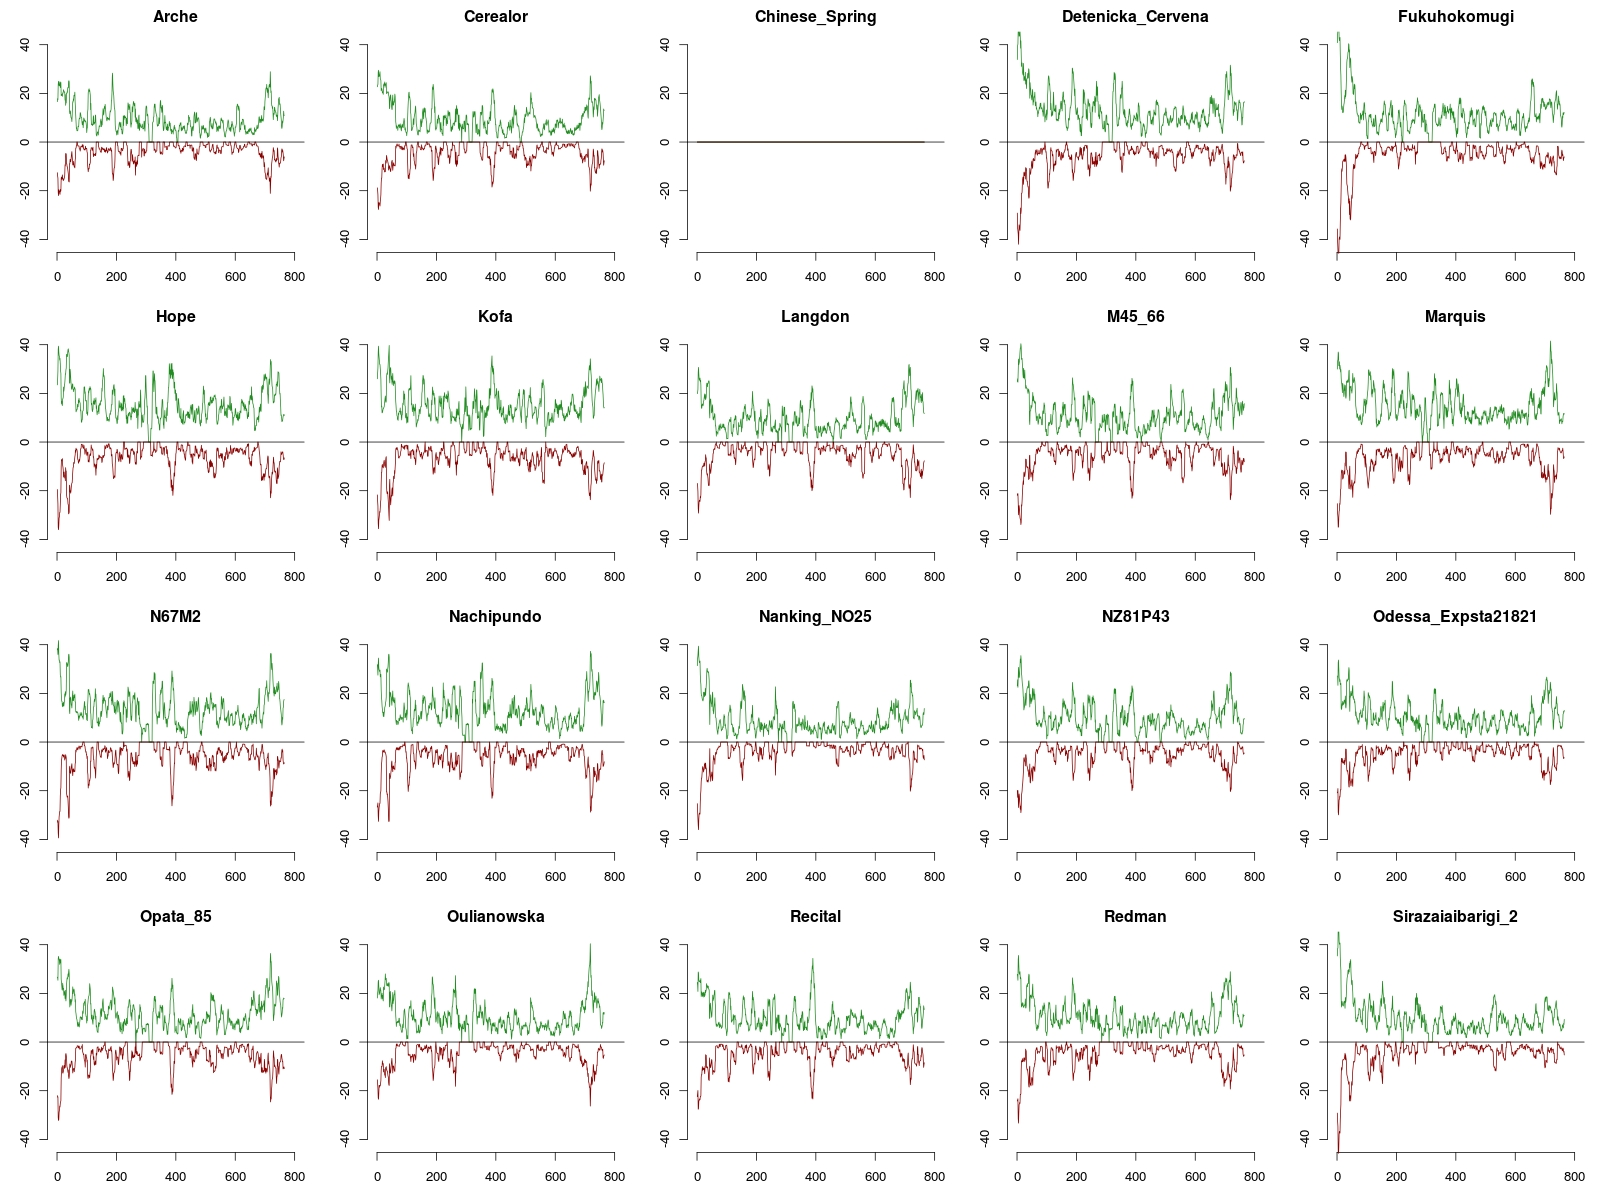
\includegraphics[scale=0.28]{appendix/Appendix_5_2.jpg}
\centering 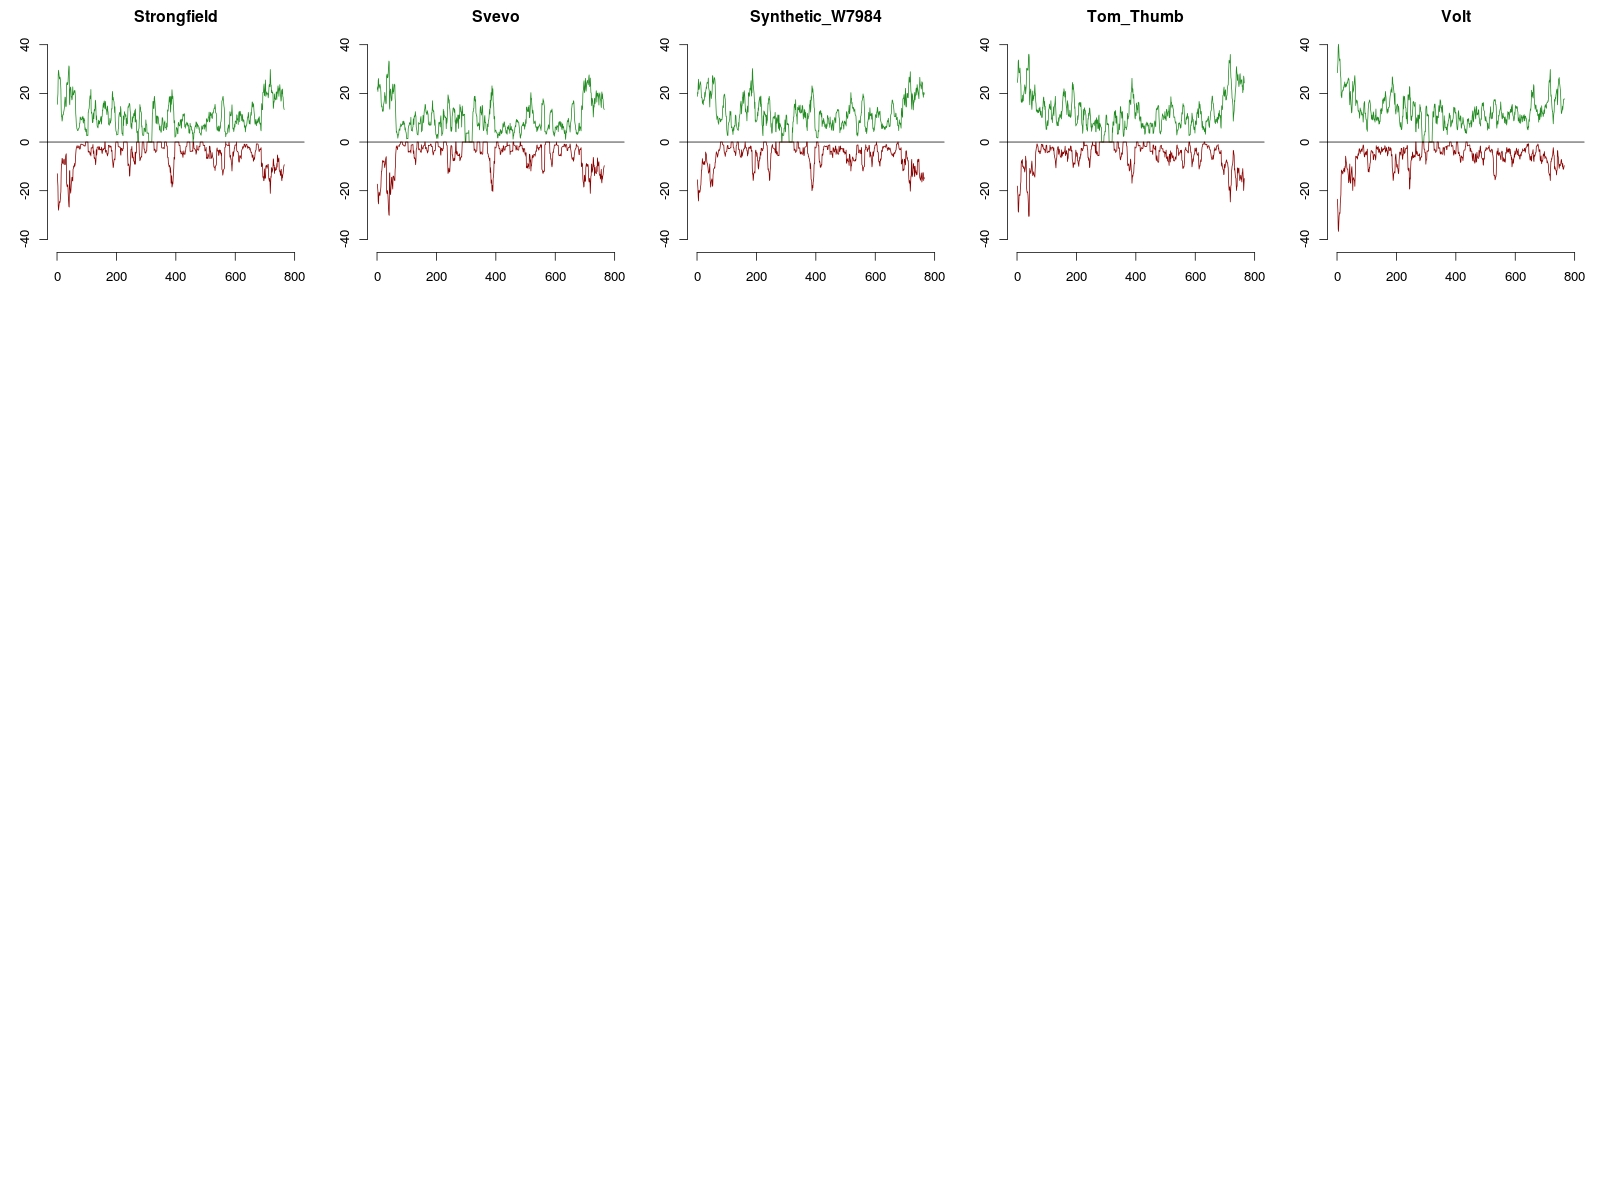
\includegraphics[scale=0.28]{appendix/Appendix_5_3.jpg}

\end{document}